\documentclass[titlepage,10pt]{book}
%\usepackage[pdfpagelabels,draft,implicit=false]{hyperref}
\usepackage{ifthen}

\providecommand\documentlanguage{SK}



\usepackage[utf8]{inputenc}
\usepackage[usenames,dvipsnames]{xcolor}
\usepackage{colortbl}
\usepackage{a4wide}
\usepackage{amssymb,amsmath,amsthm}
\usepackage{xspace}
\usepackage{tikz}
\usepackage{tikz-3dplot}
\usepackage{eurosym}
\usepackage[usenames]{xcolor}
\usepackage{calc}
%\usepackage{framed}
\usepackage{mdframed}
\usepackage{array}
\usepackage{graphicx}
\usepackage{hvfloat}
\usepackage{multirow}
\usepackage{algorithmicx}
\usepackage[ruled]{algorithm}
\usepackage{algpseudocode}
\usepackage{mathrsfs}
\usepackage{refcount}
\usepackage{fncychap}
%\usepackage[english]{babel}
%\usepackage{blindtext}
\usepackage{pgffor}
\usepackage{fontawesome}

\usepackage{etoolbox}
\BeforeBeginEnvironment{framed}{\vskip 1ex\begin{minipage}{\linewidth}}
\AfterEndEnvironment{framed}{\end{minipage}\vskip 1ex}

\usetikzlibrary{intersections}
\usetikzlibrary{arrows,matrix,positioning,decorations.pathreplacing}

\ifthenelse{ \equal{\documentlanguage}{SK} }{
  \usepackage[slovak]{babel}
  %\usepackage[babel=true,kerning=true]{microtype}
  \usetikzlibrary{babel}
}{}

\newcommand{\ie}{i.e.,\xspace}

\makeatletter
\renewcommand{\DOCH}{}
\renewcommand{\DOTI}[1]{%
  \vspace*{-2.1cm}
  \hrule
  \vskip 3mm
  {\huge\bfseries\thechapter}\hfill{\LARGE\bfseries #1}
  \vskip 3mm
  \hrule
  \par\nobreak
\vskip 40\p@}
\makeatother


\usepackage{chngcntr}
\counterwithout{equation}{chapter}

\newmdenv[linewidth=1pt]{framed}
\newmdenv[backgroundcolor=shadecolor,hidealllines=true ]{shaded}

\newcommand{\todo}[1]{ }



\renewcommand{\mod}{\ensuremath{\mathrm{mod\ }}}
\renewcommand{\neg}[1]{\overline{#1}}
\newcommand{\algA}{{\tt A}\xspace}

\newcommand{\probname}[1]{\hbox{\sc #1}\xspace}
\newcommand{\sat}{\probname{Sat}}
\newcommand{\maxsat}{\probname{Max-Sat}}
\newcommand{\maxcut}{\probname{Max-Cut}}
\newcommand{\minvcover}{\probname{Min-Vertex-Cover}}
\newcommand{\maxflow}{\probname{Max-Flow}}
\newcommand{\maxWBmatching}{\probname{Max-Weighted-Bipartite-Matching}}
\newcommand{\maxis}{\probname{Max-Independent-Set}}
\newcommand{\minmulticut}{\probname{Min-Multi-Cut}}
\newcommand{\mincut}{\probname{Min-Cut}}
\newcommand{\minfactor}{\probname{Min-1-Factor}}
\newcommand{\binpacking}{\probname{Bin-Packing}}
\newcommand{\mingap}{\probname{Generalized-Assignment}}
\newcommand{\minsforest}{\probname{Min-Steiner-Forest}}
\newcommand{\member}{\probname{2D-Membership}}
\newcommand{\multiwaycut}{\probname{Min-Multiway-Cut}}
\newcommand{\kcut}{\probname{Min-$k$-Cut}}
\newcommand{\knapsack}{\probname{Max-Knapsack}}
\newcommand{\Qknapsack}{\probname{Max-Q-Knapsack}}
\newcommand{\minpartition}{\probname{Min-Partition}}

\newcommand{\pair}[2]{\ensuremath{\left\langle #1,#2\right\rangle}}
\newcommand{\bpair}[2]{\ensuremath{\left\langle\bm{#1},\bm{#2}\right\rangle}}

\newcommand{\dom}{\ensuremath{{\cal D}}\xspace}

\newcommand{\NP}{\ensuremath{NP}\xspace}
\newcommand{\APX}{\ensuremath{APX}\xspace}
\newcommand{\PTAS}{\ensuremath{PTAS}\xspace}
\newcommand{\FPTAS}{\ensuremath{FPTAS}\xspace}
\renewcommand{\P}{\ensuremath{P}\xspace}

\newcommand{\bm}[1]{\mbox{\boldmath{$\rm#1$}}}
\newcommand{\tr}{\ensuremath{^{\sf T}}}
\newcommand{\opt}{\ensuremath{OPT}\xspace}
\newcommand{\T}{\ensuremath{{\cal T}}}
\newcommand{\R}{{\mathbb R}}
\newcommand{\Z}{{\mathbb Z}}
\renewcommand{\S}{\ensuremath{\mathscr{S}}}


\newcommand{\alg}[1]{\ensuremath{\mathtt{#1}}\xspace}


\newcommand{\ev}[1]{\ensuremath{{\mathrm E}\left[#1\right]}}
\newcommand{\pr}[1]{\ensuremath{\mathrm{Pr}\left[#1\right]}}
\newcommand{\Deg}{\ensuremath{\mathrm{deg}}}

\newcommand{\cvect}[1]{\ensuremath{\left(\begin{array}{c}#1\end{array}\right)}}

\newcommand{\common}{}
\newcommand{\commonii}{}
\newcommand{\axes}{}
\newdimen\picx
\newdimen\picy

\newcounter{dummy} \numberwithin{dummy}{chapter}

%%%%%%%%%%%%%%%%%%%%%%%%%%%%%%%%%%%%%%%%%%%%%%%%%%%%%
% slovak stuff
\ifthenelse{ \equal{\documentlanguage}{SK} }{
\newtheorem{veta}[dummy]{Veta}
\newtheorem{veta-star}[dummy]{$\star$ Veta}
\newtheorem{lema}[dummy]{Lema}
\newtheorem{dosl}[dummy]{Dôsledok}

\theoremstyle{definition}
\newtheorem{dfn}[dummy]{Definícia}
\newtheorem{clm}[dummy]{Tvrdenie}
\newtheorem*{ozn}{Označenie}
\newtheorem*{prob}{Cvičenie}

\newenvironment{dokaz}{\begin{proof}[{\bfseries Dôkaz:}]}{\end{proof}}
\newenvironment{dokazpar}[1]{\begin{proof}[{\bfseries Dôkaz #1:}]}{\end{proof}}
\newcommand{\bulpar}{\vskip 4pt\noindent{\bf $\bullet$ }}

}{% english stuff
%  \newcommand{\ie}{i.e.,\xspace}

\newtheorem{veta}[dummy]{Theorem}
\newtheorem{veta-star}[dummy]{$\star$ Theorem}
\newtheorem{lema}[dummy]{Lemma}
\newtheorem{dosl}[dummy]{Corollary}

\theoremstyle{definition}
\newtheorem{dfn}[dummy]{Definition}
\newtheorem{clm}[dummy]{Claim}
\newtheorem*{ozn}{Notation}
\newtheorem*{prob}{Exercise}

\newenvironment{dokaz}{\begin{proof}[{\bfseries Proof:}]}{\end{proof}}
\newenvironment{dokazpar}[1]{\begin{proof}[{\bfseries Proof #1:}]}{\end{proof}}
\newcommand{\bulpar}{\vskip 4pt\noindent{\bf $\bullet$ }}

}
%%%%%%%%%%%%%%%%%%%%%%%%%%%%%%%%%%%%%%%%%%%%%%%%%%%%%


\newenvironment{myfig}[2]{\vskip 4pt\noindent\begin{center}\includegraphics[width=#1]{#2.pdf}\\[1ex]
  \begin{minipage}[t]{0.9\textwidth}\bgroup\small}{%
  \egroup\end{minipage}\end{center}\vskip 4pt\noindent}

\newenvironment{myfiglabel}[3]{\vskip 4pt\noindent
    \phantom{aa}\hfill
    \begin{minipage}[c]{#1-4ex}
      \vskip 0pt
      \includegraphics[width=\textwidth]{#2.pdf}
    \end{minipage}
    \hfill
    \begin{minipage}[c]{4ex}
      \vskip 0pt
      \begin{equation}\label{#3}~\end{equation}
    \end{minipage}
    \vskip 1ex
    \begin{center}
  \begin{minipage}[t]{0.9\textwidth}\bgroup\small}{%
  \egroup\end{minipage}\end{center}\vskip 4pt\noindent}

\newcommand{\mycaption}[1]{\vskip 1ex\noindent{\small #1}\vskip 4pt\noindent}



\newcommand{\optional}{{\LARGE$\star$ }}

\newcommand{\IGNORE}[1]{}
\newcommand{\TODO}{\vskip 1ex\noindent{\em plánované}}


\newcommand{\tmp}{}

\bibliographystyle{abbrv}
\setlength{\parindent}{0pt}

\begin{document}
\nocite{A99,WS11,GLS88,MG07,SST06,KM72,V04,Ch83,Bland77,LBILS01,H99,ST04,BBC04,EF03,L94}
\pagestyle{empty}
\phantom{A}
\vfill
\centerline{\rule{0.8\textwidth}{0.5ex}}
\hrule
\vskip 3mm
\centerline{\Large\bfseries\sc Optimization and Approximation}
\vskip 3mm
\hrule
\centerline{\rule{0.8\textwidth}{0.5ex}}
\vfill
Rasťo Královič\hfill (preliminary $\alpha$ version)  \hfill \today
\newpage
\phantom{A}
\newpage
\section*{About}

This text was created as part of the project ``Príprava štúdia matematiky a informatiky na FMFI UK 
v anglickom jazyku'', ITMS: 26140230008, funded by the EU.
\vfill
\noindent
In the text, the following graphics were used: \\
\begin{itemize}
  \item unit sprites from the project ''Battle for Wesnoth'' {\tt http://www.wesnoth.org}
  \item binder graphics from the project digstud {\tt https://github.com/bitfragment/digstud.git}
  \item images of printers from manufacturers' web presentations
\end{itemize}


\newpage
\tableofcontents
\newpage
\setcounter{page}{1}
\pagestyle{plain}

\chapter{Linear programming}
\typeout{EEEEEEEEEEEEE \thepage EEEEEEEEEEEEEEEEE}

% % % % % % % % % % % % % % % % % % % % % % % % % % % % % % % % % % % % % % % %
\section{A gentle introduction}

Let us start with an example that is, in some of its many forms, a must
in any text about linear programming. Let us have a student  
going to pull an all-nighter in preparation for some exam. In order to 
stay awake he needs to get at least 
$270$~mg of caffeine, and at least $120$~g of sugar. At the same time,
a dose of more than $180$~mg of aspartame may be hazardous to his health. 
He can choose between two drinks: brown stuff for \hbox{\EUR{$1$}/dl}, and
green stuff for \hbox{\EUR{$1,50$}/dl.}
1 dl of brown stuff contains  $30$~mg of caffeine, $40$~g of sugar, and
$40$~mg of aspartame, while the same amount of green stuff contains
$90$~mg of caffeine, $30$~g of sugar, and $30$~mg of aspartame. 
How much of which stuff should the student buy in order to satisfy all his needs
at the smallest possible cost?
If he buys $x$~dl of brown stuff, and $y$~dl of green stuff, the problem
(called a {\em linear program}) can be formulated as follows:


\begin{equation}
  \label{eq:LP:1}
\begin{array}{rccccll}
                          & \multicolumn{3}{c}{\text{dl of stuff}} \\ 
                          & \text{brown} & & \text{green}\\
  {\rm minimize}     & x   & + & 1.5 y & =: & f(x,y) &  \text{\em price}\\
  {\rm subject\ to} & \color{blue}{30 x } & \color{blue}{+} & \color{blue}{90 y} & \color{blue}{\ge} & \color{blue}{270} & \text{\color{blue}{\em caffeine}}\\ 
                           & \color{red}{40 x}   & \color{red}{+}  & \color{red}{30 y}  & \color{red}{\ge} & \color{red}{120} & \text{\color{red}{\em sugar}} \\
                           & \color{magenta}{40 x} & \color{magenta}{+} & \color{magenta}{30 y} & \color{magenta}{\le} & \color{magenta}{180} & \text{\color{magenta}{\em aspartame}}\\
                          &      &   & x,y  &\ge& 0
\end{array}
\end{equation}
%
It is easy to see that, e.g., $4$~dl of green stuff satisfy all the requirements
at the cost of \EUR{6}, while providing even more caffeine than necessary, and
less aspartame than allowed. On the other hand, if the student would be buying
only brown stuff, in order to satisfy his needs for caffeine he would have
to buy 9~dl of it, which would overdose him with aspartame (and it would be
too costly anyway).
When looking for the optimal optimal solution the following geometric interpretation
comes handy: to each solution with $x$~dl of brown stuff, and $y$~dl of green stuff
assign a point $(x,y)$ in the plane. Each of the constraints then defines a half-plane
where a feasible solution can be located. Hence, all feasible solutions lie in the
quadrilateral on the left:


% draws a halfplane
% optional: paameters to draw
% fist point, second point, orientation (+/-), length1, length2
\newcommand{\halfplane}[6][ ]{%
  \coordinate (O) at (#2);
  \coordinate (XX) at (#3);
  \coordinate (YY) at ($ (O) !1! 90:(XX) $);
  \coordinate (X) at ($ (XX) - (O) $);
  \coordinate (Y) at ($ (YY) - (O) $);
  \coordinate (E) at ($ (XX)!#6! ($(XX)+(X)$) $);
  \begin{scope}[#1]
      \draw 
          ($ (O)!-#5!(XX) $) -- (E);
     
      \foreach \i in {0,0.1,...,1}  
          \draw
          let
              \p1 = ($ ($ (E) !1.5cm! (O) $) + ($ (0,0) !\i cm! (X) $) $)
         in
              (\p1) -- ($ (\p1) ! 8pt ! #4 330:($ (\p1)+($ (0,0)#4(Y) $) $) $);
  \end{scope}
}


\renewcommand{\common}{%
  %axis
  \draw (-2,0) -- coordinate (x axis mid) (11,0);
  \draw (0,-2) -- coordinate (y axis mid) (0,8);
  %ticks
  \foreach \x in {-2,...,10}
      \draw (\x,1pt) -- (\x,-3pt);
  \foreach \x in {2,4,...,10}
      \draw (\x,-3pt) node[anchor=north] {\x};
  \foreach \y in {1,...,7}
      \draw (1pt,\y) -- (-3pt,\y) 
          node[anchor=east] {\y}; 
      \draw (0,0) node[anchor=north east]{$0$};
  %labels      
      \node[below=0.8cm] at (x axis mid) {brown stuff};
  \node[rotate=90] at (-2,4) {green stuff};
  
  \filldraw[fill=black!50, line width=0.8pt, fill opacity=0.5 ]
    (0,6) -- (0,4) -- (1,2.66) -- (3,2) -- cycle;
}


\begin{center}
\begin{tikzpicture}[scale=0.5]

  \halfplane[color=red]{0,4}{3,0}{+}{1cm}{1cm}
  \halfplane[color=blue]{9,0}{0,3}{-}{1cm}{1cm}
  \halfplane[color=magenta]{0,6}{4.5,0}{-}{1cm}{1cm}

  \common
\end{tikzpicture}
\hfill
\begin{tikzpicture}[scale=0.5]
  \begin{scope}
    \clip (-1,-0.4) -- (11,-0.4) -- (11,8) -- (-1,8) -- cycle;
    \coordinate (v) at (3,-2);
    \draw[dashed,color=black!80]  
        \foreach \p in {(1,2.66),(0,4),(0,6),(0,7)}
            {($ (\p ! 20cm ! ($ (\p - (v) $) $)  -- ($ (\p ! 20cm ! ($ (\p + (v) $) $)};
    \coordinate (q) at ($ (0,7) !4cm! ($ (0,7) + (v) $) $);
    \draw[thick,->]
        (5,6) node[anchor=south west] {$f(x,y)=10.5$}  -- (q) ;
  \end{scope}
  
      
  \common
  \filldraw[very thin,red,dotted]
        (1,2.66) circle (2pt) -- (0,2.66)
        (1, 2.66) -- (1,0);
\end{tikzpicture}
\end{center}
%
At the same time we know that $f(x,y)=x+1.5y$ is a linear function, so points
with the same value of $f$ form a straight line (see the right figure). Now it should
be clear that in order to find the optimal solution it is sufficient to
to check the four corners of the quadrilateral and conclude that the best thing
to do is to buy $1$~dl of brown stuff, and $2\frac{2}{3}$~dl of green stuff for \EUR{5}.


\noindent
\begin{minipage}[t]{\textwidth-6cm}
\vspace{0pt}
The previous ideas lead directly to a simple algorithm for solving the problem with
two variables, and a number of inequality constraints: for each constraint consider the
corresponding half-plane, construct the (convex) polygon that is the intersection 
of all these halfplanes, and choose the optimal solution from among all its vertices.
With three variables, the constraints are of the form $a_1x+a_2y+a_3z\ge b$, and they 
define half-spaces in 3D, whose intersection is a polyhedron. Points with the
same value of the function $f(x,y,z)=c_1x+c_2y+c_3z$ form a plane, and so it is sufficient to
check all the vertices of the polyhedron to find the optimal solution.\\
\end{minipage}
\begin{minipage}[t]{6cm}
  \vspace{0pt}
  % origin, side (vector), second side
\newcommand{\kvad}[3]{%
    (#1) -- ($ (#1) + (#2) $) -- ($ (#1) + (#2) + (#3) $) -- ($ (#1) + (#3) $) -- cycle
}

% new_point_name x y z  (RotatedOriginShift should be set)
\newcommand{\rottomain}[4]{
    \tdplottransformrotmain{#2}{#3}{#4}
    \coordinate (#1) at ($ (\tdplotresx,\tdplotresy,\tdplotresz) + (RotatedOriginShift) $);
}

% intersection of two lines: name and four endpoints
\newcommand{\intersect}[5]{
    \path [name path=intersect_p1] (#2) -- (#3);
    \path [name path=intersect_p2] (#4) -- (#5);
    \path [name intersections={of=intersect_p1 and intersect_p2, by={#1}} ];
}

\renewcommand{\axes}{%
    \draw[thick,->] 
      (0,0,0) -- (1.3,0,0) node[anchor=north east]{$x$}
      (0,0,0) -- (0,1.3,0) node[anchor=north west]{$y$}
      (0,0,0) -- (0,0,1.3) node[anchor=south]{$z$};
    \draw[thick,->,tdplot_rotated_coords,color=blue] 
      (0,0,0) -- (1,0,0) node[anchor=north east]{$x$}
      (0,0,0) -- (0,1,0) node[anchor=north west]{$y$}
      (0,0,0) -- (0,0,1) node[anchor=south]{$z$};
}

\begin{center}
  \tdplotsetmaincoords{70}{60}
  \begin{tikzpicture}[scale=2,tdplot_main_coords]

    \tdplotsetrotatedcoords{45}{55}{5}    
    \coordinate (RotatedOriginShift) at (1,1,1);
    \tdplotsetrotatedcoordsorigin{(RotatedOriginShift)}
    %\axes       

    \fill[fill=black!30,fill opacity=0.3]
        \kvad{0,0,0}{1,0,0}{0,1,0}
        \kvad{0,0,0}{0,1,0}{0,0,1}
        \kvad{1,1,1}{-1,0,0}{0,0,-1}
        \kvad{1,1,1}{0,-1,0}{0,0,-1};
    \fill[fill=black!90, fill opacity=0.3]
        \kvad{0,0,0}{1,0,0}{0,0,1};
    \fill[fill=black!50, fill opacity=0.3]
        \kvad{0,0,1}{1,0,0}{0,1,0};
        

  
    % blue kvad  
    \rottomain{p1}{-0.7}{-1}{0} % origin
    \rottomain{p2}{0.7}{-1}{0}  % o + x
    \rottomain{p3}{-0.7}{1}{0}  % o + y

    \intersect{i1}{p1}{p2}{1,0,1}{1,1,1}
    \intersect{i2}{p1}{p3}{0,0,1}{0,1,1}
    \intersect{i3}{p1}{p2}{1,1,0}{1,1,1}

    \draw
        (1,0,1) -- (i1)
        (0,0,1) -- (i2)
        (1,1,0) -- (i3)
        \kvad{0,0,0}{1,0,0}{0,0,1}
        (1,0,0) -- (1,1,0);

    \draw[dashed]    
        (i1) -- (1,1,1)
        (0,1,0) -- (1,1,0)
        (0,1,0) -- (0,0,0)
        (0,1,0) -- (0,1,1)
        (i2) -- (0,1,1)
        (i3) -- (1,1,1)
        (0,1,1) -- (1,1,1);

    \begin{scope}[tdplot_rotated_coords]
       \filldraw[color=blue,very thin,fill=blue!20,fill opacity=0.5]
          \kvad{-0.7,-1,0}{1.4,0,0}{0,2,0};
        %\draw[color=blue,very thick,->]  
        %  (0,0,0) -- (0,0,1);
        \fill[color=blue]
          (0,0,0) circle (1pt);
    \end{scope}


  \end{tikzpicture}
\end{center}

\end{minipage}


\noindent 
With increasing the number of variables, however, many problems arise, and it
soon becomes clear that a straightforward generalization is a road to hell. 
Let us have a different look at the geometry of the linear program. First, 
let us rewrite program (\ref{eq:LP:1}) to an equivalent form as follows:
multiply the function $f(x,y)$ by -1, and from minimization problem we get a maximization.
Then also premultiply by -1 the first and second constraint to get all the constraints
(except those $x,y\ge0$) in the ``$\le$'' form. Finally, since in each constraint the 
left hand side is smaller than the right hand side, we can add a new non-negative variable 
to represent the difference between the right hand side and the left hand side. These
transformations yield the following linear program which is obviously equivalent to the original one:

\begin{equation}
\label{eq:LP:2}
\begin{array}{rrrrrrcl}
  {\rm maximmize}     & -x   & -  1.5y &         &         &       & =: & f(x,y,s_1,s_2,s_3) \\
   {\rm subject\ to}& -30x & -  90y  & +   s_1 &         &       & =  & -270\\
                          & -40x & -  30y  &         & +   s_2 &       & =  & -120\\
                          &  40x & +  30y  &         &         &+  s_3 & =  & 180\\      
                          &      &         &     \multicolumn{3}{r}{x,y,s_1,s_2,s_3}  &\ge& 0
\end{array}
\end{equation}
%
If we denote
\begin{align*}
 \bm{c}&=\cvect{-1\\-1.5\\0\\0\\0}
&A&=\left(\begin{array}{ccccc}-30&-90&1&0&0\\-40&-30&0&1&0\\30&40&0&0&1\end{array}\right)
&\bm{b}&=\cvect{-270\\-120\\200}
\end{align*}
then the program (\ref{eq:LP:2}) can be written concisely
$$\max_{\bm{x}\in\R^5}\left\{ \bm{c}\tr\bm{x} \mid A\bm{x}=\bm{b},\; \bm{x}\ge0
\right\}.$$ 
The transformation increased the dimension of the problem from 2 to 5 (and we lost the possibility
of a graphical solution), but the gain is a nicer set of feasible solutions: feasible solutions
are non-negative solutions of a system of linear equations. In our case the matrix $A$ has rank 3
(the rows are linearly independent) and the solutions of the system
$A\bm{x}=\bm{b}$ 
form a two-dimensional subspace
$\bm{o}+c_1\bm{\alpha}+c_2\bm{\beta}$ where
\begin{align*}
\bm{o}&=\cvect{0\\0\\-270\\-120\\180}
      &\bm{\alpha}&=\cvect{1\\0\\30\\40\\-40}
      &\bm{\beta}&=\cvect{0\\1\\90\\30\\-30}.
\end{align*}
In other words, the feasible solutions of program (\ref{eq:LP:1}) 
form a 2-dimensional polygon (quadrilateral) in a 2-dimensional subspace (a plane),
while the feasible solutions of program (\ref{eq:LP:2}) form a 2-dimensional 
polygon \dom in a 5-dimensional space, where \dom is the intersection of a (2-dimensional)
plane with the positive orthant\footnote{in the same spirit as ''quadrant'' in 2D, and ''octant''
in 3D, we use the term ''orthant'' in a general $n$-dimensional space}. 
To illustrate this, consider the following simple programs (we show only the constraints, the 
utility function does not matter in this case):


\renewcommand{\commonii}{%
  %axis
  \draw (-0.5,0) -- coordinate (x axis mid) (1.5,0);
  \draw (0,-0.2) -- coordinate (y axis mid) (0,1.5);
  %ticks
  \foreach \x in {-0.2,-0.1,...,1.4}
      \draw (\x,1pt) -- (\x,-3pt);
  \draw (1,-3pt) node[anchor=north] {1};

  \foreach \y in {0.2,0.3,...,1.4}
      \draw (1pt,\y) -- (-3pt,\y);
  \draw (-1pt,1) node[anchor=east] {1}; 
  
  \draw (0,-3pt) node[anchor=north east]{$0$};
}


\renewcommand{\axes}{
    \draw
      (0,0,0) -- (1.5,0,0) node[anchor=north east]{$x$}
      (0,0,0) -- (0,1.5,0) node[anchor=north west]{$y$}
      (0,0,0) -- (0,0,1.5) node[anchor=south]{$s$};
}


\setlength{\picx}{(0.5\textwidth - 3cm)/2}
\setlength{\picy}{\picx}
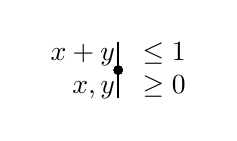
\begin{tikzpicture}[x=\picx,y=\picy]
  \fill[fill=blue!50, opacity=0.8]
    (0,0) -- (1,0) -- (0,1) -- cycle;
  \commonii
  \draw[thick, shorten >= -10pt, shorten <= -10pt] (0,1) -- (1,0);
  \draw (0.7,1) node {$\begin{array}{rl}x+y&\le 1\\ x,y&\ge0\end{array}$};
  \foreach \p in {(0,0),(1,0),(0,1)}
    \filldraw \p circle (1.5pt); 
\end{tikzpicture}
\hfill
\tdplotsetmaincoords{70}{120}
\begin{tikzpicture}[scale=2.3,tdplot_main_coords]
  \axes
  \coordinate (u) at ($ (0,0,0)!2.5cm!(-1,1,0) $);
  \coordinate (v) at ($ (0,0,0)!2cm!(-1,-1,2) $);
  \coordinate (p) at ($ (1,0,0)!7mm! ($ (1,0,0)-($(u)+(v)$) $) $);
  
  \filldraw[fill=blue!30, opacity=0.3]
      (p) -- ($ (p) + (u) $) -- ($ (p) + (u) + (v) $) -- ($ (p) + (v) $) -- cycle;
  \draw[thin]
      (p) -- ($ (p) + (u) $) -- ($ (p) + (u) + (v) $) -- ($ (p) + (v) $) -- cycle;

  \filldraw[thick,fill=blue!50, opacity=0.8]
      (1,0,0) -- (0,1,0) -- (0,0,1) -- cycle;
  \foreach \p in {(1,0,0),(0,1,0),(0,0,1)}
    \filldraw \p circle (.8pt); 
 
   \draw[tdplot_screen_coords] (0.7,1) node {$\begin{array}{rl}x+y+s&= 1\\ x,y,s&\ge0\end{array}$};

\end{tikzpicture}

\noindent 
On the left there is a program with two variables and a 2-dimensional solution space. 
After the transformation into three dimensions the solution space remained 2-dimensional,
and it is the intersection of a plane with the positive octant. In the next example
the original problem has a 1-dimensional solution space. After the transformation into three
dimensions it is still 1-dimensional, and it is an intersection of a line with the positive octant.

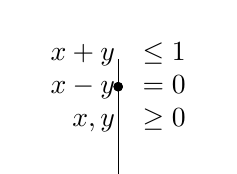
\begin{tikzpicture}[x=\picx,y=\picy]
  \fill[fill=blue!30, opacity=0.3]
    (0,0) -- (1,0) -- (0,1) -- cycle;
  \draw[shorten >= -2cm, shorten <= -3pt] (0,0) -- (.5,.5);
  \draw[very thick]
    (0,0) -- (0.5,0.5);
  \commonii
  \draw[shorten >= -10pt, shorten <= -10pt] (0,1) -- (1,0);

  \draw (0.6,1.5) node {$\begin{array}{rl}x+y&\le 1\\ x-y&=0\\x,y&\ge0\end{array}$};
  \foreach \p in {(0,0),(.5,.5)}
    \filldraw \p circle (1.5pt); 
\end{tikzpicture}
\hfill
\tdplotsetmaincoords{70}{120}
\begin{tikzpicture}[scale=2.3,tdplot_main_coords]
  \axes
  \coordinate (u) at ($ (0,0,0)!2.5cm!(-1,1,0) $);
  \coordinate (v) at ($ (0,0,0)!2cm!(-1,-1,2) $);
  \coordinate (p) at ($ (1,0,0)!7mm! ($ (1,0,0)-($(u)+(v)$) $) $);
  
  \filldraw[fill=blue!30, opacity=0.3]
      (p) -- ($ (p) + (u) $) -- ($ (p) + (u) + (v) $) -- ($ (p) + (v) $) -- cycle;
  \draw[thin]
      (p) -- ($ (p) + (u) $) -- ($ (p) + (u) + (v) $) -- ($ (p) + (v) $) -- cycle;

  \coordinate (u) at ($ (0,0,0)!1cm!(1,1,0) $);
  \coordinate (v) at ($ (0,0,0)!1.8cm!(0,0,1) $);
  \coordinate (p) at ($ (0,0,0)!3mm! ($ (0,0,0)-($(u)+(v)$) $) $);
  
  \filldraw[fill=green!30, opacity=0.3]
      (p) -- ($ (p) + (u) $) -- ($ (p) + (u) + (v) $) -- ($ (p) + (v) $) -- cycle;
  \draw[thin]
      (p) -- ($ (p) + (u) $) -- ($ (p) + (u) + (v) $) -- ($ (p) + (v) $) -- cycle;
  

  \filldraw[color=blue!60, fill=blue!50, opacity=0.5]
      (1,0,0) -- (0,1,0) -- (0,0,1) -- cycle;
  \filldraw[color=green!60, fill=green!50, opacity=0.5]
      (0,0,0) -- (0,0,1) -- (.5,.5,0) -- cycle;


  \foreach \p in {(0,0,1),(.5,.5,0)}
    \filldraw \p circle (.8pt); 
 
  \draw[tdplot_screen_coords] (0.7,1.05) node {$\begin{array}{rl}x+y+s&=1\\ x-y&=0\\x,y,s&\ge0\end{array}$};
  \draw[very thin, dashed] 
      (0,0,0) -- (1.5,1.5,0)
      (0,0,0) -- (0,0,1)
      (1,0,0) -- (0,1,0) -- (0,0,1) -- cycle;
  \draw[very thick]
    (0,0,1) -- (0.5,0.5,0);

\end{tikzpicture}

\noindent 
The advantage of this form of the linear program is that it is easier to 
identify the vertices of the polygon of feasible solutions: they lie in some face of 
the form $x_i=0$.

Before continuing in our musings it is good to note that we may, without loss of generality,
suppose that the rows of the matrix $A$ are linearly independent:
if there is a row that is a linear combination of some other rows, then either there is
no feasible solution at all, or by leaving out that row the set of feasible solutions 
remains the same. We can summarize our ideas, and define a {\em normal form} of a linear program
as follows:

\vskip 1em
\noindent
\begin{framed}
  \begin{dfn}
  \label{df:LP:eqnormalform}
  A linear program is in the {\bf normal form}, if it is written as
\begin{equation}
  \max_{\bm{x}\in\R^n}\left\{ \bm{c}\tr\bm{x} \mid A\bm{x}=\bm{b},\;\bm{x}\ge\bm{0}\right\},
\end{equation}
where $A\in\R^{m\times n}$ has rank $m$. The set of feasible solutions $\dom=\left\{\bm{x}\in\R^n \mid  A\bm{x}=\bm{b},\;\bm{x}\ge\bm{0}\right\}$.
\end{dfn}
\end{framed}

\begin{itemize}
\item {\bf The goal is maximization.} 
  If the original goal was to minimize a linear function
$f(\bm{x})$, 
the new goal is to maximize the (linear) function
$-f(\bm{x})$.
\item {\bf All variables are non-negative.} 
Each variable $x$ that is not bound by a constraint $x\ge0$
will be replaced by two variables $p_x, q_x\ge0$, and each occurrence
of $x$ in will be replaced by $p_x0q_x$.
\item {\bf Each constraint, except for those $x\ge0$ has the form of equality}.
  A constraint of the form $\sum_ia_ix_i\ge b$ is first multiplied by $-1$ on
  both sides, turning it into $\sum_i-a_ix_i\le-b$. After all constraints
  have the inequalities facing the same direction, a new variable $s$ ({\em slack})
  is introduced for each constraint $\sum_ia_ix_i\le b$; this variable represents
  the extent to which the equality is violated, \ie 
 $s\ge 0$, and $s+\sum_ia_ix_i=b$.  
\item {\bf The matrix \bm{A} has full rank, \ie has \bm{m} linearly independent rows.}
\end{itemize} 

\noindent 
Now let us have a program in the normal form. In a way similar to the opening example,
we want to find the set of vertices (corners) of the polyhedron \dom of the feasible solutions,
so it is sufficient to check those vertices in order to find the optimal solution.
Since \dom is formed by the intersection of the solution space of the system $A\bm{x}=\bm{b}$
with the positive orthant, its corners have some (at least one)  coordinates 
$x_{i_1},\ldots,x_{i_k}$ zero (the hyperplane $x_i=0$ is on the border of the orthant). 
Moreover, the corners are ''pointy'' (unlike the points in some face $x_i=0$ where, say,
a whole line segment lies). The ''pointyness'' of a vertex can be formulated the following
way: if the constraints $A\bm{x}=\bm{b}$
are augmented by the set of equations  $x_{i_1}=0,\ldots,x_{i_k}=0$,
the resulting system has a unique solution (\ie a ''corner'' lies in the 
intersection of some of the boundary faces of the orthant, and no other point lies
in the same intersection). Since $A$ has full rank $m$, in order to have a unique
solution of the system, we need $k=n-m$. 

\noindent Now let us get back to program (\ref{eq:LP:2}).  The matrix $A$ has rank 3,
so the vertices of \dom are obtained by augmenting the system  $A\bm{x}=\bm{b}$ 
by two constraints $x_i=0$, and $x_j=0$. In this way, 10 different equation systems can 
be obtained, with the following solutions:


\vskip 1ex
{
\renewcommand{\arraystretch}{1.5}
\renewcommand{\tmp}[3]{\multicolumn{1}{#1>{\columncolor[gray]{0.9} $}#2<{$}#3}}

\noindent
\begin{minipage}[c]{6cm}
  \vskip 0pt
\begin{tabular}{|>{$}r<{$}|>{$}c<{$}>{$}c<{$}>{$}c<{$}>{$}c<{$}>{$}c<{$}|c}\cline{1-6}
    \text{constraints}   & x   & y        & s_1 & s_2 & s_3  \\\cline{1-6}
  \rule{0mm}{3ex}                x=y=0  & 0     & 0          & -270  & -120  & 180  \\
                             x=s_1=0  & 0     & 3          & 0     & -30   & 90    \\
 \tmp{|}{r}{|}{x=s_2=0} & \tmp{}{c}{}{0}     & \tmp{}{c}{}{4}  & \tmp{}{c}{}{90}    &  \tmp{}{c}{}{0}    & \tmp{}{c}{|}{60} & A \\
 \tmp{|}{r}{|}{x=s_3=0} & \tmp{}{c}{}{0}     & \tmp{}{c}{}{6}  & \tmp{}{c}{}{270}   &  \tmp{}{c}{}{60}   & \tmp{}{c}{|}{0} & B\\
                y=s_1=0 & 9     & 0          & 0     &  240  &  -180 \\
                y=s_2=0 & 3     & 0          & -180  &  0    &  60\\
                y=s_3=0 & 4.5 & 0          & -135  &  60   &  0\\
 \tmp{|}{r}{|}{\bm{s_1=s_2=0}} & \tmp{}{c}{}{\bm{1}}     &\tmp{}{c}{}{\bm{\frac{8}{3}}} & \tmp{}{c}{}{\bm{0}}     &  \tmp{}{c}{}{\bm{0}}    &  \tmp{}{c}{|}{\bm{60}}& C\\
 \tmp{|}{r}{|}{s_1=s_3=0}      & \tmp{}{c}{}{3}     &\tmp{}{c}{}{2}           & \tmp{}{c}{}{0}     &  \tmp{}{c}{}{60}   &  \tmp{}{c}{|}{0} & D\\
                                  s_2=s_3=0&\multicolumn{5}{c|}{no solution}\\\cline{1-6}
  \end{tabular}
\end{minipage}
\hfill
\begin{minipage}[c]{5.6cm}
  \vskip 0pt
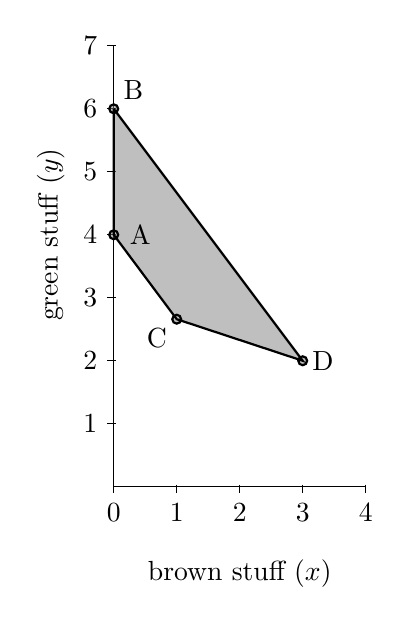
\begin{tikzpicture}[scale=0.8]
  %axis
  \draw (0,0) -- coordinate (x axis mid) (4,0);
  \draw (0,0) -- coordinate (y axis mid) (0,7);
  %ticks
  \foreach \x in {0,...,4}
      \draw (\x,1pt) -- (\x,-3pt);
  \foreach \x in {0,...,4}
      \draw (\x,-3pt) node[anchor=north] {\x};
  \foreach \y in {1,...,7}
      \draw (1pt,\y) -- (-3pt,\y) 
          node[anchor=east] {\y}; 
  %labels      
  \node[below=0.8cm] at (x axis mid) {brown stuff ($x$)};
  \node[rotate=90] at (-1,4) {green stuff ($y$)};
  
  \filldraw[fill=black!50, line width=0.8pt, fill opacity=0.5 ]
    (0,6) -- (0,4) -- (1,2.66) -- (3,2) -- (0,6)
    (0,6) circle (2pt)
    (0,4) circle (2pt)
    (1,2.66) circle (2pt)
    (3,2) circle (2pt);

    \draw (0,6) node[anchor=south west]{B};  
    \draw (.1,4) node[anchor=west]{A};  
    \draw (3,2) node[anchor=west]{D};  
    \draw (1,2.66) node[anchor=north east]{C};  
\end{tikzpicture}
\end{minipage}

}

\vskip 2ex
\noindent 
The solutions of the system $A\bm{x}=\bm{b}$ form a (2-dimensional) plane
in a 5-dimensional space. The variables  $x,y$ represent the amounts
of brown and green stuff, respectively, the variables $s_1,s_2,s_3$
give the slack of the corresponding constraint.
So, for example, the fourth row of the table with constraints $x=s_3=0$
tells us that if the student doesn't buy any brown stuff, and at the same
time he wants to reach the exact allowed intake of aspartame, he has to buy 
6~dl of the green stuff, while he gets more caffeine and sugar than needs.
The last row shows that the constraints can not be added arbitrarily,
but care must be taken not to introduce any linearly dependent rows (in our case
the red and purple lines from the first figure are parallel, so there is no
point in their intersection). In the language of linear programs the rows of
this table are called {\em basic solutions} and those among them that are also
feasible (the highlighted rows) are {\em feasible basic solutions}, and correspond
to the vertices of \dom; in our case the feasible solutions of the program (\ref{eq:LP:2})
form a (2-dimensional) quadrilateral in a 5-dimensional space.

\noindent
It is worth noting that the feasible basic solutions of the program
(\ref{eq:LP:2}), \ie the vertices of the quadrilateral of feasible solutions
in the 5-dimensional space correspond in a straightforward way to the 
vertices of the quadrilateral of the feasible solutions of the program
(\ref{eq:LP:1}): each vertex of the quadrilateral on the right is 
an intersection of two lines corresponding to a constraint  $x_i=0$ 
(and the respective basic solution is feasible). On the other hand, 
every feasible basic solution is the intersection of two such lines.

\vskip 1ex
\noindent
Noting that the introduction of a constraint $x=0$ actually deletes a column
corresponding to the variable $x$ from the respective equation system, 
we arrive to the following definition:

\begin{ozn}
Let  $A\in\R^{m\times n}$ be a matrix with  $m$ rows and $n$ columns. Given a set
$B\subseteq\{1,2,\ldots,n\}$, the symbol $A_B$ denotes the submatrix of $A$
consisting of columns indexed by the set $B$. The same notation
$\bm{x}_B$ 
will be used for vectors.
\end{ozn}

\noindent
For example,
\begin{align*}
A&=\left(\begin{array}{ccccc}-30&-90&1&0&0\\-40&-30&0&1&0\\30&40&0&0&1\end{array}\right)
 &A_{\{1,2\}}&=\left(\begin{array}{ccccc}-30&-90\\-40&-30\\30&40\end{array}\right)
 &A_{\{3,4,5\}}&=\left(\begin{array}{ccccc}1&0&0\\0&1&0\\0&0&1\end{array}\right)
\end{align*}


\begin{framed} 
  \begin{dfn} 
    \label{dfn:LP:basis} 
    Consider a linear program in the normal form, where
    $A\in\R^{m\times n}$.
    A {\bfseries basic solution} is a vector  $\bm{x}\in\R^n$, 
    for which there is an $m$-element set
    $B\subseteq\{1,\ldots,n\}$ such that
    \begin{enumerate}
      \item the matrix $A_B\in\R^{m\times m}$ has full rank, $m$ (\ie is non-singular)
      \item $x_j=0$ for all $j\not\in B$
    \end{enumerate}
  \end{dfn}
\end{framed}

\noindent 
Now let us show that our definition of a basic solution is good in the sense that
in order to find the optimal solution it is sufficient to check the feasible basic
solutions:


\begin{veta}
Consider a linear program in the normal form, such that the 
value of the utility function  $\bm{c}\tr\bm{x}$ is bounded from
above on the polyhedron \dom. Then for every feasible solution $\bm{x_0}$
there is some feasible basic solution $\bm{\tilde{x}}$,
for which
$\bm{c}\tr\bm{\tilde{x}}\ge\bm{c}\tr\bm{x_0}$.
\end{veta}

\begin{dokaz}
  Let us take any feasible solution $\bm{x_0}$, and consider all 
  feasible solutions  $\bm{x}$, for which $\bm{c}\tr\bm{x}\ge\bm{c}\tr\bm{x_0}$.
  Let $\bm{\tilde{x}}$ the one from them with the largest number of zero coordinates.
  We show that $\bm{\tilde{x}}$ is basic. If  $\bm{\tilde{x}}=\bm{0}$,
  it is clearly basic. So let us suppose that  $\bm{\tilde{x}}$ has at least
  one non-zero coordinate. Let us denote by
  $K=\left\{j\in\{1,\ldots,n\}\mid\tilde{x}_j>0\right\}$
  the set of all positive (a feasible solution has no negative coordinates) coordinates
   of the vector $\bm{\tilde{x}}$. Subsequently, let us distinguish two cases:

\bulpar {\em The columns of the matrix $A_K$ are linearly independent.} Clearly $|K|\le m$
(the matrix $A$ has $m$ rows). If $|K|=m$, 
according to the Definition~\ref{dfn:LP:basis}, $\bm{\tilde{x}}$ has $\tilde{x_j}=0$
for all $j\not\in K$, and the matrix $A_K$ is non-singular. 
If $|K|<m$, 
the $|K|$ columns of $A_K$ can be augmented with $m-k$ columns from $A$ in such a way to be
linearly independent\footnote{This claim is covered in the introductory algebra course.}.
Hence, we arrive at a set $K'$, so that $|K'|=m$, $A_{K'}$ is non-singular, and  $\tilde{x_j}=0$ 
for all
$j\not\in K'\supseteq K$.

\bulpar {\em The columns of the matrix $A_K$ are linearly dependent,} 
which means that there is a vector
$\bm{\vartheta}\in\R^{|K|}$ such that $A_K\bm{\vartheta}=\bm{0}$
(\bm{\vartheta} 
determines the linear combination of the columns of $A_K$ that yields the
zero vector).
Let us extend \bm{\vartheta} to $n$-dimensional vector \bm{w} 
by letting all coordinates not in $K$ be zero, so that 
$\bm{w}_K=\bm{\vartheta}$, and
$A\bm{w}=0$.  For any real $t\ge0$, let us denote
$\bm{x}(t)=\bm{\tilde{x}}+t\bm{w}$.  Since $\bm{\tilde{x}}$ 
is a feasible solution, it holds
$A\bm{\tilde{x}}=\bm{b}$. At the same time we have $A\bm{w}=\bm{0}$, and so
also $A\bm{x}(t)=\bm{b}$.

Before concluding the proof, let us modify the vector \bm{w} so that
$\bm{c}\tr\bm{w}\ge0$, and at the same time $w_j<0$ for some $j\in K$:
If $\bm{c}\tr\bm{w}=0$, and for all $j\in K$ it holds  $w_j>0$, 
it is sufficient to multiply 
\bm{w}
by -1, and we have the required form. So let it hold
$\bm{c}\tr\bm{w}\not=0$.
If  $\bm{c}\tr\bm{w}<0$, the \bm{w} 
can be again multiplied by -1, so without loss of generality we can suppose
that 
$\bm{c}\tr\bm{w}>0$. 
Let us show that now there must exist some
$j\in K$, for which $w_j<0$.
If it is not the case, \ie if for all $j\in K$ it holds $w_j>0$,
clearly it must be that  $\bm{w}\ge\bm{0}$  (the coordinates
$i\not\in K$ have been padded by zeroes).
But then
$\bm{x}(t)=\bm{\tilde{x}}+t\bm{w}\ge0$ for all $t\ge0$, so that
$\bm{x}(t)$ is a feasible solution. The utility function has value
$\bm{c}\tr\bm{x}(t)=\bm{c}\tr\bm{\tilde{x}}+t\bm{c}\tr\bm{w}$. Since
$\bm{c}\tr\bm{w}>0$, for $t\mapsto\infty$ is $\bm{c}\tr\bm{x}(t)\mapsto\infty$,
and hence the original linear program was not bounded.

\noindent
Now let us have the vector \bm{w} in the form where $\bm{c}\tr\bm{w}\ge0$,
and at the same time $w_j<0$ for some $j\in K$.
We show that for some  $t_1>0$, the vector $\bm{x}(t_1)$
is a feasible solution with more zero coordinates than $\bm{\tilde{x}}$.
However, this contradicts the fact that  $\bm{\tilde{x}}$ has the most
zero coordinates from among all feasible solutions $\bm{x}$ for which
$\bm{c}\tr\bm{x}\ge\bm{c}\tr\bm{x_0}$, since 
$\bm{c}\tr\bm{x}(t_1)=\bm{c}\tr\bm{\tilde{x}}+t_1\bm{c}\tr\bm{w}\ge\bm{c}\tr\bm{x_0}$
(because $\bm{c}\tr\bm{\tilde{x}}\ge\bm{c}\tr\bm{x_0}$ a $\bm{c}\tr\bm{w}\ge0$).

The vector $\bm{x}(t_0)=\bm{\tilde{x}}$ 
is feasible, and has coordinates $j\in K$ (strictly) positive,
ant the remaining ones zero. At the same time we know that there is at least one
$j\in K$ for which  $w_j<0$.
Since the $j$-th coordinate of  $\bm{x}(t)$ is $x(t)_j=\tilde{x}_j+tw_j$,
with increasing $t$ the values  $x(t)_j$
are decreasing for all $j$ for which $w_j<0$. Denote $t_1$ the value $t$ when the first
of the values  $x(t)_j$ reaches zero. Clearly,  $\bm{x}(t_1)$
is feasible, and has more zero coordinates than  $\bm{\tilde{x}}$.
\end{dokaz}

\noindent 
The consequence of this theorem is that in order to find the optimal solution
of a linear program with finite optimum, it is sufficient to check all 
feasible basic solutions. This is a generalization of the approach from the
introductory example with two dimensions, where it was sufficient to check
the vertices of a suitable polygon. How to find the basic solutions?
Just note that for a given set 
$B\subseteq\{1,\ldots,n\}$ 
there is at most one basic solution
\footnote{The other direction does not hold, the same basic solution \bm{x}
  can be possibly obtained from different sets $B$, $B'$. If, e.g., the 
  vector \bm{0} is feasible, it is also a feasible solution for any basis
$B$.}: if there were two basic solutions  $\bm{y},\bm{z}$ with the same set $B$,
it must hold $A\bm{y}=A\bm{z}=\bm{b}$ and so $A_B\bm{y}=A_B\bm{z}=\bm{b}$.
Since $A$ is a non-singular square matrix, the equation system $A_B\bm{x}=\bm{b}$ 
has a unique solution, and hence $\bm{y}=\bm{z}$.
It means that it is sufficient to try all sets $B$< check it the corresponding $A_B$ is non-singular
(e.g., by Gaussian elimination), check if the solution  $A_B\bm{x}=\bm{b}$ is feasible, and choose
the best of such feasible \bm{x}.
The problem, of course, is that with $n$ variables, and $m$ constraints, one has potentially ${n\choose m}$
distinct basis solutions, so the algorithm that checks all of them is not polynomial
\footnote{For, say, $m=n/2$, we get from Stirling approximation 
  $n!\approx\sqrt{2\pi n}\left(\frac{n}{e}\right)^n\left(1+o(n)\right)$ 
 that 
\hbox{$\left(n\atop \frac{n}{2}\right)=\frac{n!}{\left[\left(\frac{n}{2}\right)!\right]^2}\ge 2^n/n^2$.}}.
In the next chapter we show how to solve the linear programming problem in a more efficient way using
the simplex method.



% % % % % % % % % % % % % % % % % % % % % % % % % % % % % % % % % % % % % % % %
\section{The simplex method}
\renewcommand{\common}{
      \draw[dashed]
        (0,0,0) -- (6,0,0)
        (0,0,0) -- (0,4,0)
        (0,0,0) -- (0,0,4);
    
    \draw
      (1,0,4) -- (5,4,0) -- (0,3,3) -- (0,1,4) -- (1,0,4) -- (0,0,4) -- (0,1,4)
      (1,0,4) -- (6,0,0) -- (5,4,0) -- (0,4,0) -- (0,3,3);


}

\newcommand{\tmpSimplexNode}[2]{
  (#1) circle (1.2pt) node[anchor=#2] {\footnotesize $(#1)$}
}

\noindent
The term {\em simplex algorithm} denotes any greedy algorithm that
traverses the basic solutions (the vertices of \dom) and always moves to
a neighboring solution (along an edge of \dom) that increases (for maximization
problem) the value of the utility function. Again, let us start with an example.
Consider the following linear program:


\begin{equation}
  \label{simplex:eq:1}
  \begin{array}{rllll}
    \text{maximize}& x & +\;y & +\;z & =:  f(x,y,z)\\
  \text{subject toh}& x & +\;y & +\;2z & \le 9\\
                         & 4x & +\;y&+\;5z&\le 24\\
                         &    &\phantom{+}\;3y&+\;z&\le 12\\
                         &    &     &\phantom{+}\;z&\le 4\\
\multicolumn{4}{r}{x,y,z}&\ge 0
 

  \end{array}
\end{equation}


\begin{minipage}[t]{0.4\textwidth}
  \vskip 0pt
\noindent
The constraints define half-spaces in a three-dimensional space. Their boundary planes
(green, blue, red, and yellow, respectively) define the polyhedron \dom.
By examining all vertices of \dom we can conclude that the maximum of the utility
function is attained in the point 
$(5,4,0)$. 
\end{minipage}\hfill
\begin{minipage}[t]{0.6\textwidth}
  \vskip 0pt

\begin{center}
  \tdplotsetmaincoords{70}{120}
  \begin{tikzpicture}[scale=0.62,tdplot_main_coords]

    \fill[fill=blue!20]
      (6,0,0) -- (5,4,0) -- (1,0,4);
    \fill[fill=green!20]
      (5,4,0) -- (0,3,3) -- (0,1,4) -- (1,0,4); 
    \fill[fill=magenta!20]
      (5,4,0) -- (0,4,0) -- (0,3,3); 
    \fill[fill=yellow!20]
      (0,0,4) -- (0,1,4) -- (1,0,4); 

    \draw[->,thin]
      (6,0,0) -- (7,0,0) node[anchor=north east]{$x$};
    \draw[->,thin]
      (0,4,0) -- (0,5,0) node[anchor=north west]{$y$};
    \draw[->,thin]
      (0,0,4) -- (0,0,5) node[anchor=south]{$z$};

    \common
    \filldraw
    \tmpSimplexNode{0,0,4}{south west}
    \tmpSimplexNode{1,0,4}{east}
    \tmpSimplexNode{0,3,3}{west}
    \tmpSimplexNode{0,4,0}{south west}
    \tmpSimplexNode{5,4,0}{north west}
    \tmpSimplexNode{6,0,0}{south east}
    \tmpSimplexNode{0,1,4}{west};
    
  \end{tikzpicture}
  \end{center}
\end{minipage}

\noindent 
In accord with the previous part we introduce slack variables  $s_1,\ldots,s_4$;
if the variables are ordered $x,y,z,s_1,\ldots,s_4$ we get an equivalent program in 
the normal form

$$\max_{\bm{x}\in\R^7}\left\{ \bm{c}\tr\bm{x} \mid A\bm{x}=\bm{b},\; \bm{x}\ge0
\right\}$$ 
%
where
\begin{align*}
 \bm{c}&=\cvect{1\\1\\1\\0\\0\\0\\0}
&A&=\left(\begin{array}{ccccccc}
  1&1&2&1&0&0&0\\
  4&1&5&0&1&0&0\\
  0&3&1&0&0&1&0\\
  0&0&1&0&0&0&1
\end{array}\right)
&\bm{b}&=\cvect{9\\24\\12\\4}
\end{align*}

\noindent
There are 7 indeterminates and the matrix $A$ has rank 4, so the solutions of the system
$A\bm{x}=\bm{b}$ form a three-dimensional subspace in a 7-dimensional space. In particular,
we can select any three indeterminates as parameters, and the remaining ones (including the 
utility function) write as their linear combinations. In our case the matrix  $A_{4,5,6,7}$
is diagonal, so it is easy to see that the program (\ref{simplex:eq:1}) can be equivalently
written as:

\vskip 2ex
\begin{minipage}[c]{7cm}
  \vskip 0pt
\begin{equation}
  \label{simplex:eq:2}
  \begin{array}{r<{ = }llll}
    f  &    &  \phantom{+}\;x  & +\;y   &+\;z\\[1ex]\hline\rule{0mm}{3ex}
   s_1 & 9  &  -\;x            & -\;y   & -\;2z \\
   s_2 & 24 &  -\;4x           & -\;y   & -\;5z \\
   s_3 & 12 &                  & -\;3y  & -\;z\\
   s_4 & 4  &                  &        & -\;z 
  \end{array}
\end{equation}
\end{minipage}\hfill\begin{minipage}[c]{4cm}
  \vskip 0pt
  \tdplotsetmaincoords{70}{120}
  \begin{tikzpicture}[scale=0.4,tdplot_main_coords]
  \common
    %\filldraw
    %\tmpSimplexNode{0,0,0}{east} ;
    \fill[color=red]
      (0,0,0) circle (5pt);
  \end{tikzpicture}
\end{minipage}
\vskip 3ex

\noindent
The table  (\ref{simplex:eq:2}) is called a {\em tableaux}, and its meaning is the following:
we are looking for values of parameters  $x,y,z$ such that the value $f$ is maximized, and at the same time
the variables $s_1,\ldots,s_4$ are non-negative. In our case the choice  $x=y=z=0$
makes $s_1,\ldots,s_4$  non-negative. Hence, the tableaux  (\ref{simplex:eq:2})
represents the basic solution  $(0,0,0,9,24,12,4)$ with the base  $\{s_1,s_2,s_3,s_4\}$, and the value
of the utility function $f=0$.
Basic variables are in the rows, and the non-basic zero variables are the parameters in the columns.


\noindent
The picture on the right represents the basic solution from the tableaux (\ref{simplex:eq:2}): 
Alhough the program we are solving has 7 dimensions, it is easy to see in the same way as in the
previous part, that each vertex of the polyhedron in three dimensions $(x,y,z)$ can be uniquely 
assigned to a basic solution of the program (\ref{simplex:eq:2}).


\noindent
Our goal is to find the best feasible solution; in particular, its basis. So we want to 
find some three non-basic variables (parameters) that will be set to zero, and from the
expression of the remaining ones (and the utility function) as linear combinations of these
parameters we can compute their values in this basic solution. Again, if we try all triples
of parameters, we scan through all vertices of the polyhedron, and find the best solution. However, 
we want to avoid this.

\noindent
How can we locally increase the value of the utility function $f$? Note that, e.g. the variable $z$ is in the 
first line multiplied with a positive coefficient $+1$, so if we increase the value of $z$, also the value of $f$
will be increased. How much can we increase $z$? Surely, all variables  $s_1,\ldots,s_4$
must remain non-negative. This means that every row of the tableaux limits the maximal value of $z$; the
limits are, respectively, $\frac{9}{2}$, $\frac{24}{5}$, $12$, $4$.
So we can set $z:=4$, from wchich we get that $s_4=0$. This way we got a new basic solution, in which
the non-basic variables will be  $x,y,s_4$ instead of  $x,y,z$. We change our representation accordingly:
we express $z$ from the equation for $s_4$, and substitute into the remaining equations. We get a new tableaux:


\vskip 2ex
\begin{minipage}[c]{7cm}
  \vskip 0pt
\begin{equation}
  \label{simplex:eq:3}
  \begin{array}{r<{ = }llll}
    f  & 4  &  +\;x  & +\;y   &-\;s_4\\[1ex]\hline\rule{0mm}{3ex}
   z   & 4  &        &        & -\;s_4 \\
   s_1 & 1  &  -\;x  & -\;y   & +\;2s_4 \\
   s_2 & 4  &  -\;4x & -\;y   & +\;5s_4 \\
   s_3 & 8  &        & -\;3y  & +\;s_4
  \end{array}
\end{equation}
\end{minipage}\hfill\begin{minipage}[c]{4cm}
  \vskip 0pt
  \tdplotsetmaincoords{70}{120}
  \begin{tikzpicture}[scale=0.4,tdplot_main_coords]
  \common
    \filldraw
      \tmpSimplexNode{0,0,4}{south west} ;
    \filldraw[color=red]
      (0,0,0) circle (4pt)
      (0,0,4) circle (5pt);
    \draw[very thick,dashed,color=red] 
      (0,0,0) -- (0,0,4);
  \end{tikzpicture}
\end{minipage}
\vskip 3ex

\noindent
The tableaxu (\ref{simplex:eq:3}) represents a basic solution $(0,0,4,1,4,8,0)$ with basis $\{z,s_1,s_2,s_3\}$
and the value of the utility function $f=4$. We again have a representation where the rows correspond
to basic variables, and the parametres in the columns correspond to non-basic variables. Our goal is to
find values for parameters $x,y,s_4$ in such a way as to maximize the value of $f$, and at the same time
to keep $z,s_1,s_2,s_3$ non-negative. It is crucial to observe that we performed only an equivalent
transformation of the system of linear equations, and so (\ref{simplex:eq:2}) and (\ref{simplex:eq:3})
have the same solutions. A step from (\ref{simplex:eq:2}) to (\ref{simplex:eq:3}) corresponds to a traversal
of one edge of the polyhedron of feasible solutions, and we will call it a {\em pivoting step}: one non-basic
variable, {\em pivot}, in our case $z$, enters the base, and one basic variable (in our case $s_4$) 
becomes non-basic. This step can be iterated. Note, e.g., that in the first row, the variable $y$ occurs
with a positive coefficient, an so by increasing $y$, the value of $f$ is increased. Particular rows
yield bounds on the maximum value of $y$, respectively $1,4,\frac{8}{3}$; the last equation does
not contain $y$, and hence this row poses no restriction on the value of $y$. Let us choose $y=1$ and
perform a pivoting step with the pivot $y$, where $y$ replaces $s_1$ in the basis. Express
$y=1-x-s_1+2s_4$, and after substitution we get:

\vskip 2ex
\begin{minipage}[c]{7cm}
  \vskip 0pt
\begin{equation}
  \label{simplex:eq:4}
  \begin{array}{r<{ = }llll}
    f  & 5  &        & -\;s_1 &+\;s_4\\[1ex]\hline\rule{0mm}{3ex}
    y  & 1  &  -\;x  & -\;s_1 &+\;2s_4\\ 
    z  & 4  &        &        & -\;s_4 \\
   s_2 & 3  &  -\;3x & +\;s_1 & +\;3s_4 \\
   s_3 & 5  &  +\;3x & +\;3s_1& -\;5s_4
  \end{array}
\end{equation}
\end{minipage}\hfill\begin{minipage}[c]{4cm}
  \vskip 0pt
  \tdplotsetmaincoords{70}{120}
  \begin{tikzpicture}[scale=0.4,tdplot_main_coords]
  \common
    \filldraw
      \tmpSimplexNode{0,1,4}{west} ;
    \filldraw[color=red]
      (0,0,0) circle (4pt)
      (0,1,4) circle (5pt)
      (0,0,4) circle (4pt);
    \draw[very thick,dashed,color=red] 
      (0,0,0) -- (0,0,4);
    \draw[very thick,color=red] 
      (0,0,4) -- (0,1,4);
  \end{tikzpicture}
\end{minipage}
\vskip 3ex

\noindent
Now we have a tableaux for a basic solution  $(0,1,4,0,3,5,0)$ with basis $\{y,z,s_2,s_3\}$ and the
value $f=5$. Let us continue a couple of steps further. The only way how to increase $f$ is to 
choose a pivot $s_4$, and remove $s_3$ from the basis, obtaining:

\vskip 2ex
\begin{minipage}[c]{7cm}
  \vskip 0pt
\begin{equation}
  \label{simplex:eq:5}
  \begin{array}{r<{ = }llll}
    f  & 6  &  +\;\frac{3}{5}x      & -\;\frac{2}{5}s_1 &-\;\frac{1}{5}s_3\\[1ex]\hline\rule{0mm}{3ex}
    y  & 3  &  +\;\frac{1}{5}x  & +\;\frac{1}{5}s_1 &-\;\frac{2}{5}s_3\\[1ex] 
    z  & 3  &  -\;\frac{3}{5}x  &  -\frac{3}{5}s_1      & +\;\frac{1}{5}s_3 \\[1ex]
   s_2 & 6  &  -\;\frac{6}{5}x & +\;\frac{14}{5}s_1 & -\;\frac{3}{5}s_3 \\[1ex]
   s_4 & 1  &  +\;\frac{3}{5}x & +\;\frac{3}{5}s_1& -\;\frac{1}{5}s_3
  \end{array}
\end{equation}
\end{minipage}\hfill\begin{minipage}[c]{4cm}
  \vskip 0pt
  \tdplotsetmaincoords{70}{120}
  \begin{tikzpicture}[scale=0.4,tdplot_main_coords]
  \common
    \filldraw
      \tmpSimplexNode{0,3,3}{south west} ;
    \filldraw[color=red]
      (0,0,0) circle (4pt)
      (0,1,4) circle (4pt)
      (0,3,3) circle (5pt)
      (0,0,4) circle (4pt);
    \draw[very thick,dashed,color=red] 
      (0,0,0) -- (0,0,4);
    \draw[very thick,color=red] 
      (0,0,4) -- (0,1,4) -- (0,3,3);
  \end{tikzpicture}
\end{minipage}
\vskip 3ex

\noindent
Again, the only possibility how to perform a pivoting step is to include $x$ in the basis. 
However, setting $x=5$ zeroes out both $z$ and $s_2$, so we can choose which of them will leave the basis.
Let us decide that $x$ replaces $z$ in the basis, thus obtaining

\vskip 2ex
\begin{minipage}[c]{7cm}
  \vskip 0pt
\begin{equation}
  \label{simplex:eq:6}
  \begin{array}{r<{ = }llll}
    f  & 9  &   -\;z     & -\;s_1 &\\[1ex]\hline\rule{0mm}{3ex}
    x  & 5  &  -\;\frac{5}{3}z & -\;s_1 & +\;\frac{1}{3}s_3\\[1ex]
    y  & 4  &  -\;\frac{1}{3}z  & &-\;\frac{1}{3}s_3\\[1ex] 
   s_2 &   & \phantom{-}\;2z & +\;4s_1 & -\;s_3 \\
   s_4 & 4  & -\;z  & &
  \end{array}
\end{equation}
\end{minipage}\hfill\begin{minipage}[c]{4cm}
  \vskip 0pt
  \tdplotsetmaincoords{70}{120}
  \begin{tikzpicture}[scale=0.4,tdplot_main_coords]
  \common
    \filldraw
      \tmpSimplexNode{5,4,0}{north west} ;
    \filldraw[color=red]
      (0,0,0) circle (4pt)
      (0,1,4) circle (4pt)
      (0,3,3) circle (4pt)
      (5,4,0) circle (5pt)
      (0,0,4) circle (4pt);
    \draw[very thick,dashed,color=red] 
      (0,0,0) -- (0,0,4);
    \draw[very thick,color=red] 
      (0,0,4) -- (0,1,4) -- (0,3,3) -- (5,4,0);
  \end{tikzpicture}
\end{minipage}
\vskip 3ex

\noindent
Now we got stuck in a situation when no further pivoting step can be performed. However, we 
only performed equivalent transformations so far, and hence the solutions of (\ref{simplex:eq:1}) 
and (\ref{simplex:eq:6}) are the same. Moreover, from  (\ref{simplex:eq:6}) can easily be seen
that for any non-negative  $z$ and $s_1$ the value of $f$ is at most $9$, meaning that the 
solution we found is optimal.


\vskip 1ex
\noindent
The previous example can be generalized. Let us formally define the tableaux corresponding to a 
basic solution as follows:

\begin{framed}
  \begin{dfn}
  \label{dfn:tablo}
Let us have a program in the normal form
$$\max_{\bm{x}\in\R^n}\left\{ \bm{c}\tr\bm{x} \mid A\bm{x}=\bm{b},\; \bm{x}\ge0
\right\}$$
where $A\in\R^{m\times n}$, 
and a feasible basic solution corresponding to a basis $B$. The {\bfseries tableaux}
$\T(B)$
corresponding to the basis $B$ is the system of $m+1$ linear equations with indeterminates
$x_1,\ldots,x_n,f$,
having the same set of solutions as the system
$ A\bm{x}=\bm{b}, f= \bm{c}\tr\bm{x}$, and written as
$$
\begin{array}{lllll}
  f & = & f_0 & + & \bm{r}\tr\bm{x}_N\\\hline
  \bm{x}_B & = & \bm{p} & + & Q\;\bm{x}_N
\end{array}
$$
where $\bm{x}_B$ is the vector of basis variables,  $N=\{1,\ldots,n\}-B$, $\bm{x}_N$ is the 
vector of non-basis variables,  $\bm{r}\in\R^{n-m}$, $\bm{p}\in\R^m$, and  $Q\in\R^{m\times n-m}$.
\end{dfn}
\end{framed}

\noindent
Since we started from a feasible basis solution $B$ in our definition of a tableaux, clearly
$\bm{p}\ge\bm{0}$. In order  to verify that this definition is sound, it suffices to note
that $\bm{b}=A\bm{x}=A_B\bm{x}_B+A_N\bm{x}_N$, and $A_B$ is non-singular, so there exists
an inverse matrix $A_B^{-1}$, implying that $\bm{x}_B=A_B^{-1}\bm{b}-A_B^{-1}A_N\bm{x}_N$.
We can formulate this musings in the following lemma, which can be proven in detail by 
a careful reader.

\begin{lema}
  \label{lm:LPtablo}
  To every feasible basic solution $B$ of the program from the definition~\ref{dfn:tablo}
  there is exactly one tableaux $\T(B)$ satisfying
  \begin{align*}
    \bm{p} &= A_B^{-1}\bm{b} &
    Q      &= -A_B^{-1}A_N &
    f_0    &= \bm{c}_B\tr A_B^{-1}\bm{b}&
    \bm{r} &= \bm{c}_N-(\bm{c}_B\tr A_B^{-1} A_N)\tr.
  \end{align*}
\end{lema}

\noindent
The ideas we introduced in our example lead us to

\begin{clm}
  \label{clm:simplexend}
  Let $B$ be the basis of a feasible solution and let $\bm{r}\le\bm{0}$ in $\T(B)$.
  Then $f_0$ is the maximal value of the given prolgram.
\end{clm}

\noindent
In order to conclude the description of the simplex algorithm we need to define the pivoting step:
it consists of selecting some non-basic variable that occurs in  $\bm{r}\tr\bm{x}_N$ with positive
coefficient, increasing it as much as possible while keeping the basis variables non-negative, and
changing the basis appropriately. Let us denote
$B=\{\beta_1,\ldots,\beta_m\}$ so that $\beta_1<\beta_2<\cdots<\beta_m$,
and, similarly, $N=\{\mu_1,\ldots,\mu_{n-m}\}$ where $\mu_1<\mu_2<\cdots<\mu_{n-m}$.
Using this notation, the tableaux can be written as

\begin{equation}
  \label{LP:tablo-ext}
\begin{array}{lllll}
  f & = & f_0 & + & \sum\limits_{j=1}^{n-m} r_jx_{\mu_j}\\[2mm]\hline\rule{0mm}{4ex}
  x_{\beta_1} & = & p_1 & + & \sum\limits_{j=1}^{n-m}q_{1,j}x_{\mu_j}\\
    \vdots    &  & & \vdots\\
  x_{\beta_m} & = & p_m & + & \sum\limits_{j=1}^{n-m}q_{m,j}x_{\mu_j}\\
\end{array}
\end{equation}

\noindent
Any variable  $x_{\mu_j}$ with  $r_j>0$ can be chosen as pivot. If $q_{i,j}>0$, the $i$-th
row poses no restrictions on  $x_{\mu_j}$; oterwise, it must hold
$p_i+q_{i,j}x_{\mu_j}>0$.
This leads us to the following definition:


\begin{framed}
  \begin{dfn}
    \label{dfn:LP:pivot}
    Let us have a linear program in the normal form, and a basis $B$ corresponding to some feasible solution.
    Let $\T(B)$ be written as in (\ref{LP:tablo-ext}), and let $r_e>0$ for some $e$.
    Denote $$s:=\min_{i=1,\ldots,m}\left\{-\frac{p_i}{q_{i,e}}\mid q_{i,e}<0\right\}.$$
    The {\bfseries pivoting step} on the variable $x_{\mu_e}$ changes the basis $B$ to a basis
     $$B':=\left(B-\{\beta_\ell\}\right)\cup\{\mu_e\},$$
     where $\beta_\ell$ is an arbitrary index for which
    $q_{\ell,e}<0$, and
      $-\frac{p_\ell}{q_{\ell,e}} =s$.
  \end{dfn}
\end{framed}


\noindent
The reader can easily check that $B'$ is again a feasible basis. The simplex algorithm starts from some
feasible solution with basis $B_0$ and applies the pivoting steps until possible. According to
the claim~\ref{clm:simplexend}, when a basis $B$ for which  $\bm{r}\le\bm{0}$ is reached,
the algorithm has found an optimal solution. In order to argue the correctness of the simplex method,
we need to address three issues: how to find $B_0$, what to do when there is no pivoting step available, 
and finally show that the algorithm always stops in finite time.

\subsection*{What if no pivoting step is available}

\noindent
The definition of a pivoting step (Definitiona~\ref{dfn:LP:pivot}) requires that for a pivot 
 $x_{\mu_e}$ it holds $r_e>0$. If there is no such $x_{\mu_e}$, following Claim~\ref{clm:simplexend} 
the solution is optimal. Further, a valid pivoting step requires that the pivot replaces in the
basis a variable $x_{\beta_\ell}$, for qhich  $q_{\ell,e}<0$.
If there is no such $\ell$, \ie if $q_{\ell,e}\ge0$ for all $\ell$, it means that
no row poses any restriction on the increasing of the variable  $x_{\mu_e}$.
Increasing $x_{\mu_e}$ increases also the value of the utility function, and hence the program has no finite maximum.


\subsection*{How to avoid infinite loops}

\noindent
In the introductory example every pivoting step increased the value of the utility function.
If this could be guaranteed in every step it is easy to see that the algorithm will terminate in finite time:
There are only finitely many basic solutions, and due to the increasing of the value of $f$ they can not repeat.
However, reconsider the example, and suppose that in step (\ref{simplex:eq:5}), instead of 
replacing $z$, the pivot $x$ replaces $s_2$ in the basis. Instead of the tableaux (\ref{simplex:eq:6})
we get


\vskip 2ex
\begin{minipage}[c]{7cm}
  \vskip 0pt
\begin{equation}
  \label{simplex:eq:7}
  \begin{array}{r<{ = }llll}
    f  & 9  &   +\;s_1     & -\;\frac{1}{2}s_2 & -\;\frac{1}{2}s_3\\[1ex]\hline\rule{0mm}{3ex}
    x  & 5  &  +\;\frac{7}{3}s_1 & -\;\frac{5}{6}s_2 & -\;\frac{1}{2}s_3\\[1ex]
    y  & 4  &  +\;\frac{2}{3}s_1  & -\;\frac{1}{6}s_2 & -\;\frac{1}{2}s_3\\[1ex] 
    z  &   & -\;2s_1 & +\;\frac{1}{2}s_2 & +\;\frac{1}{2}s_3 \\[1ex]
    s_4 & 4  & +\;2s_1  &  -\;\frac{1}{2}s_2 & -\;\frac{1}{2}s_3
  \end{array}
\end{equation}
\end{minipage}\hfill\begin{minipage}[c]{4cm}
  \vskip 0pt
  \tdplotsetmaincoords{70}{120}
  \begin{tikzpicture}[scale=0.4,tdplot_main_coords]
  \common
    \filldraw
      \tmpSimplexNode{5,4,0}{north west} ;
    \filldraw[color=red]
      (0,0,0) circle (4pt)
      (0,1,4) circle (4pt)
      (0,3,3) circle (4pt)
      (5,4,0) circle (5pt)
      (0,0,4) circle (4pt);
    \draw[very thick,dashed,color=red] 
      (0,0,0) -- (0,0,4);
    \draw[very thick,color=red] 
      (0,0,4) -- (0,1,4) -- (0,3,3) -- (5,4,0);
  \end{tikzpicture}
\end{minipage}
\vskip 3ex

\noindent
The tableaux ((\ref{simplex:eq:6}) represents the basis $\{x,y,s_2,s_4\}$, and the
tbleaux (\ref{simplex:eq:7})
the basis $\{x,y,z,s_4\}$; both of them have the same basic solution $(5,4,0,0,0,0,4)$.
However, from  (\ref{simplex:eq:7}) it is not evident that the optimal solution has been already
found, and an additional pivoting step with the pivot $s_1$ is needed. In this step
the variable $z$ does not allow to increase $s_1$, so this pivoting step is ``void'':
it only replaces $s_1$ with $z$ in the basis without changing the value of the function $f$.
After this step, we obtain a tableaux

\vskip 2ex
\begin{minipage}[c]{7cm}
  \vskip 0pt
\begin{equation}
  \label{simplex:eq:8}
  \begin{array}{r<{ = }llll}
    f  & 9  &   -\;\frac{1}{2}z  & -\;\frac{1}{4}s_2 & -\;\frac{1}{4}s_3\\[1ex]\hline\rule{0mm}{3ex}
    x  & 5  &  -\;\frac{7}{6}z & -\;\frac{1}{4}s_2 & +\;\frac{1}{12}s_3\\[1ex]
    y  & 4  &  -\;\frac{1}{3}z  & & -\;\frac{1}{3}s_3\\[1ex] 
    s_1  &   & -\;\frac{1}{2}z & +\;\frac{1}{4}s_2 & +\;\frac{1}{4}s_3 \\[1ex]
    s_4 & 4  & -\;z
  \end{array}
\end{equation}
\end{minipage}\hfill\begin{minipage}[c]{4cm}
  \vskip 0pt
  \tdplotsetmaincoords{70}{120}
  \begin{tikzpicture}[scale=0.4,tdplot_main_coords]
  \common
    \filldraw
      \tmpSimplexNode{5,4,0}{north west} ;
    \filldraw[color=red]
      (0,0,0) circle (4pt)
      (0,1,4) circle (4pt)
      (0,3,3) circle (4pt)
      (5,4,0) circle (5pt)
      (0,0,4) circle (4pt);
    \draw[very thick,dashed,color=red] 
      (0,0,0) -- (0,0,4);
    \draw[very thick,color=red] 
      (0,0,4) -- (0,1,4) -- (0,3,3) -- (5,4,0);
  \end{tikzpicture}
\end{minipage}
\vskip 3ex

\noindent
from which the optimality can be inferred.
The degenerate step destroyed our original halting argument: there is no way to ensure that
the value of $f$ would increase in every step. Worse even, the neccesity to perform a void step
may not arise only as the last step of the algorithm, when the solution is already optimal,
as can be seen from the following simple example (due to \cite{MG07}):


\noindent
\begin{minipage}[t]{6cm}
  \vskip 0pt
\begin{equation*}
  \begin{array}{rlll}
    \text{maximize}&  & y & =:  f(x,y)\\
  \text{subject to}& -\;x & +\;y & \le 0\\
                         & \phantom{-\;}x &  & \le 2\\
\multicolumn{3}{r}{x,y}&\ge 0
  \end{array}
\end{equation*}
\end{minipage}
  \hfill
\begin{minipage}[t]{5cm}
    \vskip 0pt
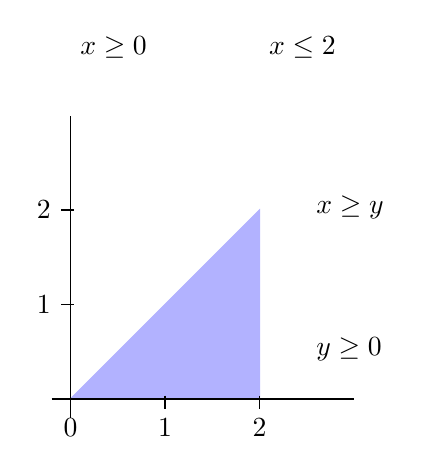
\begin{tikzpicture}[scale=1.2]

  \filldraw[color=blue!30]
    (0,0) -- (2,0) -- (2,2) -- cycle;

  \halfplane{0,0}{3,0}{+}{0.2cm}{0.8cm}
  \halfplane{0,0}{0,3}{-}{0.2cm}{1cm}
  \halfplane{2,0}{2,3}{+}{0.2cm}{1cm}
  \halfplane{0,0}{2,2}{-}{0.2cm}{2cm}
  \draw 
    (0,3.5) node[anchor=south west]{$x\ge 0$}
    (2,3.5) node[anchor=south west]{$x\le 2$}
    (2.5,1.8) node[anchor=south west]{$x\ge y$}
    (2.5,0.3) node[anchor=south west] {$y\ge 0$};



  %axis
  \draw (-.2,0) -- coordinate (x axis mid) (3,0);
  \draw (0,-.2) -- coordinate (y axis mid) (0,3);
  %ticks
  \foreach \x in {-0,...,2}
      \draw (\x,1pt) -- (\x,-3pt);
  \foreach \x in {0,...,2}
      \draw (\x,-3pt) node[anchor=north] {\x};
  \foreach \y in {1,...,2}
      \draw (1pt,\y) -- (-3pt,\y)
          node[anchor=east] {\y};

\end{tikzpicture}
\end{minipage}

\noindent
After introducing slackness variables $s_1, s_2$, we obtain a tableaux

$$
  \begin{array}{r<{ = }lll}
    f    &    &     & \phantom{-\;}y \\[1ex]\hline\rule{0mm}{3ex}
    s_1  &    & \phantom{-\;}x   & -y \\
    s_2  & 2  & -\;x
  \end{array}
$$

\noindent
for the basis  $\{s_1,s_2\}$, with the utility value  $f=0$. The only way to continue (and
reach the optimal solution with utility value $2$), is to perofrm a void pivoting step, in which 
$y$ replaces $s_1$ in the basis:
$$
  \begin{array}{r<{ = }lll}
    f    &    &  \phantom{-\;}x   & -\;s_1 \\[1ex]\hline\rule{0mm}{3ex}
    y    &    & \phantom{-\;}x   & -s_1 \\
    s_2  & 2  & -\;x
  \end{array}
$$

\noindent
A similar situation occurs quite often.

\begin{framed}
  \begin{dfn}
    A {\em void pivoting step} of a simplex algorithm is a step, in which
    the basis $B$ is transformed to $B'$ without changing the corresponding basic 
    solution.
  \end{dfn}
\end{framed}


\noindent
Void steps cannot be avoided, and as the following example from  \cite{Ch83} shows,
the algorithm may loop infinitely if we are not careful enough. Consider the following tableaux:

\begin{equation}
  \begin{array}{r<{ = }lllll}
    f    &    & \phantom{-\;} 10x_1    & -\;57x_2   &  -\;9x_3   &  -\;24x_4  \\[1ex]\hline\rule{0mm}{3ex}
    x_5  &    & -\;0.5x_1 & +\;5.5x_2  &  +\;2.5x_3 &  -\;9x_4\\
    x_6  &    & -\;0.5x_1 & +\;1.5x_2  &  +\;0.5x_3 &  -\;x_4\\
    x_7  &  1 & -\;x_1
  \end{array}
\end{equation}

\noindent
for the basis $\{x_5,x_6,x_7\}$. Suppose that this particular simplex algorithm alway selects as pivot the
variable  $x_{\mu_e}$ with the maximum value  $r_e$. If the pivoting step zeroes out several basic
variables, the algorithm selects the one with the minimal index. We leave as an exercise to verify that
the algorithm successively visits bases $\{x_1,x_6,x_7\}$, $\{x_1,x_2,x_7\}$, $\{x_2,x_3,x_7\}$, 
$\{x_3,x_4,x_7\}$, $\{x_4,x_5,x_7\}$, finally reaching the basis  $\{x_5,x_6,x_7\}$ again. 
Since we have a cycle consistnig of void steps, the algorithm will loop forever.


\noindent
Since we cannot hope to prove the convergence of the simplex method for an arbitrary choice of the pivot,
we have to fix some algorithm to select the pivot, and try to prove convergence of this algorithm.
There are many rules for the pivot selection that address the convergence issue from different approaches.
Here we shall use the so called {\em Bland's anticycleing rule}, invented  in \cite{Bland77}

\begin{framed}
  \begin{dfn}
    The {\em Bland's anticycling rule} 
    selects the pivot variable  $x_{\mu_e}$, such that  $\mu_e$ is the smallest one for which  $r_e>0$.
    If the pivoting step zeroes out several variables, the variable $x_{\beta_\ell}$ with the snmallest
    index $\beta_\ell$ leaves the basis.
  \end{dfn}
\end{framed}


\begin{veta}
  The simplex algorithm with Bland's anticycling rule always terminates and finds an optimal solution.
\end{veta}

\begin{dokaz}
We already know that if a simplex algorithm terminates the obtained solution is optimal. First note that
the only reason that may prevent a simplex algorithm from terminating is a cycle consisting solely of void steps.
Indeed, if the algorithm never terminates, it must enter the same base $B$ infinitely many times. Since any non-void
step increases the value of $f$, and the void steps don't alter it, all steps between two visits of $B$ must be void.
Hence, to prove the theorem it is sufficient to show that a cycle of void steps cannot occur.


\noindent
Let us suppose, for the sake of contradiction, that the algorithm has a tableaux for a base $B_0$, and 
succesivelly enters tableaux with bases $B_1,B_2,\ldots,B_k=B_0$, where all pivoting steps are void
(\ie all bases $B_1,\ldots,B_k$ have the same basic solution). A variable $x_i$ will be called {\em volatile}
if it appears in some basis $B_j$, but doesn't appear in another basis $B_{j'}$. Let $t$ be the maximal index such that
$x_t$ is volatile. Since $x_t$ is volatile, there is a pivoting step where $x_t$ leaves the basis, \ie
for some $j$ it holds $x_t\in B_j$ and $x_t\not\in B_{j+1}$.
So there mus exist another volatile variable $x_s$ that replaces $x_t$ in the basis:
$x_s\not\in B_j$ and $x_s\in B_{j+1}$. At the same time, however, $x_t$ must return to the basis during
the sequence $B_j,\ldots,B_k,B_1,B_2,\ldots B_{j+1}$, so there is a basis $B_{j^\star}$
such that  $x_t\not\in B_{j^\star}$ and $x_t\in B_{j^\star+1}$.
Let  $\T(B_j)$ is as follows:


\begin{equation}
  \label{LP:bland1}
\begin{array}{lllll}
  f & = & f_0 & + & \sum\limits_{k\not\in B_j} r_kx_k\\[2mm]\hline\rule{0mm}{4ex}
  x_{\beta_1} & = & p_{\beta_1} & + & \sum\limits_{k\in B_j}q_{\beta_1,k}x_k\\
    \vdots    &  & & \vdots\\
  x_{\beta_m} & = & p_{\beta_m} & + & \sum\limits_{k\in B_j}q_{\beta_m,k}x_k\\
\end{array}
\end{equation}

\noindent
where  $B_j=\{\beta_1,\ldots,\beta_m\}$. 
Since all  pivonting steps of the cycle are void by assumption, the two basis  $B_j$, and $B_{j^\star}$
have the same basic solution (\ie the values of all variables are the same). So we can write
\begin{equation}
  \label{LP:bland2}
  f = f_0 + \sum_{k=1}^nr^\star_kx_k
\end{equation}
where
$$r^\star_k=\left\{\begin{array}{ll}0&\text{if $k\in B_{j^\star}$}\\\text{coefficient $r$ by $x_k$ 
in the tableaux $\T(B_{j^\star})$}&\text{otherwise}\end{array}\right.$$
%
Since $\T(B_{j^\star})$, and in particular the equation (\ref{LP:bland2}) 
was derived by equivalent transformations from the system
(\ref{LP:bland1}), all solutions of the system
(\ref{LP:bland1}) fullfil (\ref{LP:bland2}). 
Let us now consider a solution (not necessarily basic or even feasible) of the system 
(\ref{LP:bland1}):
choose an arbitrary $y$ and set
$$
x_i=\left\{\begin{array}{ll}%
    y&\text{if $i=s$}\\
    0&\text{if $i\not=s$ and $i\not\in B_j$}\\
    p_i+q_{i,s}y&\text{if $i\in B_j$}
  \end{array}\right.
  $$
%
It is easy to see that thus constructed \bm{x} is a solution of the system  (\ref{LP:bland1})\footnote{
It is similar to performing a  pivoting step with variable  $x_s$ by the amount of $y$ without caring about
keeping the basic variables nonnegative.}
Since our \bm{x} satisfies both  (\ref{LP:bland1})  and  (\ref{LP:bland2}), be expressing $f$ in both of
them we get
$$
f_0 + r_sy = f_0 + \sum_{k=1}^nr^\star_kx_k = f_0 + r^\star_sy + \sum_{k\in B_j}r^\star_k(p_k+q_{k,s}y)
$$
which yields
$$
\left(r_s-r^\star_s-\sum_{k\in B_j}r^\star_kq_{k,s}\right)y=\sum_{k\in B_j}r^\star_kb_k
.$$
%
Since this equality holds for any $y$, and the right-hand side does not depend on $y$, it follows that
$$
r_s-r^\star_s-\sum_{k\in B_j}r^\star_kq_{k,s}=0
.$$
%
Since $x_s$ was selected pivot in the basis $B_j$, itmust hold  $r_s>0$. In  $B_{j^\star}$
the pivoting variable was  $x_t$, and since  $t>s$, it is $r^\star_s\le 0$. Further, from 
 $r_s-r^\star_s>0$ it follows that there is some $z\in B_j$ for which
$$
r^\star_zq_{z,s}>0
.$$
The variable $x_z$ is basic in $B_j$, and at the same time $z\not\in B_{j^\star}$, because $r^\star_z\not=0$.
Hence $x_z$ is volatile and by the thefinition of $t$ it holds  $z\le t$.
Moreover, $z\not=t$: since $x_t$ left the basis $B_j$ during a pivoting step, it holds 
 $q_{t,s}<0$ and  $r^\star_tq_{t,s}<0$ (since $x_t$ was pivot in  $B_{j^\star}$).
Now we see that  $z<t$. But $x_z$ was not pivot in $B_{j^\star}$, so  $r^\star_z\le0$.
Since  $r^\star_zq_z,s>0$, it must be $q_{z,s}<0$.


\noindent
From the fact that all  basic solutions in the void cycle are the same, and $z\not\in B_{j^\star}$
it folllows that  $x_z=0$  in both basic solutions  $B_j$ and  $B_{j^\star}$. 
Since  $z\in B_j$, it holds $p_z=0$.
However, that means the $x_z$ could have left the basis $B_j$, but $x_t$ was selected instead, contradicting
the Bland's anticcling rule.
\end{dokaz}

\subsection*{How to start}

\noindent
The last detail that needs to be clarified  is how the algorithm starts. So far we supposed that 
we start with a basis $B_0$ with a feasible basic solution. In the introductory example 
the starting basis $B_0$ in (\ref{simplex:eq:2}) was chosen to consist of the slackness variables
$s_1,s_2,s_3,s_4$. This approach works for programs of the form
$\max_{\bm{x}\in\R^7}\left\{ \bm{c}\tr\bm{x} \mid A\bm{x}\le\bm{b},\; \bm{x}\ge0
\right\}$ with slackness variables added, 
 if $\bm{b}\ge\bm{0}$. What about the other programs? Consider the following program:


\renewcommand{\commonii}{%
  %axis
  \draw (-0.5,0) -- coordinate (x axis mid) (1.5,0);
  \draw (0,-0.2) -- coordinate (y axis mid) (0,1.5);
  %ticks
  \foreach \x in {-0.2,-0.1,...,1.4}
      \draw (\x,1pt) -- (\x,-3pt);
  \draw (1,-3pt) node[anchor=north] {1};

  \foreach \y in {0.2,0.3,...,1.4}
      \draw (1pt,\y) -- (-3pt,\y);
  \draw (-1pt,1) node[anchor=east] {1}; 
  
  \draw (0,-3pt) node[anchor=north east]{$0$};
}


\renewcommand{\axes}{
    \draw
      (0,0,0) -- (1.5,0,0) node[anchor=north east]{$x$}
      (0,0,0) -- (0,1.5,0) node[anchor=north west]{$y$}
      (0,0,0) -- (0,0,1.5) node[anchor=south]{$s$};
}


\hspace*{-1cm}
\begin{minipage}[t]{9cm}
  \vskip 0pt
\begin{equation}
  \label{simplex-start:eq:1}
  \begin{array}{rllll}
    \text{maximize}& 4x &  & -\;z & =:  f(x,y,z)\\
  \text{subject to}& x & +\;y & +\;z & =4\\
                         & x & -\;y& & = -2\\
\multicolumn{4}{r}{x,y,z}&\ge 0
 

  \end{array}
\end{equation}
\end{minipage}
\hspace*{5mm}
\begin{minipage}[t]{5cm}
  \vskip 0pt
\tdplotsetmaincoords{70}{120}
\begin{tikzpicture}[scale=2,tdplot_main_coords]
  \axes
  \coordinate (u) at ($ (0,0,0)!2.5cm!(-1,1,0) $);
  \coordinate (v) at ($ (0,0,0)!2cm!(-1,-1,2) $);
  \coordinate (p) at ($ (1,0,0)!7mm! ($ (1,0,0)-($(u)+(v)$) $) $);
  
  \filldraw[fill=blue!30, opacity=0.3]
      (p) -- ($ (p) + (u) $) -- ($ (p) + (u) + (v) $) -- ($ (p) + (v) $) -- cycle;
  \draw[thin]
      (p) -- ($ (p) + (u) $) -- ($ (p) + (u) + (v) $) -- ($ (p) + (v) $) -- cycle;

  \filldraw[color=blue!60, fill=blue!50, opacity=0.5]
      (0.25,0.75,0) -- (0,1,0) -- (0,0.5,0.5) -- cycle;
  \filldraw[color=green!60, fill=green!90, opacity=0.2]
      (0,0.5,0) -- (0.25,0.75,0) -- (0,.5,0.5) -- cycle;
  
  \coordinate (u) at ($ (0,0,0)!1.5cm!(1,1,0) $);
  \coordinate (v) at ($ (0,0,0)!1.5cm!(0,0,1) $);
  \coordinate (p) at ($ (-0.5,0,0)!1mm! ($ (-0.5,0,0)-($(u)+(v)$) $) $);
  
  \filldraw[fill=green!30, opacity=0.3]
      (p) -- ($ (p) + (u) $) -- ($ (p) + (u) + (v) $) -- ($ (p) + (v) $) -- cycle;
  \draw[thin]
      (p) -- ($ (p) + (u) $) -- ($ (p) + (u) + (v) $) -- ($ (p) + (v) $) -- cycle;
 
  %\draw[color=red] (p) -- (-0.5,0,0);


  \filldraw[color=blue!60, fill=blue!50, opacity=0.5]
  (1,0,0) -- (0.25,0.75,0) -- (0,0.5,0.5) -- (0,0,1) -- cycle;


  \foreach \p in {(0.25,0.75,0),(0,.5,0.5)}
    \filldraw \p circle (.8pt); 
 
  \draw[very thin, dashed] 
      (0,0,0) -- (-0.74,0,0)    
      ($(-0.5,0,0)!-.1!(0.25,0.75,0)$) -- ($(-0.5,0,0)!3!(0.25,0.75,0)$)
      (0,0,0) -- (0,0,1)
      (1,0,0) -- (0,1,0) -- (0,0,1) -- cycle;
  \draw[very thick]
    (0.25,0.75,0) -- (0,0.5,0.5);

\end{tikzpicture}
\end{minipage}

\vskip 2mm
\noindent
The feasible solutions form the line segment $(1,3,0) - (0,2,2)$.
In order to start the simplex algorithm we need some feasible solution. For a given
point $(x,y,z)$ denote  $p_1:=4-x-y-z$; $p_1$ describes ``how much'' is the first equality\footnote{%
It is {\em not} the distance from $(x,y,z)$ to the plane $x+y+z=4$.} violated. Similarly,
let  $p_2:=2+x-y$  (note the equation has been rewritten in a way that the absolute term is non-negative).
Finding a feasible solution means to find a point $(x,y,z)$, such that  $p_1=p_2=0$, \ie  
$p_1,p_2\ge0$, and $p_1+p_2=0$. It is easy to see that the program  (\ref{simplex-start:eq:1})
has a feasible solution exactly when the program

\begin{equation}
  \label{simplex-start:eq:2}
  \begin{array}{rllllll}
    \text{maximize}& -\;p_1 & -\;p_2 & \\
    \text{subject to}& p_1 & &+\;x & +\;y & +\;z & =4\\
                           & & p_2 & -\;x& +\;y & & = 2\\
\multicolumn{6}{r}{x,y,z,p_1,p_2}&\ge 0
 

  \end{array}
\end{equation}

\noindent
has a feasible solution with value $0$.
In this case it is easy to check that  $\{p_1,p_2\}$ is the basis of the feasible solution.
So we can use the simplex algorithm to find optimum of the second program, and use it as a starting
point of the original program.

\noindent
This approach can be used always. Let us consider a linear program in the normal form
$$ \max_{\bm{x}\in\R^n}\left\{ \bm{c}\tr\bm{x} \mid A\bm{x}=\bm{b},\;\bm{x}\ge\bm{0}\right\}$$


\noindent
First make sure that  $\bm{b}\ge0$: if $b_i<0$ for some $i$, premultiply the corresponding equation 
by $-1$. Introduce new variables  $x_{n_1},\ldots,x_{n+m}$  and set up the auxiliary program
$$ \max_{\tilde{\bm{x}}\in\R^{n+m}}\left\{ -x_{n+1}-\ldots-x_{n+m} \mid \tilde{A}\tilde{\bm{x}}=\bm{b},\;\tilde{\bm{x}}\ge\bm{0}\right\}$$
where $\tilde{A}=(A\mid I_m)$ is obtained from $A$ by augmenting with identity matrix of dimensions $m\times m$.
Since  $\bm{b}\ge0$, $\{x_{n+1},\ldots,x_{n+m}\}$ form a basis of a feasible solution, and simplex algorithm can be used
to compute the optimum. If the value optimum is 0, we got a feasible solution of the original program. 
On the other hand, for any feasible solution of the original program there is a solution of the auxiliary program with value 0. Hence, if the optimum of the auxiliary program is not 0, the original program had no feasible solution.

\begin{prob}
  Implement the simplex algorithm with Bland's anticycling rule.
\end{prob}

% % % % % % % % % % % % % % % % % % % % % % % % % % % % % % % % % % % % % % % %
\section{Complexity of the simplex algorithm}

\noindent
In the last chapter we introduced the simplex method for solving linear programs in a more efficient way
than to check all the vertices of the polyhedron of feasible solutions. We showed that the simple method
with the Bland's anticycling rule always terminates. Now the question is how efficient it is. 
Surprisingly enough, inspite of the fact that the simplex algorithm works very well in practice,
its worst-case complexity is exponential as we show in a minute.


\noindent
Before doing so, let us review some basic facts, as the subtle details will play a significant role here.
When analyzing the complexity of an algorithm, we do so with respect to some parameter that is, in general,
a part of the definition of the problem. When e.g. we say that the algorithm has complexity $O(n^2)$,
we mean that there is a constant $c$ and some $n_0$ such that for any input with the parameter
$n>n_0$ the running time of the algorithm is at most $cn^2$. A natural and universally available parameter
is the length of the input: the definition of the problem always contains the description of how the input is
represented as a binary string and the length (number of bits) of this string is a good complexity parameter.
Sometimes (and actually quite often), however, we use different parameters that are more natural for the problem:
e.g. when analyzing sorting algorithms, the parameter is usually tne number of the numbers to be sorted, although
the length of the input depends also on the sizes of the numbers. Similarly, in graph algorithms we sometimes
use the number of vertices as the parameter, although $\Omega(n^2)$ bits are needed 
to represent a graph with $n$ vertices
\footnote{It is sufficient to note that a labeled graph may contain up to  ${n\choose 2}$, and each of then 
  may be present in the graph or not, so there are $2^{n\choose 2}$ (labelled) graphs, and so using the
pidgeon-hole principle we need at least $n\choose 2$ bits to identify them.}

\noindent
The instance of a linear program with $n$ variables and $m$ constraints consists of two vectors of real numbers
\bm{c} and \bm{b}, and a matrix  $A\in\R^{m\times n}$. Natural complexity parameters would be $m$, $n$, or the
length of the input, where in the latter case we need to specify the encoding of the reals, and accept the
fact that if we want to have finite inputs, we cannot encode all  real numbers.

\noindent
These details should be kept in mind, although we are not really worrying about them now: we shall construct an 
input with $n$ variables and $2n$ constraints where the simplex algorithm performs $\Omega(2^n)$ iterations.
Moreover, we shall use only numbers with short description (actually, only the numbers  
$\{\pm1,\pm\frac{1}{4},0\}$), so we show exponential complexity in any of the abovementioned parameters.

\noindent
Consider the simplex algorithm with the Bland's anticycleing rule (for a number of other pivot-choosing
strategies there are similar proofs available). We construct, for each $n$, an input instance with $n$ variables
and $2n$ constraints in such a way that the polyhedron of feasible solutions has $2^n$ vertices
and the simplex algorithm visits all of them. In our instance the goal is to maximize the variable $x_n$,
and the constraints form a skewed cube. Let us begin by creating an $n$-dimensional cube using
$2n$ constraints:
$$
\begin{array}{rll}
  0\le &x_1& \le 1\\
  0\le &x_2& \le 1\\
  \multicolumn{3}{c}{\cdots}\\
  0\le &x_n& \le 1
\end{array}
$$

\noindent
In three dimensions the polyhedron of the feasible solutions is a cube:
\renewcommand{\common}{
    \draw[->,thin]
      (1,0,0) -- (1.2,0,0) node[anchor=north east]{$x$};
    \draw[->,thin]
      (0,1,0) -- (0,1.2,0) node[anchor=north west]{$y$};
    \draw[->,thin]
      (0,0,1) -- (0,0,1.2) node[anchor=south]{$z$};

}

\newcommand{\tmpNode}[2]{
  (#1) circle (.5pt) node[anchor=#2] {\footnotesize $(#1)$}
}

\begin{center}
  \tdplotsetmaincoords{70}{120}
  \begin{tikzpicture}[scale=3,tdplot_main_coords]
      \draw[dashed]
        (0,0,0) -- (1,0,0)
        (0,0,0) -- (0,1,0)
        (0,0,0) -- (0,0,1);
    

    %\fill[fill=blue!20]
    %  (6,0,0) -- (5,4,0) -- (1,0,4);

    \draw
    (1,0,0) -- (1,1,0) -- (0,1,0) -- (0,1,1) -- (1,1,1) -- (1,0,1) -- (0,0,1) -- (0,1,1)
    (1,0,0) -- (1,0,1)
    (1,1,0) -- (1,1,1)
    ;

    \common
    \filldraw
    \tmpNode{1,0,0}{south east}
    \tmpNode{0,1,0}{south west}
    \tmpNode{0,0,1}{south west}
    \tmpNode{0,1,1}{south west}
    \tmpNode{0,1,0}{south west}
    \tmpNode{1,0,1}{east}
    \tmpNode{1,1,0}{north}
    \tmpNode{1,1,1}{north west}
    \tmpNode{0,0,0}{south east}

    ;
    
  \end{tikzpicture}
\end{center}


\noindent
Now we want to shift the vertices such that there is a long increasing spiral.
Choose some $\varepsilon<\frac{1}{2}$ and define constraints:

$$
\begin{array}{rll}
  \varepsilon\le &x_1& \le 1\\
  \varepsilon x_1\le &x_2& \le 1-\varepsilon x_1\\
  \multicolumn{3}{c}{\cdots}\\
  \varepsilon x_{n-1}\le &x_n& \le 1-\varepsilon x_{n-1}
\end{array}
$$

Transform the program into the normal form by introducing slackness variables $r_i, s_i$
so that the constraints are expressed as equalities. This yields a program:
\begin{equation}
\label{eq:simplex:exp:1}
\begin{array}{ll}
  \text{maximize} & x_n\\
  \vtop{\null\hbox{\text{subject to}}} & \vtop{\null\hbox{$\begin{array}{rl}
  x_1-r_1 &=\varepsilon\\
  x_1+s_1 &=1\\
  x_2 - \varepsilon x_1 - r_2 &=0\\
  x_2 + \varepsilon x_1 + s_2 &=1\\
  \cdots&\cdots\\
  x_n - \varepsilon x_{n-1} - r_n &=0\\
  x_n + \varepsilon x_{n-1} + s_n &=1
\end{array}$}}\\
\end{array}
\end{equation}
where all variables are non-negative. How do the feasible basic solutions look like?
Thanks to the slackness variables, the constraints are linearly independent (each constraint
contains a variable that does not appear anywhere else), so the basis has $2n$ elements.
Moreover, $r_1+s_1=1-\varepsilon$ , and for each pair of variables $r_i, s_i$
where $i>1$ it holds  $r_i+s_i=1-2\varepsilon x_{i-1}>0$.  Hence, it cannot hold  $r_i=s_i=0$,
and so each basis must contain at least one of the variables $r_i, s_i$.
Still more, all  $x_i>0$, and so they appear in every basis. Each basis $B$ is thus uniquely
characterized by a set  $R_B\subseteq\{1,\ldots,d\}$: basic variables are 
$$\{x_1,\ldots,x_n\}\cup\bigcup\limits_{i\in R_B}\{r_i\}\cup\bigcup\limits_{i\not\in R_B}\{s_i\}$$ 


\noindent
At the same time, the following claim is obvious:
\begin{clm}
  \label{clm:simplex:exp:1}
  Each pivoting step is uniquely characterized by an index $i$. The step changes the 
  membership in the basis for variables  $r_i$ and $s_i$.
\end{clm}

\noindent
To illustrate the program, let $n=3$. In the matrix notation, the program is 
$$\max\{x_3\mid A\bm{x}=\bm{b}, \bm{x}\ge 0\}$$
where
\begin{align*}
  A&=\left(\begin{array}{ccccccccc}
  1&0&0&-1&0&0&0&0&0\\
  1&0&0&0&1&0&0&0&0\\
  -\varepsilon&1&0&0&0&-1&0&0&0\\
  \varepsilon&1&0&0&0&0&1&0&0\\
  0&-\varepsilon&1&0&0&0&0&-1&0\\
0&\varepsilon&1&0&0&0&0&0&1\end{array}\right) &
\bm{x}&=\left(\begin{array}{l}x_1\\x_2\\x_3\\r_1\\s_1\\r_2\\s_2\\r_3\\s_3\end{array}\right) &
\bm{b}&=\left(\begin{array}{l}\varepsilon\\1\\0\\1\\0\\1\end{array}\right)
\end{align*}

\noindent
The matrix $A$ has rank $6$, and $R_B\subseteq\{1,2,3\}$. So there are $6$ basic solutions
that form a skewed cube:


\begin{center}
  \renewcommand{\tmpNode}[3]{
    (#1) circle (.5pt) node[anchor=#2] {\footnotesize $(#3)$}
  }
  \newcommand{\ee}{0.2}
  \vskip 0pt
  \tdplotsetmaincoords{70}{120}
  \begin{tikzpicture}[scale=4.5,tdplot_main_coords]

    %\fill[fill=blue!20]
    %  (6,0,0) -- (5,4,0) -- (1,0,4);

    \draw[dotted,color=blue]
    (1,0,0) -- (1,1,0) -- (0,1,0) -- (0,1,1) -- (1,1,1) -- (1,0,1) -- (0,0,1) -- (0,1,1)
    (1,0,0) -- (1,0,1)
    (1,1,0) -- (1,1,1)
        (0,0,0) -- (1,0,0)
        (0,0,0) -- (0,1,0)
        (0,0,0) -- (0,0,1);
    
    ;

    \common
   
    %\draw[thin,dotted,color=blue]
    %(1,0,0) -- (1,\ee,0) -- (1,\ee,\ee*\ee)
    %;

    \draw
      (\ee,\ee*\ee,\ee*\ee*\ee) -- (1,\ee,\ee*\ee) -- (1,1-\ee,\ee-\ee*\ee) -- (\ee,1-\ee*\ee,\ee-\ee*\ee*\ee) 
      -- (\ee,1-\ee*\ee,1-\ee+\ee*\ee*\ee) 
      -- (1,1-\ee,1-\ee+\ee*\ee) -- (1,\ee,1-\ee*\ee) -- (\ee,\ee*\ee,1-\ee*\ee*\ee)
      (1,\ee,\ee*\ee) -- (1,\ee,1-\ee*\ee)
      (1,1-\ee,\ee-\ee*\ee)--(1,1-\ee,1-\ee+\ee*\ee)
      (\ee,\ee*\ee,1-\ee*\ee*\ee) -- (\ee,1-\ee*\ee,1-\ee+\ee*\ee*\ee)
    ;

    \draw[dashed]
    (\ee,\ee*\ee,\ee*\ee*\ee) -- (\ee,\ee*\ee,1-\ee*\ee*\ee)
    (\ee,\ee*\ee,\ee*\ee*\ee) --  (\ee,1-\ee*\ee,\ee-\ee*\ee*\ee)
    ;

    \draw[thick,color=red,->]
      (\ee,\ee*\ee,\ee*\ee*\ee) -- (1,\ee,\ee*\ee) -- (1,1-\ee,\ee-\ee*\ee) -- (\ee,1-\ee*\ee,\ee-\ee*\ee*\ee) 
      -- (\ee,1-\ee*\ee,1-\ee+\ee*\ee*\ee) 
      -- (1,1-\ee,1-\ee+\ee*\ee) -- (1,\ee,1-\ee*\ee) -- (\ee,\ee*\ee,1-\ee*\ee*\ee)
    ;

    \filldraw
    \tmpNode{\ee,\ee*\ee,\ee*\ee*\ee}{south east}{\varepsilon,\varepsilon^2,\varepsilon^3}
    \tmpNode{1,\ee,\ee*\ee}{south east}{1,\varepsilon,\varepsilon^2}
    \tmpNode{1,1-\ee,\ee-\ee*\ee}{north west}{1,1-\varepsilon,\varepsilon-\varepsilon^2}
    \tmpNode{\ee,1-\ee*\ee,\ee-\ee*\ee*\ee}{south west}{\varepsilon,1-\varepsilon^2,\varepsilon-\varepsilon^3}
    \tmpNode{\ee,1-\ee*\ee,1-\ee+\ee*\ee*\ee}{south west}{\varepsilon,1-\varepsilon^2,1-\varepsilon+\varepsilon^3}
    \tmpNode{1,1-\ee,1-\ee+\ee*\ee}{north west}{1,1-\varepsilon,1-\varepsilon+\varepsilon^2}
    \tmpNode{1,\ee,1-\ee*\ee}{east}{1,\varepsilon,1-\varepsilon^2}
    \tmpNode{\ee,\ee*\ee,1-\ee*\ee*\ee}{south east}{\varepsilon,\varepsilon^2,1-\varepsilon^3}
    ;
  \end{tikzpicture}
\end{center}
\noindent
The red edges correspond to an increasing path starting in the solution with the set  $R_{B_0}=\emptyset$,
and going through all vertices. The path always moves in the first dimension in which the utility function grows. 
In order to generalize this example to $n$ dimensions we need to be able to reason about the pivoting
steps of the algorithm with Bland's anticycling rule. This can be done using the claim~\ref{clm:simplex:exp:1}
and the following lemma:


\begin{lema}
  \label{lm:simplex:exp:1}
  Given a basis $B$ of the program~(\ref{eq:simplex:exp:1}), with the corresponding tableaux $\T(B)$,
  let the utility function in $\T(B)$ be expressed in terms of non-basic variables as 
  $x_n=c_0+c_1v_1+c_2v_2+\cdots+c_nv_n$, where  $v_i$  is either $r_i$ or  $s_i$, and $c_i$ is the
  corresponding
  coefficient. Then $c_i$ is positive exactly if the number of basic variables $r_j$ for $j\ge i$ is
  even, \ie
  $$\left|\{j\mid j\in R_B,\;j\ge i\}\right|\equiv 0\; (\mod 2)$$
\end{lema}

\begin{dokaz}
  The proof is done by induction on the dimension of the problem $n$. For $n=1$, if $r_1$ is in the
  basis we get  $x_1=1-s_1$ and $c_1$ is negative, and if $r_1$ is not in the basis, then $x_1=\varepsilon+r_1$ 
  and $c_1$ is positive.

  \noindent
  Now suppose the statement holds for $n-1$. If $n\in R_B$, the expression for $x_n$ must
  contain $s_n$, and hence must be of the form $x_n=1-s_n-\varepsilon (c_0'+c_1'v_1'+\cdots+c_{n-1}'v_{n-1}')$,
  where $x_{n-1}=c_0'+c_1'v_1'+\cdots+c_{n-1}'v_{n-1}'$ is expressed in the non-basic variables
  $v_1,\ldots,v_{n-1}$. The result follows by expanding and applying the induction hypothesis.
  If $n\not\in R_B$, the approach is similar using the equality $x_n=r_n+\varepsilon x_{n-1}$.
\end{dokaz}

\noindent
Now we can show that the simplex algorithm visits all vertices:

\begin{veta}
  Let $i\in\{1,\ldots,n\}$ and 
  $R\subseteq\{i+1,\ldots,n\}$. 
  If the simplex algorithm with the Bland's anticycling rule starts in a basis $B_0$ with
  $R_{B_0}=R$ 
  (resp. $R_{B_0}=\{i\}\cup R$) and $|R|$ is even (resp. $|R|$ is odd),
  it visits all the bases of the form  $R'\cup R$ where $R'\subseteq\{1,\ldots,i\}$, and
  terminates in a basis $B_1$ with $R_{B_1}=\{i\}\cup R$ (resp. $R_{B_1}=R$).
\end{veta}

\begin{dokaz}
  The proof is by induction on $i$. If $i=1$ then in both cases ($R_{B_0}=R$, $|R|$ even, 
  and  $R_{B_0}=\{1\}\cup R$, $|R|$ odd) Lemma~\ref{lm:simplex:exp:1} asserts that the coefficient
  at $v_1$ is positive, and the algorithm performs a pivoting step with index $1$.

  \noindent
  Now let the statement hold for $i-1$. There are two cases. First, let  $R_{B_0}=R$ with $|R|$ even.
  Since  $R\subseteq\{i,\ldots,n\}$ we can use the induction hypothesis: the algorithm visits all bases
  of the form $R'\cup R$ where $R'\subseteq\{1,\ldots,i-1\}$, and terminates in  $\{i-1\}\cup R$.
  Since $|R|$ is even, according to Lemma~\ref{lm:simplex:exp:1} the algorithm enters the basis
  $\{i-1,i\}\cup R$. The induction hypothesis for $i-1$ and an odd set $\{i\}\cup R$ yields the result.

  \noindent
  The second case where $R_{B_0}=\{i\}\cup R$, and $|R|$ is odd can be taken care of in a similar fashion,
  and we leave it to the reader.
\end{dokaz}

\begin{dosl}
  The simplex algorithm with Bland's anticycling rule performs exponentially many iterarions on the
  program
  (\ref{eq:simplex:exp:1}).
\end{dosl}


\noindent
Now we can see that the simplex algorithm is exponential in the worst case regardless of whether the 
complexity parameter is the number of variables, the number of constraints, or the length of the input. 
How come then it performs so well in practical situations? One possible attempt in explaining it, is to 
analyze the average case. However, there is an immediate problem -- how to define the ''average'' case.
Indeed, there are results stating that the simplex algorithm performs polynomially many iterations in the
average case, where the ''average case'' is the expected number of iterations if both the matrix $A$, and
the vectors \bm{c}, \bm{b} are selected at random from a given probability distribution.
However, this is not very satisfying answer: the average case defined this way is actually very far
from a ''typical'' case that is solved in practice, where the (matrices of the) programs usually exhibit
a great deal of structure. An interesting explanation was found using the notion of {\em smoothed complexity}
that combines the worst case and the average case analysis. 
It considers all instances (\ie worst-case), but for each instance we analyze the expected time over all
instances that are ''close'' enough - \ie those that can be obtained using some small perturbation. 
Spielman and Teng \cite{ST04} showed that the smoothed complexity of the simplex algorithm is polynomial.
If we  imagine the space of all solutions as a plane, the comlexity of the simplex algorithm looks like the
picture on the left -- it is usually polynomial, with sparsely spaced ''bad'' instances.


\centerline{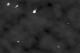
\includegraphics[width=0.65\textwidth]{smoothed/smoothed-A.pdf}\hspace*{-2cm}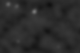
\includegraphics[width=0.65\textwidth]{smoothed/smoothed-B.pdf}}

\noindent
After averaging over small neighbourhoods, the bad instances are smoothed as on the right picture. 
This explains why the simplex method can be considered efficient even if it is not polynomial in the
strict sense: in order to come up with an superpolynomial-time instance, the values must be set very
precisely; any small random perturbation of the values yields an instance with polynomial solution.

\noindent
The result of Spielman and Teng is considered a breakthrough an on the first (and second, and third) 
sight may seem as magic. It is out of the scope of this text to present the complete proof, but we
would like to finish this chapter with a simple visual reasoning why it might actually work.


\noindent
In the previous text we introduced the simplex algorithm with the Bland's anticycling rule. This time, however,
the analysis is done using a different rule, called {\em shadow tracing}. Let's have a linear program in the
form
$$\max_{\bm{x}\in\R^n}\{\bm{c}\tr\bm{x}\mid A\bm{x}\le\bm{b},\bm{x}\ge0\}$$
The feasible soluitons form a polyhedron $\cal D$ in an $n$-dimensional space, and to find an optimal basic
solution means to find a vertex $\cal D$ that is furthest in the direction of the vector \bm{c}.
Since we know that in two dimensions, this prolblem is easy, we can reason as follows:
let's have a starting basic solution $\bm{x_0}$. Since it is a vertex of $\cal D$,
there is a vector \bm{alpha} such that the vertex $\bm{x_0}$ maximizes the value 
$\bm{\alpha}\tr\bm{x}$ ($\bm{x_0}$ is farthest in the direction of \bm{\alpha}).
Take the (2-dimensional) plane spanned by the vectors \bm{\alpha} and \bm{c}, and 
project every vertex of $\cal D$ into it. We get a set of points in the plane, and their convex hull is
the {\em shadow} that $\cal D$ casts into the plane.

\vskip 1ex
\noindent
\newcommand{\faceT}[3]{\draw[face] (v#1) -- (v#2) -- (v#3) -- cycle; }
\newcommand{\faceQ}[4]{\draw[face] (v#1) -- (v#2) -- (v#3) -- (v#4) -- cycle; }
\newcommand{\faceP}[5]{\draw[face] (v#1) -- (v#2) -- (v#3) -- (v#4) -- (v#5) -- cycle; }
\newcommand{\faceS}[6]{\draw[face] (v#1) -- (v#2) -- (v#3) -- (v#4) -- (v#5) -- (v#6) -- cycle; }

\newcommand{\tmpvec}[4]{
    \draw[thick,red,->]
    (#1) -- coordinate (mid) ($ (#1) + (#2) $);
    \draw[fill=black] (#1) circle (0.6pt) node [below=4pt, black] {#3};
    \node [anchor=south,red] at (mid) {#4};

  }


\begin{center}
  \tdplotsetmaincoords{80}{10}
  \begin{tikzpicture}[scale=2.3,tdplot_main_coords]

    \coordinate (v1) at ( 0.098148, 1.315036,  0.627859);
    \coordinate (v2) at ( 1.348569, -0.000557,  0.425867);
    \coordinate (v3) at ( -1.289792, -0.534572,  -0.650170);
    \coordinate (v4) at ( 0.906291, -1.260214,  -0.285596);
    \coordinate (v5) at ( 0.862122, 0.955805,  0.706217);
    \coordinate (v6) at ( -0.997535, -1.073127,  -0.802253);
    \coordinate (v7) at ( 1.162205, -0.994616,  -0.084187);
    \coordinate (v8) at ( -1.263039, 0.086707,  -0.359741);
    \coordinate (v9) at ( -0.503439, -1.342548,  -0.768410);
    \coordinate (v10) at ( -0.680657, 0.849360,  0.170420);
    \coordinate (v11) at ( 0.060013, 0.461626,  0.673989);
    \coordinate (v12) at ( 0.791863, -0.308369,  0.555766);
    \coordinate (v13) at ( -0.752325, -0.620919,  -0.074020);
    \coordinate (v14) at ( 0.533005, -1.045626,  0.139359);
    \coordinate (v15) at ( 0.507154, 0.251374,  0.719851);
    \coordinate (v16) at ( -0.581272, -0.936126,  -0.163032);
    \coordinate (v17) at ( 0.682788, -0.890175,  0.257240);
    \coordinate (v18) at ( -0.736667, -0.257295,  0.095963);
    \coordinate (v19) at ( -0.292086, -1.093814,  -0.143224);
    \coordinate (v20) at ( -0.395809, 0.189073,  0.406257);
    \coordinate (v21) at ( 0.055710, -0.078977,  0.550938);
    \coordinate (v22) at ( 0.289348, -0.384593,  0.486054);
    \coordinate (v23) at ( -0.420460, -0.528261,  0.196564);
    \coordinate (v24) at ( 0.204785, -0.687756,  0.321740);
    \coordinate (v25) at ( -0.275369, -0.709392,  0.160201);
    \coordinate (v26) at ( -0.256582, -0.155937,  0.417331);
    \coordinate (v27) at ( 0.397235, -0.149936,  -0.400718);
    \coordinate (v28) at ( 0.615677, -0.244497,  -0.374613);
    \coordinate (v29) at ( 0.243147, -0.354227,  -0.542127);
    \coordinate (v30) at ( 0.604557, -0.495540,  -0.492066);
    \coordinate (v31) at ( 0.325407, -0.508119, -0.585981 );

    \def\bot{-1.5}
    
    \coordinate (w1) at ( 0.098148, 1.315036, \bot );
    \coordinate (w2) at ( 1.348569, -0.000557, \bot );
    \coordinate (w3) at ( -1.289792, -0.534572, \bot );
    \coordinate (w4) at ( 0.906291, -1.260214, \bot );
    \coordinate (w5) at ( 0.862122, 0.955805, \bot );
    \coordinate (w6) at ( -0.997535, -1.073127, \bot );
    \coordinate (w7) at ( 1.162205, -0.994616, \bot );
    \coordinate (w8) at ( -1.263039, 0.086707, \bot );
    \coordinate (w9) at ( -0.503439, -1.342548, \bot );
    \coordinate (w10) at ( -0.680657, 0.849360, \bot );
    \coordinate (w11) at ( 0.060013, 0.461626, \bot );
    \coordinate (w12) at ( 0.791863, -0.308369, \bot );
    \coordinate (w13) at ( -0.752325, -0.620919, \bot );
    \coordinate (w14) at ( 0.533005, -1.045626, \bot );
    \coordinate (w15) at ( 0.507154, 0.251374, \bot );
    \coordinate (w16) at ( -0.581272, -0.936126, \bot );
    \coordinate (w17) at ( 0.682788, -0.890175, \bot );
    \coordinate (w18) at ( -0.736667, -0.257295, \bot );
    \coordinate (w19) at ( -0.292086, -1.093814, \bot );
    \coordinate (w20) at ( -0.395809, 0.189073, \bot );
    \coordinate (w21) at ( 0.055710, -0.078977, \bot );
    \coordinate (w22) at ( 0.289348, -0.384593, \bot );
    \coordinate (w23) at ( -0.420460, -0.528261, \bot );
    \coordinate (w24) at ( 0.204785, -0.687756, \bot );
    \coordinate (w25) at ( -0.275369, -0.709392, \bot );
    \coordinate (w26) at ( -0.256582, -0.155937, \bot );
    \coordinate (w27) at ( 0.397235, -0.149936, \bot );
    \coordinate (w28) at ( 0.615677, -0.244497, \bot );
    \coordinate (w29) at ( 0.243147, -0.354227, \bot );
    \coordinate (w30) at ( 0.604557, -0.495540, \bot );
    \coordinate (w31) at ( 0.325407, -0.508119, \bot );
    
    \draw[black] (-2,-2,\bot) -- (2,-2,\bot) -- (2,2,\bot) -- (-2,2,\bot) -- cycle;
    
    \draw[black,fill=gray!80, fill opacity=0.8] (w1)
      \foreach \i in {5,2,7,4,9,6,3,8,10}
      { -- (w\i) }
      -- cycle;

    \foreach \i in {1,...,31}
    \draw[black!30!green,dotted, fill=black] (v\i) circle (.3pt) 
    %node [black,anchor=north] {\tiny \i}
    -- (w\i) circle (.3pt) 
    %node [black,anchor=north] {\tiny \i}
    ;

    

    \IGNORE{
    \draw[blue,thick] (0,0,0) -- (0,0,1.2) node {z}
    (0,0,0) -- (0,1.2,0) node {y}
    (0,0,0) -- (1.2,0,0) node {x};
    }

 %invisible   
    \tikzset{face/.style = {black, dashed, very thin}}
    
    \faceP{30}{31}{29}{27}{28}
    \faceQ{10}{1}{11}{20}
    \faceQ{27}{29}{8}{10}
    \faceT{27}{1}{10}
    \faceT{29}{3}{8}
    \faceQ{31}{29}{3}{6}
    \faceQ{30}{28}{2}{7}
    \faceQ{1}{5}{28}{27}
    \faceT{28}{2}{5}
    \faceT{31}{6}{9}
    \faceT{30}{4}{7}

 % visible
    \tikzset{face/.style = {black!90!blue, very thin, fill=yellow!80,fill opacity=0.4}}

    \faceQ{31}{30}{4}{9}
    
    \faceQ{5}{1}{11}{15}
    \faceQ{5}{2}{12}{15}
    \faceQ{7}{4}{14}{17}
    \faceQ{9}{4}{14}{19}
    \faceQ{9}{6}{16}{19}
    \faceQ{7}{2}{12}{17}
    \faceQ{6}{3}{13}{16}
    \faceQ{8}{3}{13}{18}
    \faceQ{20}{18}{23}{26}
    \faceQ{10}{8}{18}{20}
    \faceT{18}{13}{23}
    \faceQ{16}{13}{23}{25}
    \faceT{19}{16}{25}
    \faceQ{19}{14}{24}{25}
    \faceT{17}{14}{24}
    \faceQ{17}{12}{22}{24}
    \faceQ{15}{12}{22}{21}
    \faceQ{20}{11}{21}{26}
    \faceT{15}{11}{21}
    \faceS{24}{25}{23}{26}{21}{22}
   
    \def\len{0.6}
    \tmpvec{v3}{-\len,-\len,0}{$\bm{x_0}$}{$\bm{\alpha}$}
    \tmpvec{w3}{-\len,-\len,0}{ }{ }
    \tmpvec{v2}{\len,0,0}{$\;\;\bm{x^\star}$}{$\bm{c}$}
    \tmpvec{w2}{\len,0,0}{ }{ }

    \draw[thick,fill=black] (v3)
    \foreach \i in {6,9,4,7,2}
    { circle (0.6pt) -- (v\i) }
    circle(0.6pt);
    
    \draw[thick,fill=black] (w3)
    \foreach \i in {6,9,4,7,2}
    { circle (0.6pt) -- (w\i) }
    circle(0.6pt);

    \draw (-.6,-.6,.6) node {\LARGE $\cal D$};

  \end{tikzpicture}
\end{center}



\noindent
It is not difficult to see that the projections of both  $\bm{x_0}$, and the optimal solution  $\bm{x^\star}$
are located on the boundary of the shadow. A simplex algorithm with the shadow vertex rule 
always selects during a pivoting step a basic solution whose projection  is on the boundary of the shadow. 
This can be tested
e.g. by considering all possible pivoting steps, and comparing their projections (although more efficient
ways exist). The number of iterations is clearly upper-bounded by the number of 
the number of points that project to the shadow boundary. An important step in the proof is to transform
the program to the form where the constraints are of the form $\bm{a_i}\tr\bm{x}\le1$;
in this case there is a polar description of $\cal D$, and it can be observed that the number of the
vertives of the shadow is at most the number of vertices of a polynome $\cal M$, which is formed
as an intersection of the conver hull of points $\bm{a_1},\ldots,\bm{a_n}$ with the plane spanned
by vectors $\bm{\alpha}$, $\bm{c}$.
The core of the proof is a geometric statemet: given $n$ points in a $d$-dimensional space, if each 
of them is translated by a random vector with normal distribution, then in the expected case 
the corresponding polymone $\cal M$ has at most $poly(n,d,\frac{1}{\sigma})$ points, where $\sigma^2$
is the standard deviation.

\noindent
It is still a long way to the actual proof; we only wanted to hint on the direction to make the result more
believable. Interested readers are invited to look into the paper [Spielman, Teng]. or the 
lecture notes
{\tt http://www.cs.yale.edu/homes/spielman/BAP/}

\chapter{Rounding of linear programs}
\section{Integer programs and relaxation: the good, the bad, and the ugly}
\label{sec-ilp}

\noindent 
In the previous parts we showed how the linear programming problem can be solved efficiently.
In solving real-life problems, we are often interested only in solutions where some of the 
variables involved are forced to be integers. In the first motivation example we found out
that the optimal solution is to buy $2\frac{2}{3}$ dl of green stuff. This would probably not
be feasible, since drinks are usually served in multiples of some fixed volume. 


\begin{center}
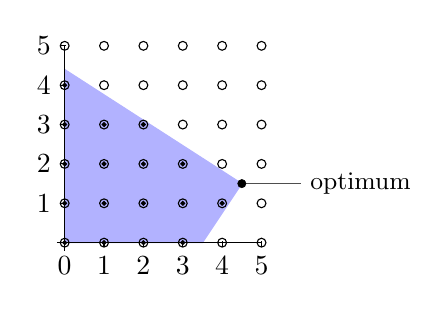
\begin{tikzpicture}[scale=0.5]

  \filldraw[color=blue!30]
  (0,0) -- (3.5,0) -- (4.5,1.5) -- (0,4.4) -- cycle;

  \halfplane{0,0}{5,0}{+}{0.5cm}{0.8cm}
  \halfplane{3.5,0}{4.5,1.5}{+}{0.2cm}{2.4cm}
  \halfplane{0,4.4}{4.5,1.5}{-}{0.5cm}{2.4cm}
  \halfplane{0,0}{0,5}{-}{0.5cm}{1cm}

  %\draw 
  %  (0,3.5) node[anchor=south west]{$x\ge 0$}
  %  (2,3.5) node[anchor=south west]{$x\le 2$}
  %  (2.5,1.8) node[anchor=south west]{$x\ge y$}
  %  (2.5,0.3) node[anchor=south west] {$y\ge 0$};


  \draw
    \foreach \x in {0,...,5}
      \foreach \y in {0,...,5}
      {(\x,\y) circle (3.2pt)};

  \filldraw
  \foreach \x in {0,...,2}
      \foreach \y in {0,...,2}
      {(\x,\y) circle (1.4pt)};
  
  \filldraw   
  \foreach \p in {(0,3),(0,4),(1,3),(3,2),(3,1),(4,1),(2,3),(3,0)}
      {\p circle (1.4pt)};

  %axis
  \draw (-.2,0) -- coordinate (x axis mid) (5,0);
  \draw (0,-.2) -- coordinate (y axis mid) (0,5);
  %ticks
  \foreach \x in {-0,...,5}
      \draw (\x,1pt) -- (\x,-3pt);
  \foreach \x in {0,...,5}
      \draw (\x,-3pt) node[anchor=north] {\x};
  \foreach \y in {1,...,5}
      \draw (1pt,\y) -- (-3pt,\y)
          node[anchor=east] {\y};

  \filldraw[very thin]
    (4.5,1.5) circle (3pt)
    (6,1.5) -- (4.5,1.5)
    (6,1.5) node[anchor=west] {{\small optimum}};

    
\end{tikzpicture}
\mycaption{Feasible solutions of a linear program and its integral restriction.}
\end{center}

\noindent 
The first intuition might suggest that this is just a small technical issue: after all, we can always find the 
optimal solution of the continuous version, round it in some way and get, if not the optimal solution, then 
surely something reasonably close to the optimum. On a second thought one starts wondering that it might not be
so easy: if a linear program  used to find out whether to travel by air or by train
recommends to buy half air and half train ticket, the rounding is as complex as the entire solution. The following 
picture shows that the closest integer solution might be quite far from the optimum, and it is not obvious how to
find it. 

\begin{center}
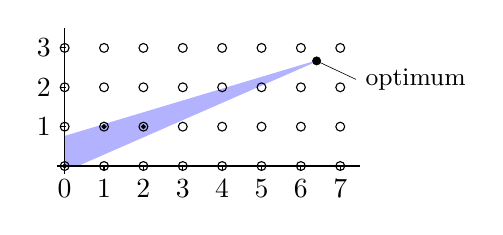
\begin{tikzpicture}[scale=0.5]

  \filldraw[color=blue!30]
  (0,0) -- (0.3,0) -- (6.4,2.67) -- (0,0.75) -- cycle;

  \halfplane{0,0}{7,0}{+}{0.5cm}{0.8cm}
  \halfplane{0.3,0}{6.4,2.67}{+}{0.2cm}{2.4cm}
  \halfplane{0,0.75}{6.4,2.67}{-}{0.5cm}{2.4cm}
  \halfplane{0,0}{0,3}{-}{0.5cm}{1cm}



  \draw
    \foreach \x in {0,...,7}
      \foreach \y in {0,...,3}
      {(\x,\y) circle (3.2pt)};

  \filldraw   
  \foreach \p in {(0,0),(1,1),(2,1)}
      {\p circle (1.4pt)};

  %axis
  \draw (-.2,0) -- coordinate (x axis mid) (7.5,0);
  \draw (0,-.2) -- coordinate (y axis mid) (0,3.5);
  %ticks
  \foreach \x in {-0,...,7}
      \draw (\x,1pt) -- (\x,-3pt);
  \foreach \x in {0,...,7}
      \draw (\x,-3pt) node[anchor=north] {\x};
  \foreach \y in {1,...,3}
      \draw (1pt,\y) -- (-3pt,\y)
          node[anchor=east] {\y};

  \filldraw[very thin]
    (6.4,2.67) circle (3pt)
    (7.4,2.2) -- (6.4,2.67)
    (7.4,2.2) node[anchor=west] {{\small optimum}};

\end{tikzpicture}
\end{center}

\noindent 
A linear program with some variables constrained to be integers is called an integral linear program (ILP):


\begin{framed}
  \begin{dfn}
    {\em An integral  linear program} (ILP) in a normal form is a linear program 
    $$ \max_{\bm{x}\in\R^n}\left\{ \bm{c}\tr\bm{x} \mid A\bm{x}=\bm{b},\;\bm{x}\ge\bm{0}\right\}$$
    with additional constraints of the form $x_i\in\Z$.
  \end{dfn}
\end{framed}

\noindent 
A reader with some background in the complexity theory is surely not surprised by the fact that the integrality
constraints significantly increase the expressive power of linear programs. When formulating problems in terms of 
linear programs important role is played by so called {\em indicator variables}: a set of variables  $\delta_1,\ldots,\delta_k\in\Z$ 
with constraints 
\begin{align*}
  \delta_1+\delta_2+\cdots+\delta_k&=1\\
  \delta_i&\ge0\text{\ pre\ }i=1\ldots k
\end{align*}
have the property that in any feasible solution is exactly one $\delta_i=1$, and the rest of them is zero.
Indicator variables allow to express the selection of one alternative among several possibilities, and
thus e.g. describe complex non-convex domains. As a demonstration, let us suppose that we want to maximize the 
function $f(x,y)=x+y$ over the following domain \dom:

\begin{myfig}{0.4\textwidth}{svg/nekonvex-a}
\end{myfig}

\noindent
The domain \dom can be decomposed into 5 parts:
\begin{myfig}{0.4\textwidth}{svg/nekonvex}
\end{myfig}
such that each of them can be represented by linear constraints:
\begin{align*}
  x&\ge0    & x&\ge1 & x&\ge1 & x&\ge2    & x&\ge4\\
  x&\le1    & x&\le2 & x&\le2 & x&\le3    & x&\le5\\
  y&\ge1-x  & y&\ge2 & y&\ge0 & y&\ge x-2 & y&\le6x-24\\
  y&\le2+x  & y&\le3 & y&\le1 & y&\le5-x  & y&\le-6x+30\\
   &        &  &     &  &     &  &        & y&\ge0
\end{align*}
Let us introduce indicator variables
$\delta_1,\ldots,\delta_5\in\Z$ 
and rewrite each set of constraints describing one part, such that if the corresponding indicator is zero they
yield trivial constraints, and if the indicator is one they retain their original values. In this way we obtain 
an ILP: the task is to maximize $x+y$, subject to the constraints:


\begin{align*}
  x&\ge0                  & x&\ge\delta_2    & x&\ge\delta_3    & x&\ge2\delta_4            & x&\ge4\delta_5\\
  x&\le5-4\delta_1        & x&\le5-3\delta_2 & x&\le5-3\delta_3 & x&\le5-2\delta_4          & x&\le5\\
  y&\ge\delta_1-x         & y&\ge2\delta_2   & y&\ge0           & y&\ge-5+3\delta_4+x  & y&\le3-27\delta_5+6x\\
  y&\le3-\delta_1+x   & y&\le3           & y&\le3-4\delta_3 & y&\le8-3\delta_4-x    & y&\le33-3\delta_5-6x\\
   &                      &  &               &  &               &  &                        & y&\ge0
\end{align*}

\noindent 
Another useful property of integer programs is the possibility to approximate the optimization of non-linear
utility functions by piecewise-linear functions. Let us suppose that, in the previous example, instead of 
maximizing the function $x+y$, we want to maximize the function composed of linear pieces:
\begin{myfig}{0.55\textwidth}{svg/nonlinear-a}
\end{myfig}

\noindent 
Let us introduce four variables $z_1,z_2,z_2,z_3,z_4$ that 
denote to what extent is the corresponding interval covered by the amount $x+y$:
$$x+y=z_1+z_2+z_3+z_4$$
We need some additional constraints that ensure that the $z_i$s will be ``filled consecutively'',
i.e. if $z_i$ is non-zero then $z_{i-1}$ is at its maximum. 

\noindent
\begin{minipage}[t]{0.5\textwidth}
  \vskip 0pt
\begin{myfig}{\textwidth}{svg/nonlinear}
\end{myfig}
\end{minipage}
\hspace*{1cm}
\begin{minipage}[t]{0.5\textwidth-1cm}
\vskip 0pt
In order to do so, we add three binary variables
$\alpha_1,\alpha_2,\alpha_3$,
where $\alpha_i\in\Z$, $0\le\alpha_i\le1$
with the meaning that that the variable $\alpha_i\in\{0,1\}$ indicates whether  $z_{i+1}$ 
is non-zero. The constraints:
\begin{align*}
  2\alpha_1&\le z_1\le2\\
  \alpha_2&\le z_2\le\alpha_1\\
  2\alpha_3&\le z_3\le2\alpha_2\\
  0&\le z_4\le3\alpha_3
\end{align*}
then ensure the required properties, e.g. if $\alpha_1=0$, then  $0\le z_1\le2$, but $z_2=z_3=z_4=0$.
On the other hand, if  $\alpha_1=1$, then  $z_1=2$ and $\alpha_2\le z_2\le1$.
Using these variables, the utility function is easily expressed as
\end{minipage}

$$f(x,y,z_1,\ldots,z_4,\alpha_1,\ldots,\alpha_3,\delta_1,\ldots,\delta_5)=1+\frac{1}{2}z_1+4z_2-2z_3-\frac{1}{2}z_4$$


\vskip 1ex \noindent 
The previous examples have hopefully supported the reader's intuition that ILP can express much 
more complicated problems than LP, and so the solution of the ILP should be harder than that of LP.
We show that it is indeed so: even the problem of determining whether there is any feasible solution
 to a given ILP is \NP-complete (and so the author of this text does not expect a polynomial time-algorithm
for solving the ILP will be found). For our proof, we shall need the \sat problem, so let's review its
definition:

\begin{framed}
  \begin{dfn}
    \label{dfn:sat}
    Given $n$ logical variables $x_1,\ldots,x_n\in\{true,false\}$, a {\em literal}
    is either a variable $x_i$ or its negation $\neg{x_i}$, a {\em clause} is 
    a disjunction of literals $C=l_1\vee l_2\vee\cdots\vee l_{k_C}$, and a formula
    in a conjunctive normal form (CNF) is a conjunction of clauses
    $F=C_1\wedge C_2\wedge\cdots\wedge C_m$. The problem \sat is a decision 
    problem where for a given CNF formula $F$, the task is to decide whether there exists a
    satisfying truth assignment, i.e. an assignment of values $\{true, false\}$ to variables
    $x_1,\ldots,x_n$ such that $F$ is true.
  \end{dfn}
\end{framed}

\noindent 
A fundamental result in the complexity theory is the Cook-Lewin theorem stating that \sat is \NP-complete,
i.e. the existence of a polynomial-time algorithm for \sat would imply $\P=\NP$.
Now we show that if there would exist a polynomial-time algorithm \algA deciding, for any ILP, whether there 
exists some feasible solution, there would be a polynomial-time algorithm \algA' solving \sat. Let us suppose we
have given the algorithm \algA, and we shall describe the algorithm \algA'. Let the input formula $F$ consits of 
clauses   $C_1,\ldots,C_m$. Denote by  $P_i$ the set of variables that appear in $C_i$ as positive literals, and
$N_i$ the set of variables those variables that appear in $C_i$ in negated literals. E.g. for the clause 
$C_i=(x_1\vee\neg{x_2}\vee x_3)$ we have $P_i=\{x_1,x_3\}$ and
$N_i=\{x_2\}$.  Construct an ILP $I$ such that to each logical variable $x_i$ there will be an equally denoted
variable $x_i\in\Z$ constrained to $0\le x_i\le1$. 
In a satisfying truth assignment, at least one literal must be true in any clause $C_i$, which can be expressed
as a constraint
$$\sum_{x\in P_i}x + \sum_{x\in N_i}(1-x) \ge 1$$
For example, for the formula
$$(x_1\vee x_2\vee x_3)\wedge(\neg{x_1}\vee\neg{x_2}\vee\neg{x_3})\wedge(x_1\vee\neg{x_2}\vee\neg{x_3})\wedge(\neg{x_1}\vee\neg{x_2}\vee x_3)\wedge(\neg{x_1}\vee x_2\vee x_3)$$
we get constraints
\begin{align*}
  x_1+x_2+x_3&\ge1\\
  (1-x_1)+(1-x_2)+(1-x_3)&\ge1\\
  x_1+(1-x_2)+(1-x_3)&\ge1\\
  (1-x_1)+(1-x_2)+x_3&\ge1\\
  (1-x_1)+x_2+x_3&\ge1\\
  x_1,x_2,x_3&\ge0\\
  x_1,x_2,x_3&\le1
\end{align*}
Clearly any satisfying assignment $F$ is a feasible solution of $I$, and vice versa. Hence, the formula $F$ is 
satisfiable if and only if there exists a feasible solution of $I$.

\begin{prob}
  Try to express other \NP-hard problems (e.g. the Traveling Salesman Problem, Maximum Clique Problem, \ldots)
  as ILP.
\end{prob}

\vskip 1ex \noindent 
Our previous thoughts can be summarized as follows: ILP is a general framework that can  express many
optimization problems. This expressive power, however, comes at a cost, since we don't expect a
polynomial-time algorithm for solving ILP to exist.

\subsection*{The good: \maxWBmatching}

Imagine you are writing a program to play a turn-based strategic game. In a turn, several
units can be activated: each of them can move next to some enemy unit, and potentially attack it.
After an attack, the figure is not allowed to  move anymore, and since any tile can be occupied
by at most one unit, no two units cannot attack from the same tile. Every potential attack 
has a known damage, and the task is to move the units in such a way that maximizes the overall 
damage.\footnote{Admittedly, this is not the best possible overall strategy, but the 
task may be used as a subproblem in some specific cases.}


\begin{myfig}{0.8\textwidth}{svg/match}
  Each unit in the bottom line can be moved to some of the indicated blue tiles and attack an enemy unit.
  The numbers represent the damage dealt by the corresponding attack. The optimal attack is highlighted.
\end{myfig}


\noindent
The problem we are facing is known as the Maximum Bipartite Matching problem\footnote{%
This problem is somewhat special: most of the problems presented in this course are \NP-hard, but
\maxWBmatching is not. The reader may be familiar with an efficient algorithm to solve this problem.
Even if it is the case, we ask the reader to follow our exposition, as it is meant to give an insight 
into the properties of ILPs.}:


\begin{framed}
  \begin{dfn}
    \label{dfn:maxWBmatching}
    Given a bipartite graph with edges labeled by non-negative weights, the \maxWBmatching
    problem asks to select a set of edges with maximal overall weight in such a way that no
    two selected edges share a common vertex.
  \end{dfn}
\end{framed}

\noindent The problem \maxWBmatching 
can be formulated as an ILP problem: given a bipartite graph $G=(V,E)$ with edge-weights
$\omega:E\mapsto\R^+$, let us introduce a selector variable  $x_e\in\{0,1\}$ for each edge $e\in E$,
that is selected if the corresponding edge has been included in the matching. The goal is to maximize the sum
of the weights of the selected edges, i.e. 
$\max\sum_{e\in E}\omega_ex_e$
What remains is to design a set of linear constraints that ensure that the selected edges form a matching.
The whole ILP then looks as follows (the constrains $x_e\le1$ don't have to be written explicitly, since
they are implied by the rest of the program):

\begin{equation}
\label{eq:ILPa:1}
\begin{array}{rrcll}
  {\rm maximize}     & \multicolumn{1}{l}{\sum\limits_{e\in E}\omega_ex_e}\\[3ex]
  {\rm subject\ to} & \sum\limits_{e\in E\atop e=(v,w)}x_e&\le&1& \;\;\;\forall v\in V\\
                          & x_e&\ge&0& \;\;\;\forall e\in E\\
                          & x_e&\in&\Z
\end{array}
\end{equation}

\noindent
For example, for the graph on the left we get the constraints\\
\begin{minipage}[t]{0.4\textwidth}
  \vskip 0pt
  \begin{myfig}{0.8\textwidth}{svg/match-2}
\end{myfig}
\end{minipage}
\begin{minipage}[t]{0.6\textwidth}
\vskip 0pt
\begin{align}
  x_{e_1}&\le1\notag\\
  x_{e_2}+x_{e_4}&\le1\notag\\
  x_{e_3}+x_{e_5}&\le1\notag\\
  x_{e_1}+x_{e_2}+x_{e_3}&\le1\label{eq:ILPa:2}\\
  x_{e_4}+x_{e_5}&\le1\notag\\
  x_{e_1},x_{e_2},x_{e_3},x_{e_4},x_{e_5}&\ge0\notag
  %x_{e_1},x_{e_2},\ldots,x_{e_5}&\in\Z\\
\end{align}
\end{minipage}

\noindent 
Since we have no efficient algorithm for solving ILP, we can try to solve the {\em relaxed } LP, where
the constraints $x_e\in\Z$ are left out of the program (\ref{eq:ILPa:1}).
Clearly, all the feasible solutions of the ILP are also feasible solutions of the relaxed program, so the 
optimum of the relaxed program is an upper bound on the optimum of the ILP. As we have already seen, solving 
the relaxed program is in general a bad idea, since the optimum of the ILP can be really far away from the optimum
of the relaxed program. However, we are not interested in arbitrary programs, but only in those that are obtained
the way we described from some bipartite graph. This gives us hope that maybe due to the inherent structure of these 
programs  some information about the solution of the ILP is contained in the optimal solution of the relaxed program.
For example, let us use the constraints from 
(\ref{eq:ILPa:2}), and let us set  $\omega_{e_1}=1$ and
$\omega_{e_2}=\cdots=\omega_{e_5}=10$. When we try to solve the relaxed linear program using the simplex
method\footnote{For increased dramatic effect we encourage the reader to really try it.}, to our pleasant 
surprise the found optimal solution will be integral, although there surely exist also non-integral optimal
solutions (e.g. $x_{e_1}=0$,
$x_{e_2}=\cdots=x_{e_5}=\frac{1}{2}$).
We can try different weights, and different graphs, and, surprisingly, the result is always the same:
the LP solver for the relaxation always finds an integral optimal solution. Let's investigate this strange behavior
further. We write our program in the matrix form
$$\max\{\bm{c}\tr\bm{x}\mid A\bm{x}\le\bm{b},\;\bm{x}\ge\bm{0}\}$$
where
\begin{align*}
\bm{c}&=\left(\begin{array}{c}1\\10\\10\\10\\10\end{array}\right)&
A&=\left(\begin{array}{ccccc}1&0&0&0&0\\0&1&0&1&0\\0&0&1&0&1\\1&1&1&0&0\\0&0&0&1&1\end{array}\right)&
\bm{x}&=\left(\begin{array}{c}x_{e_1}\\x_{e_2}\\x_{e_3}\\x_{e_4}\\x_{e_5}\end{array}\right)&
\bm{b}&=\left(\begin{array}{c}1\\1\\1\\1\\1\end{array}\right)
\end{align*}
The matrix  $A$ represents the bipartite graph in a way that there is one row for each vertex, and one column for
each edge. In each column, there are ones in the rows corresponding to the (two) vertices incident with the given 
edge. Such a matrix is called the {\em incidence matrix} of a bipartite graph. In our particular case, we can further
simplify the program by leaving the first row out: the constraint $x_{e_1}\le1$ is implied by 
$x_{e_1}+x_{e_2}+x_{e_3}\le1$, and the fact that the variables are non-negative.
We introduce the slackness variables, and obtain a linear program in the normal form:
\begin{equation}
  \label{eq:ILPa:3}
  \max\{\bm{\tilde{c}}\tr\bm{\tilde{x}}\mid \tilde{A}\bm{\tilde{x}}=\bm{\tilde{b}},\;\bm{\tilde{x}}\ge\bm{0}\}
\end{equation}
where
\begin{align*}
\bm{\tilde{c}}&=\left(\begin{array}{c}1\\10\\10\\10\\10\\0\\0\\0\\0\end{array}\right)&
\tilde{A}&=\left(\begin{array}{ccccccccc}0&1&0&1&0&1&0&0&0\\0&0&1&0&1&0&1&0&0\\1&1&1&0&0&0&0&1&0\\0&0&0&1&1&0&0&0&1\end{array}\right)&
\bm{\tilde{x}}&=\left(\begin{array}{c}x_{e_1}\\x_{e_2}\\x_{e_3}\\x_{e_4}\\x_{e_5}\\s_1\\s_2\\s_3\\s_4\end{array}\right)&
\bm{\tilde{b}}&=\left(\begin{array}{c}1\\1\\1\\1\end{array}\right)
\end{align*}

\noindent
Recall the definition of a basic solution. For each basis $B$, the matrix   $\tilde{A}_B$
is a non-singular square matrix of dimensions $4\times 4$; the non-basic variables are all zeroes, and the 
values of basic variables are given by the solution of the system 
$$\tilde{A}_B\bm{\tilde{x}}_B=\bm{\tilde{b}}.$$
Using the Cramer rule, the $i$-th component of the solution is given by
$$\frac{\det\left(\tilde{A}_B\langle i\rangle\right)}{\det\left(\tilde{A}_B\right)}$$
where $\tilde{A}_B\langle i\rangle$ is a matrix obtained from  $\tilde{A}_B$
by replacing the $i$-th column by the right-hand side vector $\bm{\tilde{b}}$.
For example, the basis $B=(2,4,7,8)$ yields a system
$$\tilde{A}_B\bm{\tilde{x}}_B=\left(\begin{array}{cccc}1&1&0&0\\0&0&1&0\\1&0&0&1\\0&1&0&0\end{array}\right)
\left(\begin{array}{c}x_{e_2}\\x_{e_4}\\s_2\\s_3\end{array}\right)=
\left(\begin{array}{c}1\\1\\1\\1\end{array}\right)
$$
The following determinants are needed to solve the system using the Cramer rule:
$$\det\left(\tilde{A}_B\right)=\left|\begin{array}{cccc}1&1&0&0\\0&0&1&0\\1&0&0&1\\0&1&0&0\end{array}\right|=1$$
\renewcommand{\tmp}{\bm{{\color{red}1}}}
\begin{align*}
\left|\begin{array}{cccc}\tmp&1&0&0\\\tmp&0&1&0\\\tmp&0&0&1\\\tmp&1&0&0\end{array}\right|&=0&
\left|\begin{array}{cccc}1&\tmp&0&0\\0&\tmp&1&0\\1&\tmp&0&1\\0&\tmp&0&0\end{array}\right|&=1&
\left|\begin{array}{cccc}1&1&\tmp&0\\0&0&\tmp&0\\1&0&\tmp&1\\0&1&\tmp&0\end{array}\right|&=1&
\left|\begin{array}{cccc}1&1&0&\tmp\\0&0&1&\tmp\\1&0&0&\tmp\\0&1&0&\tmp\end{array}\right|&=1
\end{align*}
We obtained a solution
  $x_{e_2}=0, x_{e_4}=1, s_2=1, s_4=1$
that can be interpreted as a (non optimal) matching where only the edge $e_4$ is selected; the
slackness variables  $s_2=s_3=1$ tell us that the vertices  $v_3$, and $v_4$ have unused capacity.
If we used this computation, and went through all of the  ${9\choose4}=126$ potential basic solutions,
we would find out that all basic solutions are integral, and hence the optimum found by a simplex algorithm
is also integral. Now let us try to generalize this finding.

\begin{framed}
  \begin{dfn}
    A square matrix $A$ with integral entries is called {\em inumodular}, if  $det(A)=\pm1$, where $det(\cdot)$
    denotes the determinant of a matrix.
    
    A matrix (not necessarily square) $A$ with integral entries is called {\em totally unimodular} (TUM),
    if every non-singular square submatrix (i.e. a $k\times k$ matrix that is obtained from $A$ by selecting some
    $k$ rows and some $k$ columns) is unimodular.
  \end{dfn}
\end{framed}

\noindent
This definition in particular implies that the entries of a TUM matrix $A$ are $0,\pm1$: every entry is
a $1\times1$ submatrix. Moreover for any square submatrix $A'$, $det(A')\in\{0,\pm1\}$.

\begin{veta}
  \label{thm:tumInteger}
  Consider a linear program in normal form
  $\max\{\bm{c}\tr\bm{x}\mid A\bm{x}=\bm{b},\;\bm{x}\ge\bm{0}\},$
  where $A$ is a TUM matrix, and \bm{b} is a vector with integral entries. 
  Then all basic solutions are integral.
\end{veta}
\begin{dokaz}
  Let us consider a basis $B$, then  $A_B$ is a square non-singular submatrixof $A$.  
  The values of the basic variables
  are given by the solution of the system
  $A_B\bm{x}_B=\bm{b}$, and can be expressed as 
  $$\frac{\det\left(A_B\langle i\rangle\right)}{\det(A_B)}.$$
  Since $A$ is TUM, $\det(A_B)=\pm1$. 
  Using the expansion along the $i$-th column to compute the determinant
   $\det\left(A_B\langle i\rangle\right)$, we get 
  $$\det\left(A_B\langle i\rangle\right)=(-1)^{i+1}b_1C_1+\cdots+(-1)^{i+m}b_mC_m,$$
  where $C_j$'s  are the determinants of the submatrices of  $A$, and hence $C_j\in\{0,\pm1\}$. 
  By the hypothesis, $b_i\in\Z$, and the proof is concluded.
\end{dokaz}

\noindent
In fact, we used a slightly weaker condition than the total unimodularity. It would be sufficient that
the determinant of any non-singular $m\times m$ submatrix is $\pm1$, and the remaining determinants of 
square submatrices are integral. However, the class of the problems with TUM matrices is rich enough for 
our purposes, and in what follows we present some handy sufficient conditions.

\begin{veta}
  \label{thm:idTum}
  Let $A$ be an $n\times m$ TUM matrix, and let  $k\le m$. Then  
$B:=\left(\begin{array}{c|c}\multirow{2}{*}{{\Large A}}&0\\\cline{2-2} &I_k\end{array}\right)$, where
  $I_k$ is the  $k\times k$ identity matrix, is TUM.
\end{veta}
\begin{dokaz}
  Let $C$ be an arbitrary non-singular square submatrix of $B$, then $C=(C_1\mid C_2)$,
  where $C_1$ are columns from matrix $A$, and $C_2$ are columns from 
$\left(\begin{array}{c}0\\\hline I_k\end{array}\right)$. Let us regroup the rows of $C$ in such a way
  that the rows that are all zeroes in $C_2$ come first, yielding a non-singular matrix
$$\left(\begin{array}{c|c}A'&0\\\hline X&I_\ell\end{array}\right)$$
  where $A'$ is a square submatrix of $A$. Since the matrix is non-singular, we have
  $\det(C)=\pm1$.
\end{dokaz}

\begin{veta}
  Consider a linear program 
  $\max\{\bm{c}\tr\bm{x}\mid A\bm{x}\le\bm{b},\;\bm{x}\ge\bm{0}\},$
  where $A$ is TUM matrix, and \bm{b} is a vector with integral coefficients. Then all basic solutions are
  integral.
\end{veta}
\begin{dokaz}
  Following Theorem~\ref{thm:idTum} a matrix $(A\mid I)$ is TUM, where $I$ is the $m\times m$ identity matrix.
  The statement of the theorem then follows from the normalization of linear programs, where the matrix
  $I$ represents the slackness variables.
\end{dokaz}

\begin{veta}
  \label{thm:unimod}
  Le $A$ be a matrix with entries $a_{ij}\in\{0,\pm1\}$, such that the rows of $A$ can be decomposed into 
  two sets $I_1$, $I_2$ in such a way that
  \begin{enumerate}
    \item If there are two entries with the same sign in the same column, their rows belong to different 
      sets $I_1$, $I_2$.
    \item If there are two entries with different signs in the same column, their rows belong to the same set.
  \end{enumerate}
  Then $A$ is TUM.
\end{veta}

\begin{dokaz}
  We have to show that every non-singular $k\times k$  submatrix of $A$ has determinant  $\pm1$. We prove
  this statement by induction on $k$. The induction basis is formed by the $1\times1$ submatrices, i.e. the
  entries of $A$. Let us argue by induction that the statement holds for $k-1\times k-1$ submatrices. We are
  going to argue that then it holds for $k\times k$ submatrices. Consider an arbitrary $k\times k$ submatrix $C$. 
  If all columns of $C$ are zero, $C$ is singular. If there is a column with exactly one non-zero entry (i.e.
  with value $\pm1$), we use the expansion of the determinant according to this column, and from the induction
  hypothesis it follows $det(C)=\pm1$. Finally, suppose that every column contains at least two non-zero entries.
  From the statement of the theorem it follows that for every column $j$ it holds
  $$\sum\limits_{i\in I_1}c_{ij}=\sum\limits_{i\in I_2}c_{ij}$$
  Hence, the sum (which is a linear combination) of the columns is $0$, yielding $\det(C)=0$.
\end{dokaz}

\begin{dosl}
  Every linear program of the from
  $$\max\{\bm{c}\tr\bm{x}\mid A\bm{x}\le\bm{b},\;\bm{x}\ge\bm{0}\}$$ or
  $$\max\{\bm{c}\tr\bm{x}\mid A\bm{x}\le\bm{b},\;\bm{x}\ge\bm{0}\},$$ where \bm{b}
  has integral coefficients, and $A$ is
   \begin{enumerate}
     \item incidence matrix of an undirected bipartite graph, or
     \item incidence matrix of a directed graph\footnote{a  matrix with a row for every vertex, and a column for each
         directed edge, such that in a column corresponding to a given directed edge $(v_i,v_j)$, the 
       $i$-th entry is 1, and the $j$-th entry is -1 (and the remaining entries are all zeroes).}
   \end{enumerate}
   has only integral basic solutions.
\end{dosl}
\begin{dokaz}
  In the case 1) denote $I_1$ the rows corresponding to vertices in one bipartition,
  in the case 2) let $I_1$ be all rows. Subsequently, use Theorem~\ref{thm:unimod}.
\end{dokaz}

\noindent
Now we can see that \maxWBmatching is just one from a small class of problems where the simplex algorithm 
solving the relaxed program always returns integral optimum. Naturally, we won't be that lucky with the 
\NP-hard problems we are investigating in this course. However, sometimes the optimal solution
of the relaxed program can convey enough information that enables us to find at least an approximate
solution of the integer program. We shall present several examples of this approach in the next parts.

\begin{prob}
  Express the problem of finding shortest path between two vertices in a graph as a linear program.
\end{prob}

%%%%%%%%%%%%%%%%%%%%%%%%%%%%%%%%%%%%%%%%%%%%%%%%%%%%%%%%%%%%%%%%%%%%%%%%%%%%%%%%%%%%%%%%%%%%%%%%%%%%%%%%%%%%%%
\subsection*{The bad: \minvcover}

Problems where the relaxed linear program delivers the optimal solution are rare exceptions. However, even in
some other cases, the solution of the relaxed LP can somewhat help. As an example, we introduce the following
problem from computational biology (see \cite{lBILS01}). Specimens of a given species share vast
majority of the genome, with only few places where the genetic information can differ from specimen to specimen.
The task at hand is to identify so called {\em snips} 
({\em Single Nucleotide Polymorphism}) in the genome, which are places where different values can appear, surrounded
by a context that is the same for all specimens. The genome is sequenced into a set of fragments, and the input is
a matrix that specifies, for each snip and each fragment a value ($A$, or $B$, or $-$ if it is not detected). The
goal is to split the segments into two parts (colors) corresponding to two alternative genomes.

\begin{myfig}{0.4\textwidth}{svg/SNP}
A configuration of fragments  $f_4$,$f_5$ and snips  $s_2$,$s_3$ form a conflict:
the snip $s_2$ asserts that fragments $f_4$, $f_5$ are in different parts, but the snip $s_3$ asserts that
both $f_4$, and $f_5$ have the same value. If the value of the snip $s_3$ on the fragment $f_6$ were $A$,
the green and red parts would comprise two alternative genomes.
\end{myfig}

\noindent
The input data always contain some number of errors. A configuration of two segments and two snips as
on the above picture creates a conflict: one of the snips has to be read wrongly and must be ignored.
If we have, for each snip, a numerical plausibility value, we can create a conflict graph of the snips:
the vertices represent the snips, and an edge connects two snips if they are in conflict. The first step 
towards identifying the alternative genomes is to drop some snips to get a conflict-free assembly.
This leads naturally to the following problem:

\begin{framed}
  \begin{dfn}
    \label{dfn:minvcover}
    Given is a simple undirected graph $G=(V,E)$ with vertices labeled by non-negative weights
    $\omega:V\mapsto\R^+$.
    The goal of the problem  \minvcover  is to select a set of vertices such that every edge is 
    incident with at least one selected vertex, and the overall weight of the selected vertices is
    minimized.
\end{dfn}
\end{framed}



\noindent 
The problem is easily formulated as an ILP.
For every vertex $v\in V$ we introduce a binary variable $x_v\in\{0,1\}$ which  
indicates whether the vertex $v$ is selected or not. The complete ILP then is as follows:

\begin{equation}
\label{eq:ILP:1}
\begin{array}{rrcll}
  {\rm minimize}     & \multicolumn{1}{l}{\sum\limits_{v\in V}\omega_vx_v}\\
  {\rm subject\ to} & x_u + x_v&\ge&1& \;\;\;\forall e=(u,v)\in E\\
                          & x_v&\ge&0& \;\;\;\forall v\in V\\
                          & x_v&\in&\Z
\end{array}
\end{equation}

\noindent
The utility function tells that we are minimizing the sum of weights of selected edges. 
For each edge  $(u,v)\in E$ the constraint of the form  $x_u+x_v\ge 1$ 
ensures that at least one of the endpoints is selected. Constraints $x_v\ge0$ and $x_v\in\Z$
together ensure that   $x_v\in\{0,1\}$: if there is a feasible solution with some value $x_v>1$,
setting $x_v=1$ keeps all the constraints satisfied and, since the weights are non-negative, the
value of the utility function does not increase.


\begin{myfig}{0.8\textwidth}{svg/vertexcover}
  An example of a vertex cover. The blue vertices have weight 1, the yellow ones have weight 2, and the
  red ones have weight 13. The whole cover has the weight $47$. Is it possible to find a cover with a smaller 
  weight?
\end{myfig}


The problem \minvcover is \NP-hard, so we don't expect to have a polynomial-time algorithm that 
would solve the program (\ref{eq:ILP:1}) in polynomial time. Therefore we settle with an approximation:
our goal is to find a solution with a weight not exceeding twice the of the optimal solution. Such an algorithm
is referred to as 2-approximative (in the following definition $r$ is not necessarily constant, so we need to
take the supremum over all inputs of given size):


\begin{framed}
  \begin{dfn}
    Consider an optimization problem  ${\cal P}$, and a polynomial-time algorithm ${\cal A}$
    that solves it. Let  $m^\star(\bm{x})$ be the value of the optimal solution of the input \bm{x}, and
    let $m_{\cal A}(\bm{x})$ be the value computed by the algorithm  ${\cal A}$.
    An {\em approximation ratio } of the algorithm  ${\cal A}$ on the input \bm{x} is

    $$R_{\cal A}(\bm{x})=\left\{\begin{array}{ll}
        \frac{m^\star(\bm{x})}{m_{\cal A}(\bm{x})}&\text{\ if the goal of  $\cal P$ is minimization}\\[3ex]
      \frac{m_{\cal A}(\bm{x})}{m^\star(\bm{x})}&\text{\ if the goal of  $\cal P$ is maximization}\end{array}\right.$$
    
  \noindent  
   An algorithm $\cal A$ is {\em $r(n)$-approximative}, if
  $$\forall n:\;\sup_{|\bm{x}|=n}R_{\cal A}(\bm{x})\le r(n)$$
 where the supremum is taken over all inputs of length $n$.
  \end{dfn}
\end{framed}

To begin with, let us  relax the ILP (\ref{eq:ILP:1}) by leaving out the constraints  $x_v\in\Z$
obtaining an LP

\begin{equation}
\label{eq:ILP:2}
\begin{array}{rrcll}
  {\rm minimize}     & \multicolumn{1}{l}{\sum\limits_{v\in V}\omega_vx_v}\\
  {\rm subject\ to} & x_u + x_v&\ge&1& \;\;\;\forall e=(u,v)\in E\\
                          & x_v&\ge&0& \;\;\;\forall v\in V\\
\end{array}
\end{equation}
that can be efficiently solved. Let \opt be the optimal (integral) solution of the program (\ref{eq:ILP:1})
and let $\bm{x}^\star$ be the optimal solution of the program (\ref{eq:ILP:2}).  
Clearly  $\bm{\omega}\tr\bm{x^\star}\le\opt$ (the relaxation could only increase the set of feasible solutions,
so the value of the optimum could only decrease). The question we are worried about is how far is   
$\bm{\omega}\tr\bm{x^\star}$ from \opt, and how to obtain from \bm{x} a feasible solution that would not be far away
from \opt. In this particular case we show that we are lucky and 
 $\opt\le2\bm{\omega}\tr\bm{x}$. The situation is depicted on the following figure:


\begin{myfig}{0.7\textwidth}{svg/vcoverrelax-en}
\end{myfig}

\noindent 
Among the possible values of the utility function,  $\bm{\omega}\tr\bm{x}$ is the smallest. 
We are interested in \opt, which is the smallest integral solution. If we manage to construct a
feasible integral solution with the weight at most $2\bm{\omega}\tr\bm{x}$, we can be sure that
its weight is at most $2\opt$. 


\noindent 
The most straightforward way to obtain an integral solution from $\bm{x^\star}$
is to arithmetically round the values $x_v^\star$.
We know that $x_v^\star\ge0$, and also without loss of generality $x_v^\star\le 1$ (there is no point in
setting  any variable $x_v^\star>1$, since then decreasing it to 1 does not increase the value  $\omega_vx_v^\star$,
and all constraints remain satisfied), so rounding means to select the vertices for which $x_v^\star\ge\frac{1}{2}$.
First we have to verify that the rounding results in a feasible solution. If in the relaxed solution 
$x_u^\star+x_v^\star\ge1$
for each edge $(u,v)\in E$, clearly at least one of the values $x_u^\star,x_v^\star\ge\frac{1}{2}$, 
and the corresponding vertex is selected by the
rounding procedure. The fact that the value of the rounded solution $\bm{\hat{x}}$ 
is at most twice the value of the optimal solution follows from the simple computation 
$$\bm{\omega}\tr\bm{\hat{x}}=\sum_{v\in V}\omega_v\hat{x}_v=\sum_{v\in V\atop
x_v^\star\ge\frac{1}{2}}\omega_v\hat{x}_v \le2\sum_{v\in V\atop
x_v^\star\ge\frac{1}{2}}\omega_v x_v^\star\le2\sum_{v\in
V}\omega_vx_v^\star=2\bm{\omega}\tr\bm{x^\star}.$$ 
The first equality is just a scalar product rewritten. In the second equality we used that vertices $v$ for which 
$x_v^\star<1/2$ have $\hat{x}_v=0$. The next inequality follows from the fact that all the remaining
vertices have $x_v^\star=ge\frac{1}{2}$ and $\hat{x}_v=1$.


\noindent
That a simple rounding procedure gives reasonable results is actually a rare case, and here it is a
consequence of the special structure of the relaxed program  (\ref{eq:ILP:2}). In a moment we shall 
show that every feasible basic solution of  (\ref{eq:ILP:2}) is {\em half-integral}, i.e. 
 $x_v\in\left\{0,\frac{1}{2},1\right\}$. This means there is an optimal half-integral solution,
and if all values $\frac{1}{2}$ are replaced by ones, the overall weight is at most doubled. 
To show the half-integrality we use the following general lemma stating that feasible basic solutions
of a linear program are the corners of \dom: a point \bm{x} that is not a corner lies on a line segment 
completely inside \dom, and can be expressed as 
$\bm{x}=t\bm{y}+(1-t)\bm{z}$ for two points
$\bm{y}, \bm{z}\in\dom$, and $0<1<t$.

\begin{lema}
  \label{lm:konvex}
  Consider a linear program in the normal form. No feasible solution \bm{x} that is a convex combination
  of two feasible solutions \bm{y},\bm{z} (i.e.  $\bm{x}=t\bm{y}+(1-t)\bm{z}$ for 
  some  $t:\;0<t<1$) is basic.
\end{lema}
\begin{dokaz}
  Consider a feasible basic solution \bm{x}, and let us suppose, for the sake of contradiction, that 
  \bm{x} is a convex combination of feasible solutions \bm{y},\bm{z}. Let $B$ be the basic set of 
  the solution \bm{x}, i.e. $A_B$ is a non-singular square matrix and $x_j=0$ for all $j\not\in B$.
  Take a vector  $\bm{\tilde{c}}$ such that $\tilde{c}_j=0$ for  $j\in B$, and $\tilde{c}_j=-1$ else.
  Clearly
  $\bm{\tilde{c}}\tr\bm{x}=\bm{0}$, and at the same time for any $\bm{v}\ge\bm{0}$
  it holds $\bm{\tilde{c}}\tr\bm{v}\le\bm{0}$. Moreover, if \bm{v} has at least one coordinate
  $v_j>0$ for $j\not\in B$, then $\bm{\tilde{c}}\tr\bm{v}<\bm{0}$.
%
  We know that $\bm{x}=t\bm{y}+(1-t)\bm{z}$, and so
  $\bm{0}=\bm{\tilde{c}}\tr\bm{x}=t\bm{\tilde{c}}\tr\bm{y}+(1-t)\bm{\tilde{c}}\tr\bm{z}$
  for $\bm{y},\bm{z}\ge\bm{0}$. It is possible only if 
  $\bm{\tilde{c}}\tr\bm{x}=\bm{\tilde{c}}\tr\bm{y}=\bm{\tilde{c}}\tr\bm{z}=\bm{0}$,
  and so both \bm{y} and \bm{z} have all  $y_j=z_j=0$, $j\not\in B$.
%
  However, \bm{x}, \bm{y}, \bm{z} are all feasible solutions, hence $A\bm{x}=A\bm{y}=A\bm{z}=\bm{b}$.
  Since \bm{x}, \bm{y}, \bm{z} have zero non-basic coordinates, we obtained
  $A_B\bm{x}=A_B\bm{y}=A_B\bm{z}=\bm{b}$. But $A_B$ is non-singular square matrix, and as such 
  the system $A_B\bm{x}=\bm{b}$ has unique solution, yielding
  $\bm{x}=\bm{y}=\bm{z}$.
\end{dokaz}

\noindent
In view of the previous lemma it is sufficient to show that any feasible solution \bm{x} of the program
(\ref{eq:ILP:2}) that has some value  $x_v\not\in\left\{0,\frac{1}{2},1\right\}$ can be expressed
as a convex combination of two feasible solutions \bm{y} and \bm{z}.

\noindent
Take any feasible solution \bm{x} in which there is some vertex with value 
$x_v\not\in\left\{0,\frac{1}{2},1\right\}$, and divide the vertices with values of \bm{x} different 
from $\left\{0,\frac{1}{2},1\right\}$ into two groups: 

\begin{align*}
  V_+&=\left\{v\mid 0<x_v<\frac{1}{2}\right\}
& V_-&=\left\{v\mid \frac{1}{2}<x_v<1\right\}
\end{align*}
%
For any fixed constant $\varepsilon$ define two solutions \bm{y} and \bm{z} as follows: 
%
%
\begin{align*}
  y_v&=\left\{\begin{array}{rl}x_v+\varepsilon,&\text{if\ } x_v\in V_+\\x_v-\varepsilon,&\text{if\ } x_v\in V_-\\x_v,&\text{else}\end{array}\right.
     &
  z_v&=\left\{\begin{array}{rl}x_v-\varepsilon,&\text{if\ } x_v\in V_+\\x_v+\varepsilon,&\text{if\ } x_v\in V_-\\x_v,&\text{else}\end{array}\right.
\end{align*}
%
Clearly $\bm{y}\not=\bm{z}$, and $\bm{x}=\frac{1}{2}(\bm{y}+\bm{z})$. Also, it is quite straightforward that 
when  choosing $\varepsilon<\min\{x_v\mid v\in V\}$, the $\bm{y},\bm{z}\ge\bm{0}$. It remains to be shown that 
\bm{y},\bm{z} are feasible, i.e. the constraints on the edges are satisfied. Consider an edge $(u,v)$, where
$x_u+x_v>1$. If $\varepsilon<\frac{1}{2}(x_u+x_v-1)$, this constraint holds both in \bm{y} and \bm{z}. If  
$x_u+x_v=1$, distinguish two cases: either $x_u,x_v\in\left\{0,\frac{1}{2},1\right\}$ or $u\in V_+$, $v\in V_-$ 
(or the other way round). In either case, regardless of the value of $\varepsilon$, the constraint is satisfied in 
both  \bm{y} and \bm{z}.

\noindent
At this point we owe the reader some explanation. We have found a 2-approximating algorithm, and we seem to be 
happy. Why? In reality a solution that can be as bad as twice the value of the optimum is usually useless. 
There are several answers to the question why are algorithms with provable approximation ratio interesting.

\vskip 1ex
\noindent
{\bf Theoretical\footnote{the author does not consider the word ``{\em theoretical}'' insulting} interest.}
In spite of many strong complexity-theoretical results, after decades of intense effort we still don't really 
understand why some problems are ''easy'' and other are ''hard''. There are problems for which we can find 
in polynomial time an arbitrary good approximation, yet we don't know of any polynomial-time algorithm to find 
the exact optimum. On the other hand, there are problems for which we can show that even an extremely weak
approximation guarantee (say, with the approximation ratio $n^{0.99}$) would imply  $\P=\NP$.
If we show a, say, 2-approximation algorithm for a given problem, we localize it in a hierarchy of known problems
with similar properties. Hopefully, these similarities could lead to a better understanding of the 
notion of ''hardness''.

\vskip 1ex
\noindent
{\bf Sanity check.}
The usual approach to solving (\NP-)hard problems is to use various heuristic methods, either ad-hoc heuristics 
tailored to the specific problem, or generic meta-heuristics like neural networks, simulated annealing, taboo-search
and others. Theses methods are often able to find remarkably good solutions. However, they don't come with any 
guarantees of their performance, and it may indeed happen that in some cases the found solution is way way off. 
An approximation algorithm that is some orders of magnitude faster, with a guaranteed worst-case performance can
be employed as a sanity-check that the solution found by the heuristic is reasonable.

\vskip 1ex
\noindent
{\bf Heuristic use}.
Approximation algorithms have proven worst-case guarantee, i.e. the proven approximation ratio holds for all inputs. 
Moreover, in order to prove such guarantee we have to bound the unknown value of the optimum. This is usually the 
hardest part of the proof, and oftentimes we have to employ bounds that are very rough. One could hope, 
and often it is also the case, that the algorithms deliver on ''real life'' inputs much better results than the
proven guarantee. However, to formally analyze what inputs are ''real life'' is a risky business. The average-case
analysis relies on a-priori information about the probability distribution over inputs:
in reality, however, the distribution of inputs is usually quite complex. 
In cases where the algorithm is meant for a specific setting (e.g. the use of \minvcover-solving
algorithm for the snip-finding problem) one can measure the performance of the algorithm on  known data 
sets (e.g. known conflicts graphs of snips), and hope that in the production the inputs will have similar
properties (whatever the key properties may be). However, when designing a general-purpose algorithm, e.g. as 
a part of some library, there is no reasonable notion of ''real world'' input: the designers can never predict 
all possible uses of their library. So the worst-case is the only reasonable measure to work with. 
In this respect, the algorithms based on LP duality have the benefit of providing, for each particular input, 
a corresponding bound on the optimum from the opposite side as part of their solution. Hence, for each input,
we have not only an approximate solution, but also an interval where the true optimum is located.


\vskip 1ex
\noindent
To illustrate this concept let us consider the 2-approximation algorithm for the \minvcover problem.
As a first test, let us take the list of all connected cubic\footnote{such that each vertex has exactly three 
neighbors} graphs on 20 vertices (there are 510489 of them).  
In the unweighted case (all edges have unit weights) are all relaxed optimal solutions of the from
$x_{v_1}=\cdots=x_{v_{20}}=\frac{1}{2}$; the value of the relaxed optimum is 10, and after rounding we
get the trivial solution with value 20. The average value of integral optimal solution is $\approx 11.5$.
When we assigned to each vertex a weight that was a random number from the interval  $\{1,\ldots,100\}$,
%je priemerné optimum $485.739042$,
%priemerné optimum relaxovaného programu $475.483179$
%a po zaokrúhlení $674.606319$; 
the optimal relaxed solution had more integral entries. 
The average optimum value was  $485.739042$, and the average optimum value of the relaxed solution was
 $475.483179$, and after rounding $674.606319$, yielding an approximation ratio of $1.352433$.
When the weights were of the form $1+2^i$, where $i$ is a random number from the interval  $\{1,\ldots,10\}$,
%je priemerné optimum 
%$596.039002$,
%priemerné optimum relaxovaného programu 
%$594.161620$ 
%a po zaokrúhlení 
%$630.894190$; 
the approximation ratio was only $1.041625$. For graphs with two additional vertices connected to
all vertices of the original graphs, the approximation ratio was  $1.086788$.

\noindent
Now let us turn our attention to random graphs. We tested 60-vertices graphs; to get an expected degree $d$,
any pair of vertices $(u,v)$ was connected by an edge independently at random with probability $d/59$.
From graphs generated by this process we selected 1000 connected ones for every value of $d$. 
The following figure shows the relationship of the average relaxed optimum (lower blue line), 
rounded solution (upper blue line), and the 
integral optimum (red line) for different values $d$ with weights $1+2^i$, where $i$ is a random number from 
the interval $\{1,\ldots,10\}$.

\begin{center}
\begin{tikzpicture}[x=0.8\textwidth, y=8cm]
  \draw
    (2/33.60,1400/6500) -- (1,1400/6500)
    (2/33.60,1400/6500) -- (2/33.60,1);

    \foreach \i in {2,3,...,30}
      \draw
        (\i/33.60,1400/6500) -- (\i/33.60,1400/6500-0.02);

    \foreach \i in {5,10,...,30}
    \draw [dotted]
      (\i/33.60,1400/6500) -- (\i/33.60,1)
      (\i/33.60,1400/6500-0.02) node[anchor=north] {\i};

    \foreach \i in {1500,2000,...,6000}
      \draw
      (2/33.60-0.02,\i/6500) node[anchor=east] {\i} -- (2/33.60,\i/6500);
    
      \foreach \i in {1500,2000,...,6000}
      \draw[dotted]
      (2/33.60,\i/6500)  -- (1,\i/6500);

      \draw[color=blue] plot[smooth] file {plots/random_60_w_opt.tbl.scaled};
      \draw[color=red] plot[smooth] file {plots/random_60_w_iopt.tbl.scaled};
      \draw[color=blue] plot[smooth] file {plots/random_60_w_rnd.tbl.scaled};

      \draw  (34/33.60,1400/6500-0.02) node[anchor=north] {$d$};
\end{tikzpicture}
\end{center}

\noindent
We can see that for sparse graphs (with the expected degree roughly up to seven), the relaxed optimum is 
expected to be quite close to the integer optimum. Moreover, many of the entries in the relaxed optimum are actually
integral, so the rounding does not increase the value too much (for $d\approx3$ the approximation ratio
is $\approx1.0.1$, i.e. the relative error is roughly $1\%$, for $d\approx5$ the error is $8\%$). As the
density increases, the fractional entries are more populated in the relaxed optimum, which increases both 
the distance between the integral and relaxed optimum, and the distance between relaxed optimum, and the 
rounded solution. Around the expected degree $15$, the relaxed optimum starts to be comprised mostly 
of  $\frac{1}{2}$, so that the rounding costs roughly a factor of two. However, at the same time the
cost of the (integral) optimum increases, so the approximation tratio slowly decreases. 
Thus we see that even a very simple algorithm with a proven guarantee of 2 can perform much better
on some clases of inputs.

\subsection*{The ugly: \maxis}

\noindent
In the previous part we set a goal in the snip-finding scenario to minimize the overall weight of 
removed snips in such a way that from every edge of the conflict graph  at least one snip is removed. 
The same task can be formulated in a dual way: we want to select as many snips (w.r.t. overall weight) as
possible provided that no two selected snips are connected by an edge in the conflict graph.
We naturally get a formulation of the \maxis problem:

\begin{framed}
  \begin{dfn}
Given is a simple graph $G=(V,E)$ with non-negative weights on vertices, i.e. a function
$\omega:V\mapsto\R^+$. The goal of the problem \maxis is to select a set of vertices in
such a way that no two selected vertices are connected by an edge, and the overall weight of the 
selected vertices is maximized.
\end{dfn}
\end{framed}

\noindent
For each independent set $S$ the remaining vertices $V-S$ form a vertex cover: since $S$ is independent,
every edge is incident with at most one vertex from $S$, hence every edge is incident with at least vertex 
from $V-S$. On the other hand, for any vertex cover $C$, the remaining vertices $V-C$ form an independent set:
every edge is incident with at least one vertex from $C$, hence no two vertices from $V-C$ are connected by an edge.
Problems \minvcover and \maxis are thus equivalent from the point of view of the optimal solution. From the point of 
view of approximation, however, they are quite different. 

\begin{myfig}{0.6\textwidth}{svg/starIS}
  In an unweighted star with $n$ vertices, the maximum independent set  $S^\star$ is of size $n-1$, and
  the minimum vertex cover  $V-S^*$ is of size $1$. The white vertices on the right form an independent set $S$ of
  size $n/2$ which is a 2-approximation of the optimum. However, the $n/2$ vertices from the set $V-S$ is only a
  $n/2$-approximation of the minimum vertex cover. 
\end{myfig}

\noindent
In the same way as the \minvcover, the \maxis can be formulated as an ILP:
\begin{equation}
\label{eq:ILP:a1}
\begin{array}{rrcll}
  {\rm maximize}     & \multicolumn{1}{l}{\sum\limits_{v\in V}\omega_vx_v}\\
  {\rm subject\ to} & x_u + x_v&\le&1& \;\;\;\forall e=(u,v)\in E\\
                          & x_v&\ge&0& \;\;\;\forall v\in V\\
                          & x_v&\in&\Z
\end{array}
\end{equation}

\noindent
If we consider the special case of unweighted graphs, i.e. $\omega_{v_1}=\cdots=\omega_{v_n}=1$,
similarly as in the case of  \minvcover the optimal relaxed solution for dense graphs will be of the form
$x_{v_1}=\cdots=x_{v_n}=\frac{1}{2}$. Here, however, the similarity with \minvcover ends: there are 
namely many graphs with small maximum independent set, but with the relaxed optimum $n/2$. Hence we cannot find
a ''rounding'' algorithm that would find an integral solution ''close'' (say, a constant factor) 
to the relaxed optimum. This is not a coincidence. As was proved in  \cite{H99}, any polynomial-time algorithm
that would find a  $n^{1-\varepsilon}$-approximation of \maxis for some $\varepsilon>0$
would imply $P=NP$.


\vskip 1ex
\noindent
In this chapter we showed that various optimization problems can be formulated as ILP. In some cases the optimum
of the corresponding relaxed program closely approximated the optimum  of the ILP, and in other cases they are
urelated. IN the nex chapters we shall show how to use the relaxed linear programs to find a reasonably good 
approximation.

% % % % % % % % % % % % % % % % % % % % % % % % % % % % % % % % % % % % % % % %
\section{Deterministic rounding}

In the previous chapter we applied the following general scheme for design of $r$-approximation 
algorithms, to the \minvcover problem:


\begin{myfig}{0.7\textwidth}{svg/generalminrelax_en}
\end{myfig}

\noindent
When looking for  the minimum of the ILP with value $m^\star$, we first find the (possibly smaller)
minimum of the relaxed program with the value $m^\star_Q$, ''round'' it, and obtain a solution with value $m$.
If we can prove that the ''rounding'' procedure increases the value of the solution at most $r$-times, we have
a guaranteed $r$-approximation algorithm. What we called ''rounding'' does not have to be the arithmetic rounding 
of the entries as was the case in the \minvcover algorithm in the previous section; any deterministic procedure 
is fine. We show an example of a more involved rounding procedure.

\subsection*{\minmulticut}

As a motivation example let us consider the following problem \footnote{see 
\cite{BBC04,EF03}}: 
we are given a collection of texts with references to various persons. Our goal is to 
distinguish when two places refer to the same person. This is not as easy as it may appear for
the first sight, since the same person can be referred to by her full name, nickname, or indirectly
by her position (e.g. "Her Majesty") and so on. Let us suppose that we have at our disposal 
(possibly as an output of some machine learning algorithms on a training data set)
a predictor in the form of a real-valued function over the pairs of references: for given two references, the higher
positive is the outcome, the more probably both references describe the same person; the lower negative the value
is, the higher is the probability that the two references are of two different persons. A value of 0 means that
even the predictor has no clue. We can then construct a graph where the vertices are the references, and 
the edges are labeled by positive or negative weights. Our goal is to separate the vertices into clusters such that
each cluster represents one person. Since the predictor is not fully reliable, it is not always possible to find
a clustering consistent with it. Hence, we want to find a clustering that minimizes the inconsistence:
the sum of (absolute values of) the weights of positive edges connecting two clusters, and negative edges 
connecting two vertices in the same cluster.

\begin{myfig}{0.3\textwidth}{svg/clustering}
  A graph and its clustering with weight 8: the positive edges with weights 4 and 1 connect two distinct clusters,
  and a negative edge with weight -3 is connects two vertices in a single cluster.
\end{myfig}

\noindent
The task to find a clustering with minimum weight is \NP-hard, so we settle with an approximate solution. 
Let us transform the graph as follows: we keep the positive edges. For each negative edge $(u,v)$ with weight $-w$,
we add a new vertex $\langle u,v\rangle$ connected with $v$ by an edge of weight $w$. We get a graph 
with positive edge weights in which we want to solve the following problem: remove edges with minimum 
overall weight such that in the remaining graph no two vertices $\langle u,v\rangle$ and $u$ are
in the same connected component.

\begin{prob}
  Prove that this transformation is equivalent, i.e. prove that for a solution of the original problem with 
  weight $c$ there is a solution of the transformed problem with the same weight and vice versa.
\end{prob}

\begin{myfig}{0.7\textwidth}{svg/clustering2}
  Original and transformed graphs (since the original graph is undirected, the transformation
  is not unique). The added vertices are green, dotted lines connect vertices that must end in 
  different components. 
\end{myfig}

\noindent
The transformed problem is a special case of the \minmulticut problem:


\begin{framed}
  \begin{dfn}
    \label{dfn:multicut}
    Given is a simple graph $G=(V,E)$ with non negative edge weights, i.e. a function 
    $\omega:E\mapsto \R^+$, and $k$ pairs of vertices from $V$: $(s_i,t_i)$, $i=1,\ldots,k$.
    The goal of the problem \minmulticut is to remove from $G$ a set of edges with minimum overall
    weight such that in the resulting graph no pair of vertices $(s_i,t_i)$ is contained in the same
    connectivity component.
  \end{dfn}
\end{framed}

\begin{myfig}{0.55\textwidth}{svg/multicut}
  A solution of an instance on \minmulticut problem with cost 12.
\end{myfig}

\noindent
A special case of this problem for $k=1$ is the \mincut problem, which can be solved in polynomial time. 
However for bigger values of $k$, the \minmulticut problem is \NP-hard. Let us now try to formulate
\minmulticut as an ILP. Introduce  an indicator variable $x_e\in\{0,1\}$ for each edge $e$, such that
$x_e=1$ means the edge was removed. The expression $\sum_{e\in E}x_e\omega(e)$ then gives the
overall weight of removed edges. What remains is to formulate linear constraints that would ensure
that each $(s_i,t_i)$ are in different components. Denote ${\cal P}_{s_i,t_i}$ the set of all $s_i-t_i$-paths
i.e. all paths in $G$ that start in $s_i$ and end in $t_i$; we need to remove an edge from each of them. 
Hence, we obtain the following program (we don't have to write the constraints $x_e\le1$ explicitly
since they are implied by the minimization: for a feasible solution with some $x_e>1$, setting $x_e:=1$ 
keeps all the constraints satisfied, and the value of the utility function is not increased):


\begin{equation}
\label{LP:multicut:prog1}
\begin{array}{rrcll}
  {\rm minimize}     & \multicolumn{1}{l}{ \sum\limits_{e\in E}x_e\omega_e}\\
  {\rm subject\ to} & \sum\limits_{e:e\in\pi}x_e&\ge&1& \;\;\;
                              \forall i\in\{1,\ldots,k\},\;\; \forall \pi\in {\cal P}_{s_i,t_i}\\
                          & x_e&\ge&0& \;\;\;\forall e\in E\\
                          & x_e&\in&\Z
\end{array}
\end{equation}


\noindent
We now relax the program (\ref{LP:multicut:prog1}) by removing the constraints $x_e\in\Z$, yielding
a linear program

\begin{equation}
\label{LP:multicut:prog2}
\begin{array}{rrcll}
  {\rm minimize}     & \multicolumn{1}{l}{ \sum\limits_{e\in E}x_e\omega_e}\\
  {\rm subject\ to} & \sum\limits_{e:e\in\pi}x_e&\ge&1& \;\;\;
                              \forall i\in\{1,\ldots,k\},\;\; \forall \pi\in {\cal P}_{s_i,t_i}\\
                          & x_e&\ge&0& \;\;\;\forall e\in E\\
\end{array}
\end{equation}

\noindent
that can be interpreted as follows: imagine the edges as a system of pipes. 
Assign a length $x_e$ to each edge $e$, in  such a way that each pair $(s_i,t_i)$
has distance (measured as usual as the length of the shortest path) 
at least 1. Moreover, if we let $\omega_e$ to be the area of a cross-section of edge $e$, 
the utility function $\sum_{e\in E}x_e\omega_e$ gives the overall volume of the edges. It means we
want to assign lengths as to minimize the overall volume while keeping the prescribed pairs of vertices
far apart; naturally, we want to make thick edges short, and thin edges long.
The relaxed program has still one problem: it has exponentially many constraints, so the simplex algorithm 
cannot be used to solve it efficiently. In fact, this is not a major obstacle since there are methods 
for efficient solving of linear programs provided there is a polynomial-time feasibility oracle: a procedure that 
for a given solution either tells it is feasible, or returns a constraint that is violated. 
To make this text self-contained, and to show an idea that may be of independent interest,
we transform the program into an equivalent one with only polynomially many constraints.
Consider independently each $i$. Instead of an explicit constraint $\sum_{e\in\pi}x_e\ge1$ for
each path $\pi\in{\cal P}_{s_i,t_i}$, we assign (introducing new variables) a potential  $p_v^{(i)}\in\R$
to each vertex $v$, such that $p_{t_i}^{(i)}-p_{s_i}^{(i)}\ge1$. Hence, for every path
$\pi: s_i=v_1,v_2,\ldots,v_z=t_i$ we get a sequence of vertex-potentials  
$p_{v_1}^{(i)},p_{v_2}^{(i)},\ldots,p_{v_z}^{(i)}$. If we enforce that the length of an edge is 
at least the difference of the potentials, i.e. $x_{(v_j,v_{j+1})}\ge p_{v_{j+1}}^{(i)}-p_{v_j}^{(i)}$,
we can conclude that every path has length at least one. Instead of the program (\ref{LP:multicut:prog2})
we thus can solve the program:

\begin{equation}
\label{LP:multicut:prog3}
\begin{array}{rrcll}
  {\rm minimize}     & \multicolumn{1}{l}{ \sum\limits_{e\in E}x_e\omega_e}\\
  {\rm subject\ to} & x_e&\ge&p_v^{(i)}-p_u^{(i)}& \;\;\;
                              \forall i\in\{1,\ldots,k\},\;\; \forall e\in E, \;e=(u,v)\\
                          & x_e&\ge&p_u^{(i)}-p_v^{(i)}\\
                          & p_{t_i}^{(i)}-p_{s_i}^{(i)}&\ge&1& \;\;\;
                              \forall i\in\{1,\ldots,k\}\\
\end{array}
\end{equation}

\noindent
On one hand, every feasible solution of the program  (\ref{LP:multicut:prog3}) satisfies the constraints
of the program  (\ref{LP:multicut:prog2}), on the other hand, for a given solution of the program
(\ref{LP:multicut:prog2}), we can just set the potentials  $p_{v}^{(i)}$ to be the distance (w.r.t. the values $x_e$ )
of $v$ from $s_i$. It is easy to see that these potentials fulfill the requirements of the program 
 (\ref{LP:multicut:prog3}), so the two programs are equivalent.



\noindent
The program (\ref{LP:multicut:prog3}) can be solved e.g. by a simplex algorithm, obtaining an optimal solution
with variables  $x_e^\star$, and the cost $m_Q^\star=\sum_{e\in E}x_e^\star\omega_e$.
If all the $x_e^\star\in\{0,1\}$, we would have a solution of the program (\ref{LP:multicut:prog1}), and thus
of the \minmulticut. If we try the graph from the previous example, we see that the optimum of  
(\ref{LP:multicut:prog3}) is integral. This looks promising. Let us continue with the following experiment:
take all  $510 489$ cubic (i.e. each vertex has three neighbors) graphs on $20$ vertices, set all weights to 1, and
for each of the graphs we randomly select $k\in\{1,\ldots,20\}$ pairs $s_i, t_i$. The results 
are as follows: from among the  $510 489$ instances, $268 178$ ($52.5\%$) have the relaxed program with integral
optimal solution,  $135 328$ ($26.5\%$) half-integral, and overall there are $458 008$ ($89.7\%$) instances with
the smallest non-zero value of the optimal solution $\ge\frac{1}{4}$.
So if we simply round everything non-zero up, in $89.7\%$ we get a $4$-approximation at the worst. 
Before getting too enthusiastic, let us have a look at the remaining  $10.3\%$ of instances. It may actually 
happen that these cases are not so rare as they appear, and it is only due to the selection of our dataset that
they are scarcely populated. The bad instances have the common feature that there are many pairs  $s_i,t_i$ 
(large $k$).  So let us take an arbitrary graph, and try to solve an instance where the $s_i,t_i$ pairs are all
pairs of vertices with distance at least four.


\begin{myfig}{\textwidth}{svg/multicut2}
  The graph on the left has 20 vertices and 30 edges (all edges have weight 1). Consider an instance
  of \minmulticut where all vertices with distance at least four must be disconnected (the diameter of the graph
  is 5, and there are 22 paris with distance at least four). The optimal solution of the relaxed LP
  is in the middle (the numbers are multiplies of $\frac{1}{15}$) with cost $7$. Since only 5 edges (the dotted ones)
  in the solutions have zero value, by rounding everything up we get a solution with cost 25. On the right there is
  an integral solution with cost 8: after removing the eight dotted edges, the graph is split into three connected 
  components, and each of them has diameter at most three.
\end{myfig}


\noindent
Since we see that a simple ''round-everything-nonzero-up'' approach can yield poor results, it is time to think
about a more refined ''rounding'' procedure. Denote  $m^\star$ the optimum cost of the \minmulticut solution;
ti holds  $m_Q^\star\le m^\star$. We show how to ''round'' the values of $x_e^\star$ (i.e. how to select edges
into the cut) in such a way that the obtained solution of the \minmulticut instance has cost at most 
$4\ln(2k)m_Q^\star$.

\noindent
Our ''rounding'' algorithm iteratively ''bites out'' sets $V_1,v_2,\ldots,V_k$ out of the graph. 
In the first iteration, the algorithm finds a set $V_1$ such that  $s_1\in V_1$, $t_1\not\in V_1$, and 
no pair  $s_i, t_i$ is included in $V_1$. Edges separating $V_1$ from the remainder of the graph are
added into the cut, and the vertex set is shrunk to $V-V_1$. In the $i$-th iteration, if either $s_i$ or $t_i$
are not present in the remaining vertices (at least one of them is present there) then $V_\emptyset$, else
find $V_i$ such that $s_i\in V_i$ and $t_i\not\in V_i$, and no pair $s_j,t_j$ is contained in $V_i$. 
The vertices $V_i$ are then removed from the graph (i.e. edges separating $V_i$ from the remaining vertices are
added to the cut), and the next iteration starts. This way, the algorithm constructs a cut that separates every pair 
$s_i, t_i$. The question is how to select the sets $V_i$, and how the knowledge of the optimal solution of the relaxed
program can help in it. 


\noindent
Consider the values  $x_e^\star$, and imagine the optimum solution of (\ref{LP:multicut:prog2} as a network of 
pipes: the edge $e$ forms a pipe with length  $x_e^\star$, and cross-section $\omega_e$, so it has volume
$\omega_ex_e^\star$ For an edge $e=(u,v)$ denote the distance $d(u,v)=x_e^\star$, and in a natural way extend the 
notion of the distance to any two vertices $d(v_1,v_2)$. When the algorithm selects a set $V_i$, it has to cut all
the pipes that connect $V_i$ with the rest of the graph, and to cut a single pipe $e$ it has to pay a cost proportional
to the cross-section $\omega_e$. From the feasibility of the relaxed solution we know that $d(s_i,t_i)\ge 1$ for
all pairs $s_i,t_i$. Moreover, the optimum solution of  (\ref{LP:multicut:prog2}) minimizes the overall volume of edges, i.e.
$$\Psi:=\sum_{e=(u,v)\in E}\omega_ed(u,v)$$
Denote  by $G_r'=(V_r',E_r')$ the graph obtained by removing the sets $V_1,\ldots,V_{r-1}$ from $G$.
Define the ball with radius $\rho$ centered in a vertex $v$ in a natural way:
$${\cal B}_\rho(v)=\{u\in V_r'\mid d(u,v)\le\rho\}$$
If $G_r'$ contains both $s_i$, and $t_i$, the selected set $V_r$ will be some ball with a suitable radius
$\rho$ centered in $s_r$. It remains to show how to set the value of $\rho$. To start with, we want 
$\rho<1/2$: this ensures that no pair $s_j,t_j$ will be included in $V_r$ (the distance between $s_i$, and $t_i$ 
is at least 1). Let the interior edges of the ball are
$${\cal E}_\rho(v)=\{(w,z)\in E_r'\mid w,z\in{\cal B}_\rho(v)\}$$
and the edge boundary is
$$\overline{\cal E}_\rho(v)=\{(w,z)\in E_r'-{\cal E}_\rho(v)\mid w\in{\cal B}_\rho(v)\vee z\in{\cal B}_\rho(v)\}$$
When defining the volume of a ball, we add to it, from technical reasons that become apparent in a moment, 
a term  $\Psi/k$:
$$V_\rho(v)=\frac{\Psi}{k}+\sum_{(w,z)\in{\cal E}_\rho(v)}\omega_{(w,z)}d(w,z)+
\sum_{(w,z)\in\overline{\cal E}_\rho(v)}\omega_{(w,z)}\left(\rho-\min(d(v,w),d(v,z))\right)$$
The interior edges of a ball contribute their full volume to the volume of the ball, and the edges from the
boundary contribute the respective part. We are, of course, interested in the cost of the ball, i.e. the size
of its edge-cut:

\noindent
\begin{minipage}[t]{0.5\textwidth-1cm}
\noindent
$$C_\rho(v)=\sum_{(w,z)\in\overline{\cal E}_\rho(v)}\omega_{(w,z)}$$
We are finally getting to the point how to set the radius $\rho$ for the set $V_r$. We want to cut out a ball 
with minimum unit cost, i.e.
$$F_\rho(v)=\frac{C_\rho(v)}{V_\rho(v)}$$
The mapping $F:\rho\mapsto F_\rho(v)$ for a fixed vertex $v$ is discontinuous in values  $\rho$
for which there exists a vertex $w$ with distance $\rho$ from $v$. On every interval between the discontinuity points
$F$ is differentiable and decreasing. Hence, it is easy to find the minimum of $F_\rho(s_i)$ on the interval
$(0,1/2)$: just take the smallest of the values $F_\rho(s_i)$ for $\rho=\delta(s_i,u)-\varepsilon$.
It remains to show that the cut obtained this way is in fact a good approximation. To this end we show
the following statement: 
\end{minipage}\hspace*{1cm}\begin{minipage}[t]{0.5\textwidth}
\begin{myfig}{0.7\textwidth}{svg/multicut3}
  The interpretation of the relaxed solution as a network of pipes. The edges are labeled by their
  length  ($x_e^\star$), and the cross-section  ($\omega_e$) is in parentheses. The ball with radius 
  $0.4$ has cost $13$ and volume  $\frac{\Psi}{k}+4.65$. If the radius is increased to $0.6$,
  the cost remains the same, but the volume is increased.
\end{myfig}
\end{minipage}
\noindent
\begin{equation}
\label{eq:cut1}
\forall v\exists\rho<1/2:\;F_\rho(v)\le2\ln(2k)
\end{equation}

\begin{myfig}{\textwidth}{svg/multicut4}
  The mapping $F$ for one vertex $v$ from the previous example (the lengths are multiples of $1/15$). 
  The overall volume (cost of the optimum solution) is $\Psi=7$, and $k=22$. Up to the radius  
  $\frac{2}{15}\approx 0.13$, the interior of the ball is empty and the size of the cut is 3, so 
  for $0\le\rho<\frac{2}{15}$ we have $F_\rho(v)=\frac{3}{\frac{7}{22}+3\rho}$. For 
  $\frac{2}{15}\le\rho<\frac{3}{15}=0.2$ the interior contains two vertices and an edge of length  $\frac{2}{15}$;
  th size of the cut is $4$, so on this interval we have 
  $F_\rho(v)=\frac{4}{\frac{7}{22}+\frac{2}{15}+2\rho+2(\rho-\frac{2}{15)}}\approx\frac{4}{0.18+4\rho}$. 
  Then up to the radius $\frac{5}{15}=\frac{1}{3}$ the interior contains three vertices and two edges with
  an overall volume $0.2$, while the cut has size 5, and so on.
\end{myfig}

\noindent
The property (\ref{eq:cut1}) implies the required approximation: let the algorithm select balls 
 ${\cal B}_{\rho_1}(s_{i_1}),\ldots,{\cal B}_{\rho_h}(s_{i_h})$. The cost of the cut is
 $$m=\sum_{j=1}^hC(s_{i_j},\rho_j)\le2\ln(2k)\sum_{j=1}^hV(s_{i_j},\rho_j),$$
where in the last sum the terms $\Psi/k$ from the definition of volume add up to at most $\Psi$,
and the remaining terms in the volumes add up to at most another $\Psi$; hence,  $m\le2\ln(2k)2\Psi$.

\vskip 4pt
\noindent
To finish the proof we prove the property (\ref{eq:cut1}): let us fix a vertex $v$ and consider all functions
as dependent on the radius $\rho$. Whenever $V(\rho)$ is differentiable, it holds
$V'(\rho)=C(\rho)$,and hence
$$F(\rho)=\frac{V'(\rho)}{V(\rho)}=\left[\ln V(\rho)\right]'.$$
We show (\ref{eq:cut1}) by contradiction: suppose that for each $\rho<1/2$ it holds 
$F(\rho)>2\ln(2k)$. If $F$ is differentiable on the interval $(0,1/2)$, we have
$$\left[\ln V(\rho)\right]'>2\ln(2k).$$
Take the integral from $0$ to $1/2$ on both sides, and get
$$\ln\frac{V\left(\frac{1}{2}\right)}{V(0)}>\ln2k$$
yielding a contradiction
$$V\left(\frac{1}{2}\right)>2kV(0)=2\Psi$$
since $V(\rho)\le\Psi+\Psi/k$.
If $F$ is not differentiable on the whole interval $(0,1/2)$, just repeat the previous steps 
on each of the continuity interval (there are finitely many), and sum up the results.

\vskip 2ex
\noindent
The preceding musings can be summarized as a statement:

\begin{veta}
  There is a polynomial-time algorithm for the problem \minmulticut, that always returns
  a solution with cost at most $4\ln(2k)$ times the optimum.
\end{veta}

\noindent
The guarantee we just proved seems to be quite weak, and we would expect that in many cases the we could 
get a better approximation. Can we, however, prove a stronger guarantee? We now show that it is not possible.
Take a regular graph $G$ with $n$ vertices, such that all vertices have degree $d\ge3$. Select some parameter
$\alpha$, and consider and \minmulticut instance on $G$, in which all edges have weight 1, and the pairs
$s_i, t_i$ that must be disconnected are all pairs of vertices with distance at least $\alpha$. Setting
$x_e=\frac{1}{\alpha}$ for each edge $e$, we get a feasible solution of the program (\ref{LP:multicut:prog2}),
hence  $m^\star_Q\le\frac{n}{\alpha}$. We show how to force any feasible integral solution to have cost at least $n$.
Let $M$ be the optimum integral solutions, i.e. the set of edges whose removal disconnects all pairs of
vertices with distance at least $\alpha$. After removing $M$ from $G$, we get a graph $G'=(V,E-M)$
with some number of connected components, for which it holds

\begin{lema}
  Every connected component of $G'$ has at most $d^\alpha$ vertices.
\end{lema}
\begin{dokaz}
  Suppose for the sake of contradiction that there is a component $K$ with more than $d^\alpha$ vertices.
  Take any vertex $v\in K$. Since $v$ has degree $d$ in $G$, it has at most $d$ neighbors in $K$. Each of
  them has again at most $d$ neighbors in $K$, implying that there may be at most $d+d(d-1)<d+d^2$ vertices
  with distance at most $2$ from $v$. Let us continue by induction, getting that in $G$ (and thus also in $K$)
  there may be at most
   $d+d^2+\cdots+d^{\alpha-1}$ vertices with distance at most  $\alpha$ from $v$. However,
   $1+d+d^2+\cdots+d^{\alpha-1}=\frac{d^\alpha-1}{d-1}<d^\alpha$, so, since $K$ has more than $d^\alpha$ vertices,
   there is some vertex $w$ in $K$ that is from $v$ further than $\alpha$. But then $v$, and $w$ are not
   allowed to
   be in the same connected component, a contradiction.
\end{dokaz}

\noindent
Now let $S_1,\ldots,S_h$ be connected components of $G'$. Denote $\delta(S)$ the edge boundary of a set $S$, 
i.e. the edges with one endpoint in $S$, and the other outside. Since every edge has two endpoints, it holds
$2|M|=\sum_{i=1}^h|\delta(S_i)|$. Moreover, since every vertex is in some connected component (only edges
were removed), we have $\sum_{i=1}^h|S_i|=n$. In our next investigation we shall use a handy set of weird objects:
expander graphs. They are graphs in which the edge boundary of any set is ''large''. 
\noindent
\begin{framed}
  \begin{dfn}
    A graph $G=(V,E)$ is called an {\em expander} if for any set $S\subset V$ of vertices
    $$|\delta(S)|\ge\min \{ |S|, |\overline{S}|\},$$
    where $\overline{S}=V-S$. 
  \end{dfn}
\end{framed}

\noindent
Now let us suppose that our graph $G$ is an expander, and set  $\alpha=\lfloor\log_d n/2\rfloor$. Since
$d^\alpha\le n/2$, any connected component of  $(V,E-M)$ has at most  $n/2$ vertices, and thus we get
$$|M|=\frac{1}{2}\sum_{i=1}^h|\delta(S_i)|\ge\frac{1}{2}\sum_{i=1}^h|S_i|=\frac{n}{2}.$$
To sum it up, we have an instance on a $d$-regular graph with $n$ vertices, where the optimal cut has 
$\Omega(n)$ edges, but there is relaxed solution with cost $O\left(\log d\frac{n}{log n}\right)$.
At the same time, we have $k=\Theta(n^2)$ pairs of $s_i,t_i$, since for each vertex there are at least $n/2$
vertices with distance at least $\alpha$. If we want to decouple the parameters $n$, and $k$, and
make them independent, it is sufficient for some $\ell$ to replace each edge by a path of length $\ell$, and
keep the set of pairs $s_i,t_i$. The number of vertices will grow, but the approximation ratio remains the same.
So we see that no ''rounding'' algorithm that would work an all instances can have a better guarantee 
than to get a $O(\log k)$-multiple of the optimum.

\noindent
The last thing that remains open is whether expanders actually do exist. They do, and there are actually many
of them, but they are somewhat shy. It is quite hard to find a deterministic construction that would
produce expanders. On the other hand, it is not too involved to prove (although we are not going to do it now)
that the majority of regular graphs are expanders.

\subsection*{Iterated rouning}

\noindent
In the case of \minvcover we solved the relaxed program, and we were able to show that in any basic
solution each variable has some good property (in our case, it was half-integrality, i.e.  
$x_i\in\{0,\frac{1}{2},1\}$), based on which we could bound the error of the rounding procedure.
Now we shall look at a case when  this nice property holds only in some of the variables: we can 
fix the values of variables we are happy with, create a smaller linear program from the remaining
variables, solve it, and repeat the same approach. We end up with iteratively solving (hopefully)
smaller and smaller programs, in each iteration fixing the values of some variables, until we get
a solution.


\noindent
We show this technique on an example. Imagine a printing company that operates different printers
(maybe based on different technologies, plotters, offset printers, laser printers, inkjets, etc.). 
The company receives a contract to print a number of copies of a 
number of different items (books, leaflets, stickers, etc.). Each such job can be possibly performed on
several printers, incurring a different time and cost on each of them (e.g. a black and white text can be printed on
an offset printer, a laser printer, or a color plotter; the last option, however, would take long and be
quite expensive).  The whole contract has a deadline, and the goal is to schedule the jobs to printers
in such a way that the deadline is met, and at the same time, the cost is minimized. This lead to the
following generalized problem:

\vbox{
\begin{framed}
  \begin{dfn}
    \label{dfn:mingap}
    Given is a set $M$ of machines, and a set $J$ of jobs, where $|M|=m$, and $|J|=n$. Also, for each pair
    $i\in M$, $j\in J$ there is given a time  $t_{ij}\ge 0$ and cost $c_{ij}\ge 0$ of processing job
    $j$ on machine $i$. Finally, a number $T$ is given. The goal of the problem \mingap is to 
    assign a machine $u_j\in M$ to each job $j\in J$, such that the overall cost of the assignment
    $\sum_{j\in J}c_{u_jj}$ is minimized. Moreover, the overall processing time  must meet the 
    deadline, i.e. for each machine  $i\in M$ it holds \hbox{$\sum_{j:u_j=i} t_{ij}\le T$.}
  \end{dfn}
\end{framed}
}

\noindent
A natural visualization of the problem is a bipartite graph $G=(V,E)$, with bipartition $V=M\uplus J$,
where of a pair $i\in M$, $j\in J$ there is an edge  $(i,j)\in E$, if  $t_{ij}\le T$.

\begin{myfig}{0.65\textwidth}{svg/assignment}
  Optimal assignment with cost $12$ for the deadline $T=10$. The first number on an edge denotes the 
  corresponding processing cost, the second number the processing time.
\end{myfig}

\noindent
The problem \mingap is hard to solve optimally. Even for a very special case where there are only two machines with
the processing times of all jobs  equal on both of them, i.e. $p_{1j}=p_{2j}=p_j$, and $\sum_{j\in J}p_j=2T$,
it is an \NP-complete problem to decide whether the jobs can be assigned to the machines in such a way that
every machine has assigned exactly time $T$ (the problem is known as \probname{Min-Partition}\footnote{
  The problem \probname{Min-Partition} is defined as follows: for a set of natural numbers  $A=\{a_1,\ldots,a_n\}$
decide, whether there exists a partition  $A=B\uplus C$ such that $\sum_{x\in A}x=\sum_{x\in B}x$.}.
This means we don't expect an efficient algorithm to optimally solve the \mingap. However, we present
a solution of a somewhat easier task: imagine that our printing company promised the contract to be
produced {\em ''in 5 to 10 days''}. We are going to solve the original task with the deadline $T=5$ days, 
but it won't matter if the deadline is slightly overdue, unless it is ready within 10 days. In what 
follows we present an algorithm for the \mingap problem that always finds solution with optimum cost, and the
deadline may be overdue at most by a factor of 2 (i.e. the processing times of all machines are at most $2T$).
It is important to note that this is not the same as solving the problem with limit $2T$ instead of $T$, 
since we are comparing
ourselves to the optimum of the original problem; the optimum cost of the problem with deadline $2T$ may
be much much smaller.

\noindent
First, let us formulate the problem \mingap as ILP. For each pair $i\in M$, $j\in J$ such that
$(i,j)\in E$ we introduce a selector variable $x_{ij}\in\{0,1\}$ which tells us whether the 
job $j$ is assigned to machine $i$.  The Definition~\ref{dfn:mingap} directly translated to an
ILP formulation:

\begin{equation}
\label{eq:mingap:ilp}
\begin{array}{rrcll}
  {\rm minimize}     & \multicolumn{1}{l}{ \sum\limits_{(i,j)\in E}x_{ij}c_{ij}}\\[3ex]
  {\rm subject\ to} & \sum\limits_{i\in M} x_{ij}& = &1 & \;\;\; \forall j\in J\\[3ex]
                          & \sum\limits_{j\in J} t_{ij}x_{ij}&\le & T & \;\;\; \forall i\in M\\[3ex]
                          & \multicolumn{3}{c}{ x_{ij}\in\{0,1\}} & \;\;\; \forall i\in M, \; \forall j\in J
                        %  & x_{ij} & \ge & 0 & \;\;\; \forall i\in M, \; \forall j\in J
\end{array}
\end{equation}

\noindent
The relaxation of the program (\ref{eq:mingap:ilp}) can be interpreted as a setting where a job does not have
to be assigned to single machine; instead parts of the job can be assigned to various machines. If we try to solve
the instance from the above example we may start feeling optimistic, since the optimum relaxed solution 
is integral. Our optimism is, of course, in vain, since it suffices to set $T=7$ instead of $T=10$, and the 
optimum assignment  $J_1\mapsto M_1$, $J_2\mapsto M_3$, $J_3\mapsto M_4$ a $J_4\mapsto M_2$ has cost $21$,
while there is a solution of the relaxed program

\begin{align*}
  x_{11} &=\frac{3}{7} &
  x_{22} &=\frac{49}{72} &
  x_{24} &=\frac{1}{8} & 
  x_{32} &=\frac{23}{72} &
  x_{34} &=0 &
  x_{41} &=\frac{4}{7} &
  x_{42} &=0 &
  x_{43} &=1 &
  x_{54} &=\frac{7}{8}
\end{align*}

\noindent
\begin{minipage}[t]{0.5\textwidth}
  \vskip 0pt
\noindent
with cost  $\frac{7019}{504}\approx 13.9$. 
We immediately see where the problem is: e.g. $M_5$ is an cost-efficient but slow machine. In the integral 
solution we cannot use it, but the relaxed solution may put a part of $J_4$ there, that exactly fills the time
limit. In spite of this we still see that some of the values in the optimum solution of the relaxed program are 
integral, and we are going to base our strategy on that. We want to fix some integral values, and solve the rest
by some similar linear program. We are thus interested if there can be an instance with no integral values in 
the optimum relaxed solution; such instance would cause problems. The picture on the right shows that it 
may indeed be the case, so as it seems we are stuck. Back to the drawing board. However, we 
\end{minipage}\begin{minipage}[t]{0.5\textwidth}
  \begin{myfiglabel}{0.7\textwidth}{svg/assignment2}{fig:mingap:ex}
    An optimal assignment for the deadline $T=10$ is $M_2$ with cost 9.
    Optimum solution of the relaxed program is $x_{11}=x_{21}=x_{31}=\frac{1}{3}$
    with cost 5.
  \end{myfiglabel}
\end{minipage}
\noindent
still save the idea
by observing 
that instances where the optimum solution of the relaxed problem has no integral values must have a very
special form that can be used to shrink the program in another way even if no variable is fixed in the given
iteration. We would soon realize that instead of the original relaxed program we need to solve a slightly more
general one. We save the reader the detour and directly present the generalized program. Instead of 
forcing all machines to finish before the deadline, we maintain a subset $M'\subseteq M$ that must
finish on time; the other ones may work without restrictions. Moreover, every machine $i\in M'$ may have
a potentially different deadline. The resulting program is as follows:

\begin{equation}
\label{eq:mingap:lp}
\begin{array}{rrcll}
  {\rm minimize}     & \multicolumn{1}{l}{ \sum\limits_{(i,j)\in E}x_{ij}c_{ij}}\\[4mm]
  {\rm subject\ to} & \sum\limits_{i\in M} x_{ij}& = &1 & \;\;\; \forall j\in J\\[4mm]
                          & \sum\limits_{j\in J} t_{ij}x_{ij}&\le & T_i & \;\;\; \forall i\in M'\\[4mm]
                        %  & \multicolumn{3}{c}{ x_{ij}\in\{0,1\}} & \;\;\; \forall i\in M, \; \forall j\in J
                          & x_{ij} & \ge & 0 & \;\;\; \forall i\in M, \; \forall j\in J
\end{array}
\end{equation}

\vskip 1ex
\noindent
The relaxation of (\ref{eq:mingap:ilp}) is a special case of (\ref{eq:mingap:lp}) for $M'=M$ and $T_i=T$.
In the following we denote by $deg(k)$ for $k\in J\cup M$ the degree of the job or machine in the graph $G$
(i.e. the number of incident edges). The key to the whole algorithm is the following characterization of the 
optimal solutions:

\begin{lema}
  \label{lm:mingap:char}
  Let \bm{x} be a basic solution of (\ref{eq:mingap:lp}), where for all  $i$, $j$ is 
  $0<x_{ij}<1$. Then there is a machine  $i\in M'$ for which either  $deg(i)\le 1$, or
  $deg(i)=2$ and  $\sum_{j\in J}x_{ij}\ge1$.
\end{lema}

\noindent
Lemma~\ref{lm:mingap:char} tells us that if, after solving the program  (\ref{eq:mingap:lp}) we are in 
a situation where there is no integral variable in the solution, we have a machine that either can process
only one job, or can process two jobs, and it is assigned a part of each (moreover, these parts sum up to
$\ge1$). In order to prove Lemma~\ref{lm:mingap:char} we use the following claim:

\begin{lema}
  \label{lm:mingap:tmp1}
  Let \bm{x}  be a basic solution of (\ref{eq:mingap:lp}) where all $x_{ij}>0$. 
  Then there is a set  $M''\subseteq M'$ of  $|M''|=|E|-|J|$ machines such that all machines
  $i\in M''$ are working all their available time, i.e.  $\sum\limits_{j\in J}t_{ij}x_{ij}=T_i$.
\end{lema}


\begin{dokaz}
  Recall the definition of the basic solution (Definition~\ref{dfn:LP:basis}). First, we required the 
  program to be in a normal form $\max\limits_{\bm{x}}\{\bm{c}\tr\bm{x}\mid A\bm{x}=\bm{b},\;\bm{x}\ge0\}$
  where $A$ has full rank (i.e. the rows are independent). So let us transform the program (\ref{eq:mingap:lp}) 
  into the required normal form by changing minimization to maximization, and by introducing a slackness variable
  $s_i$ for each constraint  $\sum_{j\in J}t_{ij}x_{ij}\le T_i$ transforming it into a constraint
   \hbox{$\sum_{j\in J}t_{ij}x_{ij}+s_i= T_i$.} This way we obtain a matrix of constraints of dimensions
  $(n+m')\times (|E|+m')$ in the form
$$A=\left(\begin{array}{c|c}B&0\\\hline C&I\end{array}\right),$$
  where  $B\in\R^{n\times |E|}$ is the matrix of job constraints,
  $C\in\R^{m'\times|E|}$ is the matrix of machine constraints, and $I$ is the identity matrix
  $m'\times m'$ involving the slackness variables $s_i$.
  The reader easily verifies that the rows of $A$ are linearly independent.

  \centerline{\begin{minipage}[t]{0.9\textwidth}\vskip 0pt
      \mycaption{For example the instance  (\ref{fig:mingap:ex}) yields a program
        $$\max_{\bm{x}\in\R^6}\{\bm{c}\tr\bm{x}\mid A\bm{x}=\bm{b},\;\bm{x}\ge0\} $$
        where
        \begin{align*}
          \bm{c}&=\cvect{-3\\-9\\-3\\0\\0\\0}&
          \bm{x}&=\cvect{x_{11}\\x_{21}\\x_{31}\\s_1\\s_2\\s_3}&
        A&=\left(\begin{array}{ccc|ccc}1&1&1&0&0&0\\\hline30&0 &0 &1&0&0\\0&10&0 &0 &1&0\\0&0&30&0&0&1 \end{array}\right)&
          \bm{b}&=\cvect{1\\T\\T\\T}
        \end{align*}
      }
  \end{minipage}}

  \noindent
  Following Definition~\ref{dfn:LP:basis}, the basis has size $n+m'$, and all non-basic entries are zeroes. 
  Since we suppose all $x_{ij}>0$, any basic solution must have $|E|+m'-(n+m')=|E|-n$ zero variables  $s_i$.
  Each zero slackness variable $s_i$ provides one machine for which $\sum_{j\in J}t_{ij}x_{ij}+s_i= T_i$.
\end{dokaz}


\begin{dokazpar}{of Lemma~\ref{lm:mingap:char}}
  Consider a basic solution of (\ref{eq:mingap:lp}), where $0<x_{ij}<1$ for each $i,j$, and moreover
   $deg(i)\ge2$ for all $i\in M'$. Each job $j\in J$ must have   $deg(j)\ge2$: since  $\sum_{i\in M}x_{ij}=1$,
   having  $deg(j)=1$ would imply some $x_{ij}=1$. For the set $M''$ from Lemma~\ref{lm:mingap:tmp1} we have
  $$|J|+|M''|=|E|=\frac{\sum\limits_{j\in J}deg(j) + \sum\limits_{i\in M}deg(i)}{2}
  \ge\frac{\sum\limits_{j\in J}deg(j) + \sum\limits_{i\in M'}deg(i)}{2}
  \stackrel{(\clubsuit)}{\ge}|J|+|M'|\ge |J| + |M''|
  $$

  \noindent
  The inequality $(\clubsuit)$ holds because for  $i\in M'$ the  $deg(i)\ge 2$ holds by assumption, and
  $deg(j)\ge 2$ we have just shown for all $j\in J$. Since the first and the last expressions in a sequence
  of inequalities are equal, there must be equality everywhere. As $M''\subseteq M'$, we have $M'=M''$.
  Moreover, since all vertices from $J$ and $M'$ have degree at least 2, 
  the only possibility to keep the equality in $(\clubsuit)$ is when
  it holds  $deg(j)=2$  for all $j\in J$ and $deg(i)=2$ for all $i\in M'$. To reach equality also in 
  the previous inequality, it must be  $deg(i)=0$ for all $i\in M\setminus M'$.

  \noindent
  But then it must be that $G$ is composed of isolated vertices, and vertices of degree two only, i.e. forms
  a set of disjoint cycles. Since $G$ is bipartite, every cycle $C$ has even length, and so it contains an equal
  number $k$  machines and $k$ jobs. Since for each job $j$ it holds $\sum_{i\in M'}x_{ij}=1$, it is
   $\sum_{(i,j)\in C}x_{ij}=k$ and so there must be a machine $i$ in $C$, such that  $\sum_{j\in J}x_{ij}\ge1$.
\end{dokazpar}

\noindent
Given the characterization of the basic solutions from Lemma~\ref{lm:mingap:char}, the outline of an algorithm 
starts to materialize. If in a solution of the program (\ref{eq:mingap:lp})  there is some variable $x_{ij}=1$
we assign the job $j$ to the machine $i$; we are done with the job $j$, and the deadline $T_i$ of the machine $i$
is decreased accordingly (this is the reason why we wanted to have different deadlines for different machines in 
the program  (\ref{eq:mingap:lp}). If, on the other hand, there is some variable $x_{ij}=0$, we remove the edge
from the graph, obtaining a smaller graph (and, in turn, smaller LP for the next iteration). Further, it there is
some machine $i\in M'$ that can process only one job ($deg(i)=1$) we can disregard its deadline: we can suppose
without loss of generality that for each edge, the associated time fits the deadline of the machine (otherwise 
the edge can never be used, and can be discarded), which means that no matter whether the final solution will
assign something to machine $i$ or not, $i$'s deadline will not be exceeded. Finally, the last possible situation
that may occur after solving the program (\ref{eq:mingap:lp}) is when there is some $i\in M'$ with degree 2
and $\sum_{j\in J}x_{ij}\ge1$. In this case we can also disregard the deadline: $deg(i)=2$, so in any 
feasible solution it holds  $\sum_{j\in J}x_{ij}\le2$. Since in our solution $\sum_{j\in J}x_{ij}\ge1$, and the
deadline is still met, no matter what happens in the final solution, the deadline may be overstretched at most
by a factor of 2. In both  cases we obtain a new program that smaller in the sense that the size of $M'$ has
decreased. The described algorithm for the \mingap problem looks as follows:


\vskip 2mm
\hrule
\begin{itemize}
  \item[1] $M':=M$, $\forall i:\;T_i:=T$, $F:=\emptyset$ 
    ($F$ is the set of assigned edges)
  \item[2] while $J\not=\emptyset$
    \begin{itemize}
      \item[3\phantom{a}] nech \bm{x} is optimum solution of program (\ref{eq:mingap:lp}),\\
        perform one of the cases
      \item[4a] if there exists $x_{ij}=0$,\\ remove edge $(i,j)$ from $G$
      \item[4b] if there exists  $x_{ij}=1$,\\
        $F:=F\cup\{(i,j)\}$, $J:=J\setminus\{j\}$, $T_i:=T_i-t_{ij}$
        \item[4c] else let $i\in M'$ such that $deg(i)\le1$ or $deg(i)=2$ and $\sum_{j\in J}x_{ij}\ge1$\\
        $M':=M'\setminus\{i\}$
    \end{itemize}
\end{itemize}
\hrule
\vskip 3ex

\noindent
Every iteration of the cycle on line 2 decreased the value of $|E|+|J|+|M'|$, so the algorithm terminates after
a polynomial number of iterations. It is easy to see that in the end, every job is assigned to some machine. 
What remained to be shown is that the performance of the algorithm is a we hoped:


\begin{veta}
  The presented algorithm solves \mingap in polynomial time. The found solution has optimal cost, 
  and each machine finished its work no later than in time $2T$.
\end{veta}

\begin{dokaz}
  We already shown that the algorithm works in polynomial time, and produces a feasible solution.
  Now we shall show that this solution is indeed optimal. Let $c$ be the cost of the optimum
  solution of the program (\ref{eq:mingap:lp}) for $M'=M$ and  all $T_i=T$. Clearly, $c\le OPT$.   
  We show by induction that in each iteration of the main loop, the cost of the already assigned jobs $F$ together
  with the cost of the current solution of  (\ref{eq:mingap:lp}) from line 3, is at most $c$.
  For the induction basis note that in the first iteration the statement holds trivially. Now consider
  an arbitrary iteration. If the case 4a is executed, neither $F$ nor the optimum of the program  (\ref{eq:mingap:lp})
  is changed. In the case 4b, the cost of $F$ is increased by $c_{ij}$, and the cost of the optimum
  solution of (\ref{eq:mingap:lp}) is decreased at least by $c_{ij}x_{ij}=c_{ij}$. In the case 4c, the
  cost of $F$ is not affected, and the cost of the optimum of (\ref{eq:mingap:lp}) is not increased.

  \noindent
  Finally, let us show that the overall time spent by any machine is at most $2T$. 
  Denote  by $F_{i,\ell}$ the time induced on machine $i$ by the jobs assigned to $F$ during the
  first $\ell-1$ iterations, and similarly by $T_{i,\ell}$ the value of  $T_i$ at the beginning of the
  $\ell$-th iteration. Fix some machine $i$. During the first iterations, while $i\in M'$
  it holds $T_{i,\ell}+F_{i,\ell}\le T$ (if a job is assigned to $i$, its deadline is updated correspondingly on
  line 4b). Hence, consider the iteration $\ell$ in which $i$ is removed from $M'$ on line 4c. There are two ways 
  this may happen:

  \noindent
  {\bfseries 1. $deg(i)\le1$}. Let $j$ be the only job connected\footnote{To be precise we should
    index also the graph $G$ by the number of iteration $\ell$, since $G$ evolves during the computation.
    To make the notation less cumbersome, we rely on the reader to understand from the context which graph $G$
  is referred to.} in the iteration $\ell$ to the machine $i$. How much time may $i$ spend in the final solution?
  Surely the time it has already allocated, i.e.  $T_{i,\ell}$, plus maybe $t_{ij}$ (it the job $j$ happens to
  be assigned to $i$ in the end), but surely not more, since no other job is connected to $i$. Hence, the
  overall time is at most  $F_{i,\ell}+t_{ij}\le T_{i,\ell}+F_{i,\ell}+t_{ij}\le 2T$;
  the last inequality is due to the fact that for all edges it holds  $t_{ij}\le T$, and up to the $\ell$-th
  iteration the machine $i$ was in $M'$ so $T_{i,\ell}+F_{i,\ell}\le T$.
    
  \noindent
  {\bfseries 2. $deg(i)=2$ a $\sum_{j\in J}x_{ij}\ge1$} Let $j_1$, $j_2$ 
  be the only two jobs connected with $i$. Again, we ask how much time may $i$ need in the final solution.
  Clearly at most $F_{i,\ell}+t_{ij_1}+t_{ij_2}$. At the beginning of the $\ell$-th iteration we had
  $F_{i,\ell}+T_{i,\ell}\le T$. When solving  (\ref{eq:mingap:lp}) in the $\ell$-th iteration, $T_{i,\ell}$
  is the limit for machine $i$, so if \bm{x} is the solution from line 3, it holds
  $t_{ij_1}x_{ij_1}+t_{ij_2}x_{ij_2}\le T_{i,\ell}$. Hence, it holds also 
  $F_{i,\ell}\le T-t_{ij_1}x_{ij_1}+t_{ij_2}x_{ij_2}$, implying that $i$ never uses more time than
  
  \begin{eqnarray*}
    T-t_{ij_1}x_{ij_1}+t_{ij_2}x_{ij_2}+t_{ij_1}+t_{ij_2} &\le \\
    T + (1-x_{ij_1})t_{ij_1} + (1-x_{ij_2})t_{ij_2} &\le \\
    T + (1-x_{ij_1})T + (1-x_{ij_2})T &\le \\
    T (3-x_{ij_1}-x_{ij_2})&\le& 2T
  \end{eqnarray*}
  
  \noindent
  where the last inequality follows from the assumption that
  $\sum_{j\in J}x_{ij}\ge1$.

\end{dokaz}

% % % % % % % % % % % % % % % % % % % % % % % % % % % % % % % % % % % % % % % %
\section{Randomized rounding}

In this section we shall continue with the same general approach as before: if we want to solve an optimization 
problem
(a discrete one), we formulate it as an ILP, solve the relaxed LP version, and  think of some way how to use
the optimum solution of the relaxed program to obtain some approximation of the original problem.
Oftentimes in our ILP formulation we use indicator variables, i.e. variables of the form $x_i\in\{0,1\}$,
that are transformed in the relaxed problem into the form $0\le x_i\le1$. If the indicator variable is interpreted
as a flag whether, say, a given item is selected, then it is natural to interpret the relaxed variable as a 
probability of selecting the item. In the following we shall build on this intuition, and show how to use in 
in the design of approximation algorithms. The general approach is to first construct a randomized rounding 
algorithm that returns a good approximation in expectation, and then we show how to transform it into
deterministic algorithm with the same approximation guarantees (this process is called {\em derandomization}).
As usual, let us start with a concrete example:


\subsection*{\maxsat}

\noindent
When we were speaking about integer linear programs, we mentioned the \NP-complete problem \sat 
(see Definition~\ref{dfn:sat}). Now we shall consider its optimization version:
\begin{framed}
\begin{dfn}
  \label{dfn:maxsat}
  Given $n$ boolean variables $x_1,\ldots,x_n\in\{true,false\}$, we call {\em literal}
  either a variable $x_i$ or its negation $\neg{x_i}$. A {\em clause} is a disjunction
  of literals $C=l_1\vee l_2\vee\cdots\vee l_{k_C}$, a {\em formula in conjunctive normal form (CNF)}
  is a conjunction of $m$ clauses  $F=C_1\wedge C_2\wedge\cdots\wedge C_m$.

  \noindent
  The problem \maxsat is a maximization problem where the input is a formula $F$ (in CNF), in which
  each clause $C_i$ has a non-negative weight $\omega_i$. The goal of the problem is to find a truth assignment
  for the variables $x_1,\ldots,x_n$ such that the overall weight of satisfied clauses is maximized.
\end{dfn}
\end{framed}


\noindent
If all clauses have unit weights, then the formula is satisfiable if and only if the optimum is $m$;
so an optimal algorithm for \maxsat can be used to solve \sat. In the sequel let us denote the 
overall weight of all clauses $Z$, i.e. $$Z=\sum_{i=1}^m\omega_i.$$
It is easy to see that in any case, an overall weight $Z/2$ can be easily obtained: first, let us set all 
variables to $0$. If the weight is at least $Z/2$, we are done. Otherwise, set all variables to $1$.
Any clause that was not satisfied in the original solution is surely satisfied now, so we have guaranteed
a solution with weight at least $Z/2$.

However, it is not so trivial to achieve a better guarantee. We show now how to obtain a solution with
$3/4$ of the overall weight.

\noindent
Let us begin with an extremely simple randomized algorithm \alg{A1} that does not use any linear programming,
but just sets every variable to be $0$ or $1$ independently at random with probability $1/2$. What is 
the expected overall weight of satisfied clauses? Let us denote this weight $W$; $W$ is a random variable,
and we are interested in its expected value
$\ev{W}$.
Let $X_i$ be an indicator random variable such that $X_i=1$ if and only if $C_i$ is satisfied.
We have
$$W=\sum_{i=1}^m\omega_iX_i$$
and so from the linearity of expectation
$$\ev{W}=\ev{\sum_{i=1}^m\omega_iX_i}=\sum_{i=1}^m\omega_i\ev{X_i}
=\sum_{i=1}^m\omega_i\pr{X_i=1}.$$

\noindent
For a clause $C_i$, let us denote by $s(C_i)$ its size, i.e. the number of literals it contains. 
What is the probability that a particular clause $C_i$ is satisfied? A clause is satisfied exactly if at least
one of its literals is. Since each variable $x_i$ is set independently at random with probability $1/2$,
the probability that $C_i$ is {\em not} satisfied is $2^{-s(C_i)}$, so 
$\pr{X_i=1}=1-2^{-s(C_i)}$. Now if we suppose that every clause has at least $k$ literals for some $k$, 
then the algorithm \alg{A1} is expected to gain a weight at least 
\begin{equation}
\label{eq:maxsat:A1}
\ev{W}=\sum_{i=1}^m\omega_i\pr{X_i=1}=\sum_{i=1}^m\omega_i\left(1-2^{-s(C_i)}\right)\ge(1-2^{-k})Z.
\end{equation}
In the general case if the formula can contain clauses with just 1 literal the approach did not help much
-- we still have only a guarantee $Z/2$. For bigger values of $k$, however, we are better off.

\subsubsection*{Derandomization}

\noindent
We have just developed a randomized algorithm that satisfies clauses with expected weight $(1-2^{-k})Z$
if every clause has at least $k$ literals. Now the question is if we can develop a deterministic algorithm 
with the same guarantee, i.e. such that always satisfies clauses with weight at least  $(1-2^{-k})Z$.
The algorithm \alg{A1} uses $n$ random bits. During the derandomization process we shall 
successively modify \alg{A1} such that we fix the first $i$ (for $i=1,2,\ldots$)
of the random bits to some values, and let the remaining ones be random, yielding a randomized algorithm
using $n-i$ random bits. If we can design the transformation that fixes one additional random bit so that
the expected outcome does not decrease, in the end we obtain a deterministic algorithm with that performs 
as good as the is expected outcome of the randomized one.

\noindent
How to fix the first bit? If we fix, e.g.
$x_1=1$, the expected outcome is
$$\ev{W\mid x_1=1}=\sum_{i=1}^m\omega_i\pr{X_i=1\mid x_1=1}.$$
Consider the $i$-th clause. What is the probability that $C_i$ is satisfied if $x_1=1$? If $C_i$
contains the literal $x_i$ the probability is 1, if it contains the literal  $\overline{x_i}$ the
the probability is $1-2^{1-s(C_i)}$, and otherwise it is $1-2^{-s(C_i)}$.
The value $\ev{W\mid x_1=0}$ can be computed analogously. Since in the original algorithm the 
probability that $x_1=1$ was $1/2$, we get 
$$\ev{W} = \frac{1}{2}\ev{W\mid x_1=0} + \frac{1}{2}\ev{W\mid x_1=1},$$
and hence at least one of the values  $\ev{W\mid x_1=0}$, $\ev{W\mid x_1=1}$ is at least as big
as $\ev{W}$. Thus we have an algorithm using $n-1$ random bits with expected outcome at least $\ev{W}$.

\noindent
The derandomized algorithm \alg{A1det} works in $n$ iterations, and in the $t$-th iteration
it maintains a tuple of constants $c_1,\ldots,c_{t-1}$. For each clauses $C_i$ it computes 
$\pr{X_i=1\mid x_1=c_1,\ldots,x_{t-1}=c_{t-1},x_t=0}$  and $\pr{X_i=1\mid x_1=c_1,\ldots,x_{t-1}=c_{t-1},x_t=1}$.
Based on this it computes the expected values
$\ev{W\mid x_1=c_1,\ldots,x_{t-1}=c_{t-1},x_t=0}$ and
$\ev{W\mid x_1=c_1,\ldots,x_{t-1}=c_{t-1},x_t=1}$,
and sets $c_t$ according to which of them is bigger. After $n$ iterations the values $c_1,\ldots,c_n$
are returned as the solution.

\noindent
The same derandomization 
approach (called {\em the method of conditional probabilities}) can be used in all cases where
there is a deterministic algorithm to compute the expected outcome of the original randomized 
algorithm with any number of fixed first $i$ random bits:


\begin{veta}
\label{thm:derandom}
Consider a randomize algorithm \alg{A_R} solving in polynomial time some optimization problem ${\cal P}$
such that on an input \bm{x} it performs $R(\bm{x})$ random decisions $r_1,r_2,\ldots,r_{R(\bm{x})}$;
the decisions are independent Bernoulli (binary) random variables with  $\pr{r_i=1}=p_i$.  
Let us suppose that there exists a polynomial-time algorithm computing, for any $i$ and a tuple of constants
 $c_1,\ldots,c_i\in\{0,1\}$, the expected value  $\ev{\alg{A_R}(\bm{x})\mid b_1=c_1,\ldots,b_i=c_i}$.
Then there exists a deterministic polynomial-time algorithm that computes a solution of ${\cal P}$
at least as good as $\ev{\alg{A_R}(\bm{x})}$.
\end{veta}

\noindent
In this general case a single iteration of the derandomized algorithm uses the fact that
\begin{align*}
\ev{W\mid r_1=c_1,\ldots,r_{i-1}=c_{i-1}}=&
p_i\ev{W\mid r_1=c_1,\ldots,r_{i-1}=c_{i-1},r_i=1} +\\
&(1-p_i)\ev{W\mid r_1=c_1,\ldots,r_{i-1}=c_{i-1},r_i=0},
\end{align*}
yielding that no matter what the $p_i$ is, at least one of the expected values for
$r_i=1$, $r_i=0$ is at least as big as the original expected value.

\subsubsection*{Algorithm for short clauses}

\noindent
Now let us get back to the \maxsat problem. If every clause contained at least two literals, the algorithm 
\alg{A1det} would already guarantee to achieve $3/4$ of the overall weight (ant thus of the optimal solution). 
The problem is only with singleton clauses (containing only one literal). For a reader familiar with the
decision problem \sat this may feel as some minor technical detail: if we have to decide whether the
formula is satisfiable or not, singleton clauses play only in our favor, since they effectively fix a value
of one variable. This is, however, not the case if we are not deciding satisfiability, but trying to find
a maximizing truth assignment: the formula may contain, e.g. a clause $x_i$ with some weight, and a 
clause $\overline{x_i}$ with some other weight, and it is not clear how to set the value of $x_i$.


\noindent
Here finally comes linear programming to play. First, let us express \maxsat as an ILP. In the most natural way,
let us introduce a variable $p_i\in\{0,1\}$ for each variable $x_i$. The goal is to maximize the 
weight of satisfied clauses, so we introduce another selector variable $z_i\in\{0,1\}$ for each clause 
$C_i$ such that
$z_i=1$ if $C_i$ is satisfied by the variables $x$. Now it is easy to write down the utility function
$\sum_{i=1}^m\omega_iz_i$. What remains now is to design the linear constraints such that $z_i=1$ only if 
$C_i$ is satisfied, i.e. if no literal of $C_i$ is true, then $z_i$ must be zero. Denote $C^+$ 
the indices of the variables that appear in $C$ in positive literals, and $C^-$ the indices that appear
in $C$ in negated literals. We get the following program:
 

\begin{equation}
\label{LP:maxsat:prog1}
\begin{array}{rrcll}
{\rm maximize}     & \multicolumn{1}{l}{ \sum\limits_{i=1}^m\omega_iz_i}\\[3ex]
{\rm subject\ to} & \sum\limits_{j\in C_i^+}p_j + \sum\limits_{j\in C_i^-}(1-p_j) &\ge&z_i& \;\;\;
                            \forall i=1,\ldots,m \\
                        & z_i,p_i&\in&\Z
\end{array}
\end{equation}

\noindent
and its relaxed version

\begin{equation}
\label{LP:maxsat:prog2}
\begin{array}{rrcll}
{\rm maximize}     & \multicolumn{1}{l}{ \sum\limits_{i=1}^m\omega_iz_i}\\[3ex]
{\rm subject\ to} & \sum\limits_{j\in C_i^+}p_j + \sum\limits_{j\in C_i^-}(1-p_j) &\ge&z_i& \;\;\;
                            \forall i=1,\ldots,m \\
                        & z_i,p_i&\ge&0\\
                        & z_i,p_i&\le&1\\
\end{array}
\end{equation}

\noindent
Finally, we get to the point of this section -- randomized rounding. The randomized algorithm \alg{A2}
solves the program (\ref{LP:maxsat:prog2}) obtaining some optimal values  $p_i^\star$, $z_i^\star$, and
then set each variable $x_i$ to 1 independently at random with probability $p_i^\star$.
What is the expected value of \alg{A2}? Similarly as with algorithm \alg{A1} denote by $W$ the
overall weight gained by the algorithm, and let $X_i$ be an indicator whether the $i$-th clause is satisfied,
and let us estimate 
$$\ev{W}
=\sum_{i=1}^m\omega_i\pr{X_i=1}.$$
A clause $C_i$ is not satisfied if no literal is true. A positive literal  $x_j$
is false with probability  $1-p_j^\star$  and a negative literal $\overline{x_j}$ is false with
probability $p_j^\star$, so
\begin{eqnarray}
\label{eq:maxsat:1}\pr{X_i=1}&=&1-\prod_{j\in C_i^+}(1-p_j^\star)\cdot\prod_{j\in C_i^-}p_j^\star\\
\label{eq:maxsat:2}&\ge&1-\left(\frac{\sum_{j\in C_i^+}(1-p_j^\star)+\sum_{j\in C_i^-}p_j^\star}{s(C_i)}\right)^{s(C_i)}\\
&=&1-\left(1-\frac{\sum_{j\in C_i^+}p_j^\star+\sum_{j\in C_i^-}(1-p_j^\star)}{s(C_i)}\right)^{s(C_i)}\notag\\
\label{eq:maxsat:3}&\ge&1-\left(1-\frac{z_i^\star}{s(C_i)}\right)^{s(C_i)}
\end{eqnarray}
where the inequality (\ref{eq:maxsat:2}) is an application of the arithmetic-geometric inequality
$$\frac{a_1+\cdots+a_n}{n}\ge\sqrt[n]{a_1\cdot\cdots\cdot a_n},$$
and the inequality (\ref{eq:maxsat:3})
follows from the constraints of the program (\ref{LP:maxsat:prog2}). 
Our next immediate goal is to express a bound on  \pr{X_i=1}
from the line (\ref{eq:maxsat:3}) as a linear function, i.e.
$\pr{X_i=1}\ge\beta z_i^\star$ for some $\beta$ that may depend on $C_i$ but is independent on  $z_i^\star$.
Denote
$$g_k(z):=1-\left(1-\frac{z}{k}\right)^k$$
the function of  $z$ with $k\ge1$ as a parameter. We have $g_k(0)=0$ and  $g_k(k)=1$. 
Immediately, we can compute
\begin{eqnarray*}
g'_k(z) &=& \left(1-\frac{z}{k}\right)^{k-1} \\
g''_k(z) &=& -\frac{k-1}{k-z}\left(1-\frac{z}{k}\right)^{k-2},
\end{eqnarray*}
so we see that  $g_k(z)$ is on the interval $[0,k]$ increasing ($g'_k(z)>0$), and concave ($g''_k(z)<0$).
Hence the whole graph of $g_k(z)$ on the interval $[0,1]$ is below the line conecting points $[0,0]$, and
$[1,g_k(1)]$. Thus it follows that for $z\in[0,1]$ it holds  $g_k(z)\ge g_k(1)z$.
Now returning to the inequality (\ref{eq:maxsat:3}),
we get


\noindent
\begin{minipage}[t]{0.5\textwidth}
$$\pr{X_i=1}\ge g_{s(C_i)}(1)z_i^\star.$$
Denote 
$$\beta(k):=g_k(1)=1-\left(1-\frac{1}{k}\right)^k$$ a function of the variable  $k$.
For the expectation of \alg{A2} we have
\begin{equation}
\label{eq:maxsat:A2}
\ev{W}\ge\sum_{i=1}^m\omega_i\beta\left(s(C_i)\right)z_i^\star.
\end{equation}
With increasing $h$, the value $\beta(k)$
decreases, so if all clauses have at most $k$ literals, we have
$$\ev{W}\ge\beta(k)\sum_{i=1}^m\omega_iz_i^\star.$$
\end{minipage}\hspace*{0.05\textwidth}\begin{minipage}[t]{0.45\textwidth}
\begin{myfig}{\textwidth}{svg/maxsat1}
\end{myfig}
\end{minipage}

\vspace*{-3ex}
\noindent
Now we can invoke Theorem~\ref{thm:derandom} 
and construct a deterministic algorithm \alg{A2det};
the corresponding conditional probabilities will be computed analogously according to line
(\ref{eq:maxsat:1}).

\subsubsection*{Final algorithm with guaranteed $3/4\cdot Z$ }

\noindent
So far we have two algorithms: \alg{A1det} that works good on instances with long clauses, and
\alg{A2det} that performs well on instances with short clauses. What can we do on instances that contain both
short and long clauses? We do the most simple of all thing: run both algorithms, and choose the better 
of the two results. From 
 (\ref{eq:maxsat:A1}), (\ref{eq:maxsat:A2}), and from Theorem~\ref{thm:derandom} 
we get for the outcome of the algorithms  
\alg{A1det} and \alg{A2det} on a formula $F$:
\begin{align*}
  \alg{A1det}(F) & \ge \sum_{i=1}^m\omega_i\left(1-\frac{1}{2^{s(C_i)}}\right) &
\alg{A2det}(F) & \ge \sum_{i=1}^m\omega_i\beta\left(s(C_i)\right)z_i^\star
\end{align*}
Denote $\alpha(k):=1-2^{-k}$, and bound 
the better of the two algorithms (i.e. the maximum of the values) by their average:

\noindent
\begin{minipage}[t]{0.4\textwidth}
  \begin{flalign*}
    &\max\{\alg{A1det}(F), \alg{A2det}(F)\}&\\
    \ge &\frac{1}{2} (\alg{A1det}(F)+ \alg{A2det}(F))& \\
    \ge &\frac{1}{2}\sum_{i=1}^m\omega_i\left(\beta(s(C_i))z_i^\star+\alpha(s(C_i))\right)&\\
    \ge &\sum_{i=1}^m\omega_iz_i^\star\left(\frac{\alpha(s(C_i))+\beta(s(C_i))}{2}\right)\\
  \end{flalign*}
\end{minipage}\hspace*{0.1\textwidth}\begin{minipage}[t]{0.5\textwidth}
\begin{myfig}{0.96\textwidth}{svg/maxsat2}
\end{myfig}
\end{minipage}

\vspace*{-1ex}
\noindent
where the last inequality follows from the fact that $z_i^\star\le 1$. Let us now focus on the $i$-th 
clause: let $s(C_i)=k$. What can we say about the average
$\frac{1}{2}(\alpha(k)+\beta(k))$?
For $k\in\{1,2\}$, the $\frac{1}{2}(\alpha(k)+\beta(k))=\frac{3}{4}$. For $k\ge2$ the average is an increasing
function, so we can sum it all up to
$$\max\{\alg{A1det}(F), \alg{A2det}(F)\}\ge\frac{3}{4}\sum_{i=1}^m\omega_iz_i^\star\ge\frac{3}{4}OPT.$$

 
\chapter{Duality in linear programming}
\section{Duality? What is it?}

\noindent
In the previous parts we tried to persuade the reader that linear programming is a powerful and flexible
tool for solving optimization problems, and, in particular, for the design of approximation algorithms. 
Now we shall introduce another crucial feature of linear programs, called {\em duality},
that is also often employed in the design 
of algorithms. Let us imagine that Robert wants to find the minimum of a function
$$f(x_1,x_2,x_3):=10x_1+3x_2+5x_3$$ 
over the values $x_1, x_2, x_3$ that satisfy
\begin{eqnarray}
\label{LP_001}6x_1 + \phantom{2}x_2 - \phantom{3}x_3&\ge&2\\
\label{LP_002}2x_1 + 2x_2 + 6x_3&\ge&8\\
6x_1 + 3x_2 + 5x_3&=&30\nonumber\\
x_1,x_2,x_3&\ge&0\nonumber
\end{eqnarray}
Angela immediately sees that this is a linear program, and easily finds the minimum. The question is, 
how she can make Robert, ho knows nothing about linear programming, believe her. For an upper bound,
she could present him with a {\em witness}, i.e. a particular solution (e.g. a vector  $x_1=2$, $x_2=6$, $x_3=0$)
that makes him believe that the minimum is at most some value (e.g. 38, in this case). But what can Angela
do to find a witness of a lower bound? She may try the following argument: {\em ''Look at the line 
(\ref{LP_001}). No matter how you choose the three non-negative numbers $x_1, x_2, x_3$, it will always hold
$6x_1\le10x_1$, $x_2\le3x_2$, and $-x_3\le5x_3$, so $6x_1+x_2-x_3\le f(x_1,x_2,x_3)$. However, according
to  (\ref{LP_001}) for any feasible solution it holds  $6x_1+x_2-x3\ge2$, and so for any feasible solution
(in particular, for the minimum) it holds $f(x_1,x_2,x_3)\ge 2$''}. Robert will accept this argument, and
she can continue e.g. arguing that if the lines (\ref{LP_001}) and  (\ref{LP_002})
are added together, the same argument can be used. Also, each line can be multiplied by some number
(it must be a non-negative number for lines (\ref{LP_001}) and (\ref{LP_002})) and then add them together:
if it holds that the resulting linear combination of the left-hand sides of the constraints is component-wise
smaller than the utility function $f$, the corresponding linear combination of the right-hand sides gives
a lower bound on the minimum. When Robert is willing to accept all these arguments, Angela, in order to give
the best possible lower bound, solves a linear program: to find a maximum of the function 
$$g(y_1,y_2,y_3):=2 y_1+8 y_2+30 y_3$$
among those values  $y_1, y_2, y_3$ that satisfy
\begin{eqnarray*}
6y_1 + 2y_2 + 6y_3 &\le& 10\\
y_1 + 2y_2 + 3y_3 &\le& 3\\
-y_1 + 6y_2 + 5y_3 &\le& 5\\
y_1,y_2 &\ge& 0
\end{eqnarray*}
In this case, on one hand there is a witness $x_1=0$, $x_2=5$, $x_3=3$ asserting that the minimum of $f$ is at 
most 30, on the other hand, there is witness  $y_1=y_2=0$, $y_3=1$ showing that minimum is at least 30.
Was Angela just lucky that she managed to find witnesses for the exact optimum?

\noindent
Now let us have a closer look at what is happening in the general case. Consider a following linear program that we 
shall call {\em primary}:

$$
\begin{array}{rrrrrcl}
  {\rm minimize}     & c_1x_1     & + c_2x_2       & + \cdots  & +c_nx_n  \\
  {\rm subject\ to} & a_{1,1}x_1 & + a_{1,2}x_2   & + \cdots  & +a_{1,n}x_n  & \ge & b_1 \\
                          & a_{2,1}x_1 & + a_{2,2}x_2   & + \cdots  & +a_{2,n}x_n  & \ge & b_2 \\
                          &   \vdots   &   \vdots       &   \ddots   &  \vdots      &  \vdots & \vdots\\ 
                          & a_{m,1}x_1 & + a_{m,2}x_2   & + \cdots  & +a_{m,n}x_n  & \ge & b_m \\
                          &\multicolumn{4}{r}{x_1,\ldots,x_n}&\ge&0
\end{array}
$$
or, using a more concise notation
$$ (P): \min_{\bm{x}\in\R^n}\left\{ \bm{c}\tr\bm{x} \mid A\bm{x}\ge\bm{b},\;\bm{x}\ge\bm{0}\right\}.$$

\noindent
We seek a  lower bound on the minimum of $(P)$ as a suitable linear combination of the constraints:
the $j$-th constraint is multiplied on both sides by some coefficient $y_j\ge0$, and the results are 
added together. We want to find the coefficients $y_j$ such that the left-hand side is component-wise
smaller than
the utility function

$$ \sum\limits_{i=1}^nc_ix_i\ge \sum\limits_{j=1}^m y_j 
\left(a_{j,1}x_1 + a_{j,2}x_2 + \cdots + a_{j,n}x_n\right) \ge  \sum\limits_{j=1}^my_j\cdot b_j. $$

Since all $x_i\ge0$, if $c_i\ge\sum_{k=1}^my_ja_{j,i}$, the first inequality holds.So the best lower
bound we can obtain from this approach is the solution of {\em dual} linear program

$$
\begin{array}{rrrrrcl}
  {\rm maximize}     & b_1y_1     & + b_2y_2       & + \cdots  & +b_my_m  \\
  {\rm subject\ to} & a_{1,1}y_1 & + a_{2,1}y_2   & + \cdots  & +a_{m,1}y_m  & \le & c_1 \\
                          & a_{1,2}y_1 & + a_{2,2}y_2   & + \cdots  & +a_{m,2}y_m  & \le & c_2 \\
                          &   \vdots   &   \vdots       &   \ddots   &  \vdots      &  \vdots & \vdots\\ 
                          & a_{1,n}y_1 & + a_{2,n}y_2   & + \cdots  & +a_{m,n}y_n  & \le & c_n \\
                          &\multicolumn{4}{r}{y_1,\ldots,x_m}&\ge&0
\end{array}
$$
or, using a more concise notation
$$ (D): \max_{\bm{y}\in\R^m}\left\{ \bm{b}\tr\bm{y} \mid A\tr\bm{y}\le\bm{c},\;\bm{y}\ge\bm{0}\right\}.$$

\noindent
Our musings so far are summarized in the following theorem, known as a {\em weak duality theorem}: 

\begin{veta}\label{thm:weakduality}
  If \bm{x} is an arbitrary feasible solution of the primal program  $(P)$, and
  \bm{y} is an arbitrary feasible solution of the dual program $(D)$, it holds
$$\bm{c}\tr\bm{x}\ge\bm{b}\tr\bm{y}$$
\end{veta}
\begin{dokaz}
\begin{equation}
\label{eq:weakduality}
\bm{c}\tr\bm{x}\ge\left(A\tr\bm{y}\right)\tr\bm{x}=\bm{y}\tr A\bm{x}\ge\bm{y}\tr\bm{b}
\end{equation}
The first inequality follows from the constraints of the dual program: since \bm{y} is
a feasible solution of the dual program, it holds $\bm{c}\ge A\tr\bm{y}$.
Similarly, the second inequality follows from the constraints of the primal program: since \bm{x}
is a feasible solution of the primal program, it holds $A\bm{x}\ge\bm{b}$.
\end{dokaz}

\noindent Theorem~\ref{thm:weakduality} should come as no surprise to the reader, since it only states
how we created the dual program: all feasible solutions of $(D)$ are lower bounds on the minimum
of $(P)$. The curious fact in our case was that the values of the optimal solutions of primal and dual
program were equal. In the next part we show that this was not a coincidence. Before we do so, however,
let us note some observations about the construction of the dual program. In the introductory example,
the goal of the primal program was minimization, and we were seeking the best possible lower bound on the minimum, 
so the goal of the dual program was maximization. However, all our reasoning was symmetrical with respect
to this, so we could start from a maximization program, and seek, using the same method, an upper bound on the
maximum; we would get a minimization dual program. The reader easily verifies that the primal and dual 
programs are completely symmetrical: if we started from the program $(D)$ as primal, we would get a dual 
program $(P)$. Hence, a dual program of a dual program is the primal program.

\noindent 
Finally, let us observe the form of the constraints. In the introductory example the primal program 
had constraints in the form of both inequalities ($\ge$), and equality. In the first case, the corresponding
multipliers $y_i$ had to be non-negative, in the case of equality, the multiplier could be an arbitrary real 
number. At the same time, all the variables $x_i$
in the primal program were constrained to be non-negative, so it was sufficient to have the constraints in the
dual program in the form of inequalities. What would happen if some variable, say, $x_1$ could be also negative?
In the same way as when we defined the normal form of a linear program we could replace $x_1=z_1-z_2$
for two fresh variables $z_1,z_2\ge0$, obtaining a primal program
minimize
$$f(z_1,z_2,x_2,x_3):=10z_1-10z_2+3x_2+5x_3$$ 
over values $z_1, z_2, x_2, x_3$ satisfying
\begin{eqnarray}
\label{LP_001a}6z_1 -6z_2 + \phantom{2}x_2 - \phantom{3}x_3&\ge&2\\
\label{LP_002a}2z_1 -2z_2 + 2x_2 + 6x_3&\ge&8\\
              6z_1 -6z_2 + 3x_2 + 5x_3&=&30\nonumber\\
z_1,z_2,x_2,x_3&\ge&0\nonumber
\end{eqnarray}
The corresponding dual program would ask to minimize the function
$$g(y_1,y_2,y_3):=2 y_1+8 y_2+30 y_3$$
over values $y_1, y_2, y_3$ satisfying
\begin{eqnarray*}
6y_1 + 2y_2 + 6y_3 &\le& 10\\
-6y_1 - 2y_2 - 6y_3 &\le& -10\\
y_1 + 2y_2 + 3y_3 &\le& 3\\
-y_1 + 6y_2 + 5y_3 &\le& 5\\
y_1,y_2 &\ge& 0
\end{eqnarray*}
where the first two inequalities can be combined into one equation  $6y_1+2y_2+6y_3=10$.
Summarizing, the dual program is constructed according to the following rules:

\vskip 2ex
\centerline{\begin{tabular}{|ll|ll|}\hline
\multicolumn{2}{|c|}{\rule{0mm}{3ex}{\bf primal program}}&\multicolumn{2}{|c|}{{\bf dual rpgram}}\\[1mm]\hline
\rule{0mm}{3ex}minimize & $\bm{c}^T\bm{x}$ & maximize & $\bm{b}^T\bm{y}$\\
\rule{0mm}{3ex}$i$-th constraint & $\displaystyle\sum_{j=1}^na_{ij}x_j=b_i$ &
$i$-th variable & $y_i\in{\mathbb R}$\\
\rule{0mm}{3ex}$i$-th constraint & $\displaystyle\sum_{j=1}^na_{ij}x_j\ge b_i$ &
$i$-th variable & $y_i\ge 0$\\
$j$-th variable & $x_j\in{\mathbb R}$&
\rule{0mm}{3ex}$j$-th constraint & $\displaystyle\sum_{i=1}^ma_{ij}y_i=c_j$\\
$j$-th variable & $x_j\ge0$&
\rule{0mm}{3ex}$j$-th constraint & $\displaystyle\sum_{i=1}^ma_{ij}y_i\le c_j$\\
\hline
\end{tabular}}
\vskip 4ex

\IGNORE{Dan Spielman}

\noindent
Before proceeding towards
our goal to show that the common optimum of our primal and dual programs was not a coincidence,
let us make a small trip into the land of algebraic topology.


\vspace*{-4ex}
\noindent
\colorlet{shadecolor}{Aquamarine!9}
\begin{shaded}
\subsection*{A short visit to convex hulls}

\noindent
The reader probably have already encountered the convex hull in two dimensions: for a given set of
points in the plane, the convex hull is the smallest polygon that contains all of them. 
\noindent
\begin{minipage}[t]{3.5cm}
  \vspace{0pt}
  \begin{myfig}{\textwidth}{svg/ko2d}
  \end{myfig}
\end{minipage}\hspace*{1cm}\begin{minipage}[t]{\textwidth-4.5cm}
  \vspace{0pt}
\noindent
If we imagine the points as poles, if we wrap a rope around them then the poles touched by the rope form
the convex hull. This intuition can work quite good also in three dimensions, where the convex hull is
obtained by wrapping a set of points by a sheet of paper. Having $n$-dimensional points and a sheet of
$n-1$-dimensional paper is somewhat more complicated to visualize; not all the properties that we 
take as granted in 2 dimensions hold also in the $n$-dimensional case. That's why we 
\end{minipage}

\vspace*{-8mm}
\noindent
need to be extra
suspicious about arguments like {\em ''it is obvious that...''}, and we need a more formal approach.
Recall that a convex body $\cal T$ is a set of points such that for any two points 
$\bm{x},\bm{y}\in{\cal T}$ the whole connecting line is in $\cal T$, i.e. all the points of the form 
$t\bm{x}+(1-t)\bm{y}$ for $0\le t\le 1$. Let us define the convex hull as follows:

\begin{dfn}
The convex hull of $n$ points $\bm{a}_1,\ldots,\bm{a}_n$ 
is the intersection of all convex bodies that contain the points $\bm{a}_1,\ldots,\bm{a}_n$.
\end{dfn}

\noindent
There are uncountably many convex bodies containing a given set of points, but their intersection is
well defined, so we don't care. Moreover, intersection of an arbitrary number of convex bodies is again convex,
so our definition is nice in the respect that the convex hull is, as one would expect, convex. The following
characterization comes in handy:

\begin{lema}
  \label{lm:KO:1}
  The convex hull of a set of $n$ points 
$\bm{a}_1,\ldots,\bm{a}_n$ 
is formed by the points that are {\em convex combinations} of the points $\bm{a}_1,\ldots,\bm{a}_n$, i.e.
are of the form  $z_1\bm{a_1}+\cdots+z_n\bm{a}_n$,
where
 \hbox{$z_1,\ldots,z_n\in\R^+$} a $z_1+\cdots+z_n=1$.  
\end{lema}


\begin{dokaz}
  Denote by $K$ the set of all convex combinations of the points $\bm{a_1},\ldots,\bm{a_n}$.
  It is easy to verify that $K$ is a convex body: for convex combinations  $\sum z_i\bm{a_i}$
  and  $\sum z'_i\bm{a_i}$ is also $t\sum z_i\bm{a_i} + (1-t)\sum z'_i\bm{a_i} = \sum (tz_i+(1-t)z'_i)\bm{a_i}$
  a convex combination, and so belongs to $K$. Since $K$ is a convex body containing the points
  $\bm{a_1},\ldots,\bm{a_n}$,
  by definition $K$ contains their convex hull. To prove the lemma it suffices to show that every convex combination 
  is contained in the convex hull.

  \noindent
  We prove it by induction on the number of points $n$. For $n=1$ it follows directly from the definition of 
  convex hull, for $n=2$ the convex combinations are  $z_1\bm{a_1}+(1-z_1)\bm{a_2}$ and these, due to convexity,
  are in any convex body containing $\bm{a_1}$ and  $\bm{a_2}$ (and so they are contained in the intersection
  of them). Now let $n\ge 3$, and consider a convex combination  $\bm{x}=\sum z_ia_i$. If $z_n=1$, $\bm{x}=\bm{a_n}$
  and \bm{x} it is in the convex hull by definition. So let $z_n<1$, and denote  $z'_i:=\frac{z_i}{1-z_n}$.
  Considering the point $\bm{x'}=\sum z'_i\bm{a_i}$, we see it is a convex combination of points 
  $\bm{a_1},\ldots,\bm{a_{n-1}}$, and by the induction hypothesis any convex body containing 
  $\bm{a_1},\ldots,\bm{a_{n-1}}$ contains also \bm{x'}. At the same time,  $\bm{x}=(1-z_n)\bm{x'}+z_n\bm{a_n}$
  implying that any convex body containing both \bm{x'} and $\bm{a_n}$ contains also \bm{x}.
\end{dokaz}

%\vspace*{-3ex}
\noindent
\begin{minipage}[t]{6cm}
  \vspace{0pt}
\begin{center}
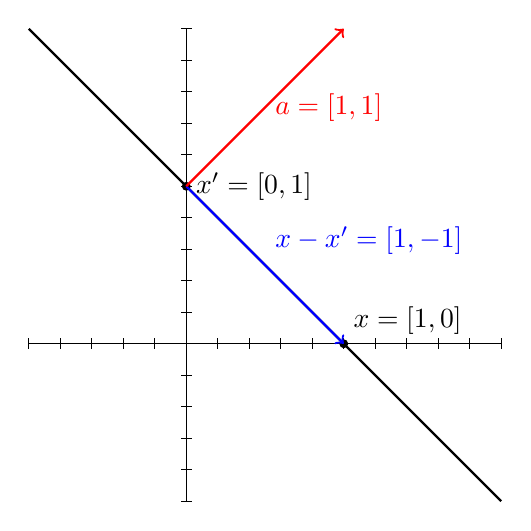
\begin{tikzpicture}[scale=2]
  %axis
  \draw (-1,0) -- coordinate (x axis mid) (2,0);
  \draw (0,-1) -- coordinate (y axis mid) (0,2);
  %ticks
  \foreach \x in {-1,-0.8,...,2}
    \draw (\x,1pt) -- (\x,-1pt);
  \foreach \y in {-1,-0.8,...,2}
  \draw (1pt,\y) -- (-1pt,\y);


  \draw[thick] (-1,2) -- (2,-1); 

  \fill (1,0) circle (.8pt) node [anchor=south west] {$x=[1,0]$};
  \fill (0,1) circle (.8pt) node [anchor=west] {$x'=[0,1]$};

  \draw[thick,->,blue] (0,1) -- node [anchor = south west] {$x-x'=[1,-1]$}  (1,0);
       
  \draw[thick,->,red] (0,1) -- node [anchor=west] {$a=[1,1]$} (1,2);

\end{tikzpicture}

\end{center}

\end{minipage}\hspace*{1cm}\begin{minipage}[t]{\textwidth-7cm}
  \vspace{0pt}
  Recall that in an $n$-dimensional space, a hyperplane $\cal H$ is a set of points \bm{x} satisfying
  an inequality $a_1x_1+\cdots+a_mx_m=1$ (the number one on the right hand side is almost without loss of
  generality: any hyperplane that does not contain the point  $[0,\ldots,0]$ can be normalized to this form).
  If we use the notation  $\pair{\cdot}{\cdot}$ for the scalar product, $\cal H$ is defined by 
   $\pair{\bm{x}}{\bm{a}}=1$. The points for which  $\pair{\bm{x}}{\bm{a}}<1$ are below the hyperplane,
   and points $\pair{\bm{x}}{\bm{a}}>1$ are above it. The vector \bm{a} is called a {\em normal } vector
   of $\cal H$ and for any two points \bm{x}, \bm{x'} from $\cal H$ it holds 
$$\pair{\bm{x}-\bm{x'}}{\bm{a}}=\sum_{i=1}^m(x_i-x'_i)a_i=\pair{\bm{x}}{\bm{a}}-\pair{\bm{x'}}{\bm{a}}=0.$$

\noindent
In two dimensions the hyperplane is a line; the one on the figure on the left is given by the equation
$x_1+x_2=1$.

\end{minipage}

\vskip 2mm
\noindent
Our discussion about convex hull concludes with the following observation that is completely obvious for two and 
three dimensions:

\begin{lema}
  \label{lm:KO:2}
  Consider points  $\bm{x},\bm{a_1},\ldots,\bm{a_n}$ in an $m$-dimensional space. 
  Let $K$ be the convex hull of 
  $\bm{a_1},\ldots,\bm{a_n}$. The it holds:
  \begin{itemize}
    \item 
      If \bm{x} is inside (i.e. $K$ contains \bm{x} with some small neighborhood) $K$, 
      then there is no hyperplane $\cal H$ 
      containing \bm{x} such that all points from $K$ are on one side
      (above or below) of $\cal H$.
    \item 
      If $\bm{x} \not\in K$,
      then there exists a hyperplane $\cal H$
      containing \bm{x} such that all points from $K$ are on one side
      (above or below) of $\cal H$.
  \end{itemize}
\end{lema}

\begin{dokaz}
  The first part is easy: let \bm{x} be inside $K$, and suppose there exists a hyperplane $\cal H$ such that
  all points from $K$ are one one side of $\cal H$. Since $\cal H$ contains \bm{x},
  there are two points in any close neighborhood of \bm{x} that lie on different sides of $\cal H$. 
  But \bm{x} is inside $K$, so there is some small neighborhood of \bm{x} contained in $K$.

\noindent
Now let us show the second part.
Consider a fixed point \bm{x}, and for all points $\bm{y}\in K$ consider the Euclidean distance 
$f(\bm{y}):=||\bm{y}-\bm{x}||$. Since $K$ is a compact set, and $f$ is a continuous function with positive codomain,
there is a point  $\bm{z}\in K$ where $f$ reaches minimum. Denote
  \begin{align*}
    \bm{t}&=\bm{x}-\bm{z} & \kappa&= \pair{\bm{t}}{\bm{x}}
  \end{align*}

\begin{minipage}[t]{4.5cm}
  \vspace{0pt}
  \begin{myfig}{\textwidth}{svg/CHa}
  \end{myfig}
\end{minipage}\hspace*{1cm}\begin{minipage}[t]{\textwidth-7cm}
  \vspace{0pt}
  Let$\cal H$ be the hyperplane consisting of points  \bm{y} for which $\pair{\bm{t}}{\bm{y}}=\kappa$.
  Clearly $\bm{x}\in{\cal H}$. It holds
  $$0\le\sum_{i=1}^m(x_i-z_i)^2=%\sum_{i=1}^mx_i^2-2x_iz_i+z_i^2=
  \bpair{x}{x}-2\bpair{x}{z}-\bpair{z}{z}$$
  and so
  \begin{align*}&\bpair{t}{z}=\pair{\bm{x}-\bm{z}}{\bm{z}}=\bpair{x}{z}-\bpair{z}{z}\le\\
                &\le\bpair{x}{x}-\bpair{x}{z}=\pair{\bm{x}-\bm{z}}{\bm{x}}=\bpair{t}{x}=\kappa
  \end{align*}
  \noindent
  Now it suffices to show that for all points $\bm{y}\in K$ it holds $\bpair{t}{y}\le\kappa$, and so
  they are on the same side of $\cal H$ as \bm{z}.
\end{minipage}

\noindent
Hence, let us consider $\bm{z}\in K$. 
Since \bm{z} minimizes the distance from  \bm{x}, and $K$ is a convex body, for all  $0\le\lambda\le1$ it holds
$||\bm{z}-\bm{x}||^2\le||(1-\lambda)\bm{z}+\lambda\bm{y}-\bm{x}||^2=
||(1-\lambda)(\bm{z}-\bm{x})+\lambda(\bm{y}-\bm{x})||^2$,
and from that after straightforward calculation
$0\le\lambda(\lambda-2)||\bm{z}-\bm{x}||^2+2\lambda(1-\lambda)\pair{\bm{z}-\bm{x}}{\bm{y}-\bm{x}}
+\lambda^2||\bm{y}-\bm{x}||^2
$.
Since $\lambda\ge0$, we have
$0\le(\lambda-2)||\bm{z}-\bm{x}||^2+2(1-\lambda)\pair{\bm{z}-\bm{x}}{\bm{y}-\bm{x}}
+\lambda||\bm{y}-\bm{x}||^2
$
and from that for the limit case  $\lambda\mapsto0$
we get $0\le\pair{\bm{z}-\bm{x}}{\bm{y}-\bm{x}}-||\bm{z}-\bm{x}||^2
=\pair{\bm{z}-\bm{x}}{\bm{y}-\bm{x}}-\pair{\bm{z}-\bm{x}}{\bm{z}-\bm{x}}
=\pair{\bm{z}-\bm{x}}{\bm{y}}-\pair{\bm{z}-\bm{x}}{\bm{z}}=\bpair{t}{z}-\bpair{t}{y}
$.
That's why
$\bpair{t}{y}\le\bpair{t}{z}\le\kappa$, what we wanted to prove.
\end{dokaz}

\end{shaded}

\noindent
Now let us get back to our goal -- to show that the same value of the primal and dual program we obtained
was not a coincidence. Let us consider the following example: for given $n$ points
 $\bm{a}_1,\ldots,\bm{a}_n$ from the
$m$-dimensional space
$\R^m$ (i.e. the point $\bm{a}_i$ has coordinates  $(a_{i1},a_{i2},\ldots,a_{im})$), and a vector 
$\bm{c}$, the goal is to find a largest possible number $\alpha\in\R^+$ such that  the point 
$\alpha\bm{c}$ is contained in the convex hull $K$ of the points  $\bm{a}_1,\ldots,\bm{a}_n$. 

\begin{minipage}[t]{3.2cm}
  \vspace{0pt}
  \begin{myfig}{\textwidth}{svg/dualityCHa}
  \end{myfig}
\end{minipage}\hspace*{1cm}\begin{minipage}[t]{\textwidth-5cm}
  \vspace{0pt}
  \vskip 2ex
\noindent 
Let us suppose, for the ease of exposition, that there is some solution, i.e. that the ray
generated by the vector $c$ hits $K$. From the convexity it follows that the intersection of $K$ and a line
is a line segment. The optimal solution is thus the point $\alpha\bm{c}$ where the ray leaves $K$. Following
Lemma~\ref{lm:KO:1}, the points of the convex hull can be expressed as a convex combination of the points
 $\bm{a}_1,\ldots,\bm{a}_n$,
 i.e. our unknown point $\alpha\bm{c}$ must be of the form $z_1\bm{a}_1+\cdots+z_n\bm{a}_n$
for some  $z_1,\ldots,z_n\ge0$ where  $\sum_{i=1}^nz_i=1$. 
Denoting  $y_j=\frac{z_j}{\alpha}$
for an arbitrary feasible point  $\alpha\bm{c}$ yields
\end{minipage}
\vspace*{-18mm}
  \begin{align*}
    y_j\ge&0 & \sum_{j=1}^ny_j=\frac{1}{\alpha} && \alpha\bm{c}=\alpha\sum_{j=1}^n\bm{a}_jy_j.
  \end{align*}
  To find a point that maximizes $\alpha$ means to find a point that minimizes $1/\alpha$.
  So we want to minimize the value  $\sum_{j=1}^ny_j$ over those $y_1,\ldots,y_n\ge 0$ for which
  $\sum_{j=1}^n\bm{a}_jy_j=\bm{c}$; just note that from given \bm{y}, \bm{z} and $\alpha$ can be reconstructed.
  Our task can be written as a linear program:
\begin{equation}
  \label{eq:dualCHa}
\begin{array}{rrrrrcl}
  {\rm minimize}     & y_1        & +\;y_2         & +\; \cdots  & +\;y_n   \\
  {\rm subject\ to} & a_{1,1}y_1 & +\;a_{2,1}y_2   & +\; \cdots  & +\;a_{n,1}y_n  & = & c_1 \\
            %              & a_{1,2}y_1 & +\;a_{2,2}y_2   & +\; \cdots  & +\;a_{n,2}y_n  & = & c_2 \\
                          &   \vdots   &   \vdots       &   \ddots   &  \vdots      &  \vdots & \vdots\\ 
                          & a_{1,m}y_1 & +\; a_{2,m}y_2   & +\; \cdots  & +\;a_{n,m}y_n  & = & c_m \\
                          &\multicolumn{4}{r}{y_1,\ldots,y_n}&\ge&0
\end{array}
\end{equation}

\noindent
or shorter
$$\text{(P)}\;\; \min_{\bm{y}\in\R^n}\left\{ \bm{1}\tr\bm{y} \mid A\tr\bm{y}=\bm{c},\;\bm{y}\ge\bm{0}\right\}, $$
where $A$ is an $n\times n$ matrix with rows formed by the coordinates of points  $\bm{a}_1,\ldots,\bm{a}_n$.
We apply our dualization recipe to the program (\ref{eq:dualCHa}) yielding a dual program

\noindent
\begin{minipage}[t]{4cm}
  \vspace{0pt}
  \begin{myfig}{\textwidth}{svg/dualityCHb}
  \end{myfig}
\end{minipage}\hspace*{1cm}\begin{minipage}[t]{\textwidth-5cm}
  \vspace{0pt}

\begin{equation}
  \label{eq:dualCHb}
  \text{(D)}\;\;  \max_{\bm{x}\in\R^m}\left\{ \bm{c}\tr\bm{x} \mid A\bm{x}\le\bm{1}\right\}
\end{equation}

\noindent
How can we interpret the solution of program  (\ref{eq:dualCHb})? Consider an arbitrary feasible solution
\bm{x}, and let ${\cal H}_{\bm{x}}$ be the hyperplane defined by points  \bm{y} for which  $\bpair{y}{x}=1$.
The constraints of program  (\ref{eq:dualCHb}) tell us that for any point  $\bm{a_i}$ it holds
$\bpair{a_i}{x}\le1$, and due to convexity the whole convex hull $K$ is below $\cal H$. Next, if we denote
$\alpha=\frac{1}{\bm{c}\tr\bm{x}}$, $\alpha\bm{c}$ is a point of the hyperplane ${\cal H}_{\bm{x}}$,
since $\pair{\alpha\bm{c}}{\bm{x}}=1$. Hence each feasible solution of (\ref{eq:dualCHb})
corresponds to a point $\alpha\bm{c}$ on a ray given by the vector \bm{c} that (following Lemma~\ref{lm:KO:2})
is not contained in $K$. Moreover, it is obvious that the optimum solution is non-negative, so we can without loss of
generality assume  $\bpair{x}{c}=||\bm{x}||\cdot||\bm{c}||\cos\varphi\ge0$, where $\varphi$
is the angle between the vectors \bm{x} and \bm{c}. Hence we are interested only in the feasible
solutions that correspond to the points $\alpha\bm{c}$ on the ray generated bu \bm{c} after it leaves $K$.
\end{minipage}

\vspace*{-4ex}
\noindent
The same holds also in the opposite direction: Take an arbitrary point $\alpha\bm{c}$ from the ray generated by \bm{c}
after it leaves $K$. Lemma~\ref{lm:KO:2}
asserts the existence of a hyperplane $\cal H$ such that all the points from $K$ are below $\cal H$. Let $\cal H$
consists of points \bm{y} for which $\bpair{x}{y}=1$ for some vector \bm{x}, then it holds
$A\bm{x}\le1$.
At the same time, since $\cal H$ contains $\alpha\bm{c}$, it holds $\pair{\bm{x}}{\alpha\bm{c}}=1=\alpha\bpair{x}{c}$,
and so $\alpha=\frac{1}{\bm{c}\tr\bm{x}}$.
For the maximum value $\bm{c}\tr\bm{x}$ the corresponding $\alpha$ is minimal, so the program
 (\ref{eq:dualCHb})
 actually asks to find a minimum $\alpha$ such that the point $\alpha\bm{c}$ is after $K$ on the ray generated by 
\bm{c}. This is, however, obviously the point where the ray leaves $K$, and so the programs 
(\ref{eq:dualCHa}) and (\ref{eq:dualCHb}) have the same optimal solution.
We proved the statement

\begin{lema}
  \label{lm:strongdualityprep}
  If the primal program $\min_{\bm{y}\in\R^n}\left\{ \bm{1}\tr\bm{y} \mid A\tr\bm{y}=\bm{c},\;\bm{y}\ge\bm{0}\right\}$
  has feasible solution, then also the dual program
$\max_{\bm{x}\in\R^m}\left\{ \bm{c}\tr\bm{x} \mid A\bm{x}\le\bm{1}\right\}$
has feasible solution, and the values of the optima in both programs are equal.
\end{lema}

\noindent
If we managed to generalize the Lemma~\ref{lm:strongdualityprep}
to the programs of the form
$\min_{\bm{y}\in\R^n}\left\{ \bm{b}\tr\bm{y} \mid A\tr\bm{y}=\bm{c},\;\bm{y}\ge\bm{0}\right\}$
for an arbitrary vector  \bm{b},
we would be happy, since any linear program can be expressed in that form. 
So, let us consider a linear program
\begin{equation}
  \label{eq:dualgenP}
  \text{(P)}\;\; \min_{\bm{y}\in\R^n}\left\{ \bm{b}\tr\bm{y} \mid A\tr\bm{y}=\bm{c},\;\bm{y}\ge\bm{0}\right\}
\end{equation}
and the corresponding dual program
\begin{equation}
  \label{eq:dualgenD}
  \text{(D)}\;\;\max_{\bm{x}\in\R^m}\left\{ \bm{c}\tr\bm{x} \mid A\bm{x}\le\bm{b}\right\}\hspace*{10ex}
\end{equation}
\noindent
First, let us consider all vectors \bm{b} with all entries $b_i>0$. Denote
\begin{align}
  \label{eq:dualgenNote1}
  \bm{a}_i'=&\frac{1}{b_i}\bm{a}_i & y_j'=&b_jy_j 
\end{align}

\noindent
It holds $\bm{b}\tr\bm{y}=\sum_{j=1}^nb_jy_j=\bm{1}\tr\bm{y}'$ and for each $i\in\{1,\ldots,m\}$ we have
$\sum_{j=1}^ma_{ji}y_j=\sum_{j=1}^ma'_{ji}b_i\frac{y_j'}{b_j}$. Since  $b_j>0$,  the program (\ref{eq:dualgenP})
is equivalent\footnote{in the sense that to every feasible solution of the program (\ref{eq:dualgenP}) 
there is some corresponding feasible solution of (\ref{eq:dualgen3}) with the same value, and vice versa} with
the program
\begin{equation}
  \label{eq:dualgen3}
  \min_{\bm{y'}\in\R^n}\left\{ \bm{1}\tr\bm{y'} \mid A'\bm{y'}=\bm{c},\;\bm{y'}\ge\bm{0}\right\} 
\end{equation}
Where the columns of the matrix $A'$ are the vectors $\bm{a}_i'$.
Following Lemma~\ref{lm:strongdualityprep}, if the program (\ref{eq:dualgen3}) has a feasible solution,
its optimum is the same as the optimum of the program
\begin{equation}
  \label{eq:dualgen4}
  \max_{\bm{x'}\in\R^m}\left\{ \bm{c}\tr\bm{x'}\mid {A'}\tr\bm{x'}\le\bm{1}\right\}
 \end{equation}
 The constraints of the program (\ref{eq:dualgen4} are of the form $\sum_{j=1}^ma_{ji}'x'_j\le1$
 and so by exploiting the notation  (\ref{eq:dualgenNote1}) we get that programs
 (\ref{eq:dualgen4}) and (\ref{eq:dualgenD}) are equivalent, so if (\ref{eq:dualgenP})
 has a feasible solution,  (\ref{eq:dualgenD}) has a feasible solution, too, and values of the optima
 are the same.


\begin{prob}
  Modify the previous approach so that it works also for $b_i\ge0$.
\end{prob}

\noindent
Now let \bm{b} have arbitrary values $b_i\in\R$, and  let $\bm{\tilde{x}}$ be a fesible solution of 
(\ref{eq:dualgenD}). Denote
\begin{align}
  \label{eq:dualgen5}
  \bm{x'}&=\bm{x}-\bm{\tilde{x}} & b_i'&=b_i-\bm{a}_i\tr\bm{\tilde{x}}
\end{align}

\noindent
How will the programs (\ref{eq:dualgenP}) and (\ref{eq:dualgenD}) look like in this notation?
For any feasible solutions \bm{x}, \bm{y} we have
$$
\begin{array}{ll}
  \bm{c}\tr\bm{x} &= \bm{c}\tr\bm{x'} + \bm{c}\tr\bm{\tilde{x}}\\
  \bm{b}\tr\bm{y} &= \sum_{i=1}^nb_iy_i = \sum_{i=1}^nb'_iy_i+\sum_{i=1}^ny_i(\bm{a}_i\tr\bm{\tilde{x}})=
  \bm{b'}\tr\bm{y}+\sum_{i=1}^ny_i\sum_{j=1}^ma_{i,j}\tilde{x}_j =\\
  &= \bm{b'}\tr\bm{y}+ \sum_{j=1}^m\tilde{x}_j(\sum_{i=1}^ny_ia_{i,j}) =
  \bm{b'}\tr\bm{y}+\bm{c}\tr\bm{\tilde{x}}
\end{array}
$$
where the last equality follows from $A\tr\bm{y}=\bm{c}$.
Since $\bm{c}\tr\bm{\tilde{x}}$ is constant, programs  (\ref{eq:dualgenP}) and (\ref{eq:dualgenD})
can be equivalently written  
\begin{align*}
  (\text{P}')\;\; \min_{\bm{y}\in\R^n}\left\{ \bm{b'}\tr\bm{y} \mid A\tr\bm{y}=\bm{c},\;\bm{y}\ge\bm{0}\right\}
  &&
 (\text{D}')\;\; \max_{\bm{x'}\in\R^m}\left\{ \bm{c}\tr\bm{x'} \mid A\bm{x'}\le\bm{b'}\right\}
\end{align*}

\noindent
Moreover, from the feasibility of $\bm{\tilde{x}}$ for (\ref{eq:dualgenD} it follows that $\bm{b'}\ge\bm{0}$,
and so the previous case applies.


\noindent
Hence, we have sketched\footnote{For a complete proof some more special cases have to be covered, 
a boring work that we gladly leave up to the enthusiastic reader.} the proof of a fundamental theorem
in the theory of linear programming:

\begin{framed}
  \begin{veta}[Strong duality theorem]
    \label{thm:strongduality}
    For a pair of linear programs
    \begin{align*}
      \text{(P)}\;\; \min_{\bm{y}\in\R^n}\left\{ \bm{b}\tr\bm{y} \mid A\tr\bm{y}=\bm{c},\;\bm{y}\ge\bm{0}\right\}
      &&
      \text{(D)}\;\;\max_{\bm{x}\in\R^m}\left\{ \bm{c}\tr\bm{x} \mid A\bm{x}\le\bm{b}\right\}\hspace*{10ex}
    \end{align*}
    exactly on of the following cases holds:
    \begin{enumerate}
      \item neither (P) nor (D) has any feasible solutions
      \item (P) is unbounded, and (D) has no feasible solutions
      \item (D) is unbounded, and (P) has no feasible solutions
      \item both (P) and (D) have feasible solutions, and the optimum values of (P) and (D) are equal.
    \end{enumerate}
  \end{veta}
\end{framed}

 
\newpage
\section{\maxflow--\mincut in the view of LP duality}

\noindent 
The LP duality, introduced in the previous section, often helps to better (or at least differently)
understand min-max characterizations of computational problems. In this part we employ the duality 
theory to give an alternative proof of the known fact that the size of the maximum $s-t$ flow equals to 
the capacity of the minimum $s-t$ cut. Since we suppose that the reader is already familiar with the 
\maxflow and \mincut problems, we abstain from motivational examples, and just recall the definitions.

\noindent
Given is an (undirected) graph $G=(V,E)$ with non-negative edge weights, i.e.
a mapping $c:E\mapsto\R^+$; instead of  $c(\{u,v\})$ we shall use a shorthand notation
$c_{uv}=c_{vu}$. In the graph, there are two distinguished vertices $a$ and $t$,
The \maxflow problem aims to maximize the flow from $s$ to $t$, where a flow is a mapping
$f:V^2\mapsto\R^+$, such that $f(u,v)$ represents the amount of a liquid that flows
from $u$ to $v$ in an unit time. The flow must hence satisfy the following properties:
\begin{enumerate}
  \item if $f(u,v)\not=0$ then  $(u,v)\in E$, i.e. the flow can be only along the edges of the graph
  \item $f(u,v)=-f(v,u)$, i.e. the sign gives the direction of the flow
  \item for each $v\not\in\{s,t\}$ it holds $\sum\limits_{u\in V}f(u,v)=0$, 
  known as a flow conservation law
  \item $|f(u,v)|\le c_{uv}$, i.e. the flow is bounded by the capacity of the edge
\end{enumerate}
\noindent
The size of the flow is  $\sum_{v\in V}f(s,v)$. 
A cut in $G$ is a set of edges in $G$ whose removal disconnects $s$, and $t$ (i.e. they are in different
connected components of the resulting graph). The \mincut problems asks to find a cut with minimal capacity.
The following figure depicts a graph with a minimum cut (left), and a maximum flow (right; the dark edges 
are those whose capacity is fully used by the flow) with value 24.


\begin{myfig}{\textwidth}{svg/flowcutNew}
\end{myfig}


\noindent
The \maxflow problem has a number of  natural formulations as a linear program. For reasons we hope
to become apparent by the end of this section we choose the following one: for each edge $(u,v)\in E$ 
we introduce two non-negative variables $x_{uv}$ and $x_{vu}$ that denote the amount of flow
along the edge $(u,v)$ (note that, by doing this, we allow to have a non-negative amount of flow $x_{uv}$ from
$u$ to $v$, and at the same time, some non-negative amount of flow $x_{vu}$ from $v$ to $u$; however,
it is easy to verify that simply subtracting the two values maintains the feasibility and value of a solution,
and makes it compatible with our definition of flow).  Next, we introduce a variable $f$ that will
denote the amount of the whole flow (and the goal will be to maximize $f$):
$f=\sum\limits_{u:(s,u)\in E}x_{su}-\sum\limits_{u:(s,u)\in E}x_{us}$. 
Flow conservation law, and the capacity constraints can easily be expressed as linear inequalities, yielding
the following program:

\begin{equation}
  \label{eq:flow:1}
  \begin{array}{rrcll}
      {\rm maximize}     & \multicolumn{1}{r}{f}\\[8mm]
    {\rm subject\ to} & \sum\limits_{u:(s,u)\in E} x_{su} - \sum\limits_{u:(s,u)\in E} x_{us} - f  &=&0&  \\[6mm]
                            & \sum\limits_{u:(t,u)\in E} x_{ut} - \sum\limits_{u:(s,u)\in E} x_{tu} + f  &=&0&  \\[6mm]
                            & \sum\limits_{u:(u,v)\in E} x_{vu} - \sum\limits_{u:(u,v)\in E} x_{uv} &=&0&\;\;\;
    \forall v\in V - \{s,t\}\\[6mm]
    & x_{uv}&\le& c_{uv}&  \;\;\;\forall (u,v)\in E\\[1mm]
    & x_{vu}&\le& c_{uv}&  \;\;\;\forall (u,v)\in E\\[1mm]
                            & x_{uv}&\ge& 0 &  \;\;\;\forall (u,v)\in E\\
  \end{array}
\end{equation}  

\noindent
The first two constraints define the size of the flow $f$ as the net amount that leaves $s$, or enters $t$,
respectively. All remaining vertices (the next set of constraints) obey the flow conservation law. 

\noindent
Now let us apply our dualization recipe, and look at the dual minimization program to the program (\ref{eq:flow:1})
Every constraint in the primal program gives rise to a variable in the dual program, In the program  (\ref{eq:flow:1})
there are two types of constraints: the constraints of the form $\cdots = 0$ for each vertex, and
constraints  $x_{uv}\le c_{uv}$. Introduce a dual variable  $y_v\in\R$ for each vertex $v\in V$
($y_s$ corresponds to the first constraint, $y_t$ to the second one, and the rest to the remaining vertices),
and a pair of non-negative variables $z_{uv}$ a $z_{vu}$ for each edge $(u,e)\in E$. The $i$-th dual variable
is a multiplier of the $i$-th constraint in the linear combination with the requirement that sum of the left-hand
sides is component-wise bigger than the maximized utility function. The sum of the right-hand sides is in 
our case $\sum\limits_{(u,v)\in E}(z_{uv}+z_{vu})c_{uv}$.
The maximized function is zero in all components but $f$. The variable $f$ appears only in the first and 
second constraints of  (\ref{eq:flow:1}), hence we get in the dual a constraint $y_t-y_s=1$
(note that although in the optimum solution $f$ clearly is non-negative, we did not require the variable $f\ge0$).
Every variable $x_{uv}$ appears in three constraints: the constrain corresponding to vertex the $u$ with positive sign,
the constraint corresponding to the vertex $v$ with negative sign, and in the constraint $x_{uv}\le c_{uv}$. 
Summarizing, we get the following program:

\begin{equation}
  \label{eq:flow:2}
  \begin{array}{rrcll}
    {\rm minimize}     & \multicolumn{1}{r}{\sum\limits_{(u,v)\in E}(z_{uv}+z_{vu})\,c_{uv}}\\[8mm]
    {\rm subject\ to} & y_t - y_s  &=&1&  \\[3mm]
                            & y_v - y_u + z_{uv} &\ge&0&\;\;\;    \forall (u,v)\in E \\[3mm]
                            & y_u - y_v + z_{vu} &\ge&0&\;\;\;    \forall (u,v)\in E \\[3mm]
                            & z_{uv},z_{vu}&\ge& 0 &  \;\;\;\forall (u,v)\in E\\
  \end{array}
\end{equation}  

\noindent
From the strong duality theorem we know that programs (\ref{eq:flow:1}) and (\ref{eq:flow:2})
have the same value of the optimum. How can we interpret the  program  (\ref{eq:flow:2})?
Without loss of generality we can suppose that at least one of the pair of variables  $z_{uv},z_{vu}$
is zero: the only constraints concerning  $z_{uv}$ or $z_{vu}$ are the constraints
$z_{uv}\ge y_u-y_v$ and $z_{vu}\ge y_v-y_u$. Clearly, at least one of the values 
 $y_u-y_v$ and  $y_v-y_u$ is not positive, and so we can set at least one of them to zero in any feasible solution,
and not increase the value of the utility function. Hence, we can denote $\bar{z}_{uv}=\max\{z_{uv},z_{vu}\}$;
the constraints then ensure that $\bar{z}_{uv}\ge|y_u-y_v|$ and using the same arguments as before we can
suppose without loss of generality  $\bar{z}_{uv}=|y_u-y_v|$.
Now we can see the  solving of the program as placing the vertices of the graph on a line: the vertex $v$
is placed in the point $y_v$, where again without loss of generality we may assume that $s$ is placed in $0$, and
$t$ in $1$. The value  $\bar{z}_{uv}$ is the length of the edge $(u,v)$ in this placement of vertices.
Altogether, the optimal solution of the program  (\ref{eq:flow:2}) places the vertices of the graph on a line
segment of length 1 in such a way that $s$ and $t$ are on the endpoints, and the overall length 
of edges, weighted by their capacity, is minimized.

\begin{myfig}{0.9\textwidth}{svg/relaxcut}
  A graph with edge weights (left) and one of possible optimal solutions (right) of the program
  (\ref{eq:flow:2}):
  $\bar{z}_{su}=\bar{z}_{vw}=\frac{1}{6}$, $\bar{z}_{sv}=\bar{z}_{uw}=\frac{1}{3}$,
  $\bar{z}_{sw}=\bar{z}_{wt}=\frac{1}{2}$. The resulting value is
  $$\sum_{(u,v)\in E}c_{uv}\bar{z}_{uv}=\frac{1}{6}+\frac{1}{3}+2\frac{1}{2}+\frac{1}{3}+\frac{1}{6}+4\frac{1}{2}=4.$$
\end{myfig}

\noindent
Now let us rewrite the program  (\ref{eq:flow:2}) in normal form 
$\max\{-\bm{c}\tr\bm{\beta}\mid A\bm{\beta}=0,\;\bm{\beta}\ge0\}$.
Introduce a slackness variable $\hat{z}_{uv}\ge 0$ to each variable  $z_{uv}$, obtaining the
constraints of the form  \hbox{$y_v-y_u+z_{uv}-\hat{z}_{uv}=0$}.
If the vector  $\bm{\beta}$ contains the values ordered as  
$y_s,y_t,y_{v_1},\ldots,z_{uv},z_{vu},\ldots,\hat{z}_{uv}.\hat{z}_{vu},\ldots$, 
the matrix $A$ has the following structure:

\begin{myfig}{0.8\textwidth}{svg/cutlp}
\end{myfig}

\noindent
The following straightforward chores are left to the reader:


\begin{prob}
  Using Theorems \ref{thm:idTum} and \ref{thm:unimod} prove that the matrix $A$ is TUM.
\end{prob}


\noindent
Theorem~\ref{thm:tumInteger} implies that there exists an integral optimal solution of the 
program (\ref{eq:flow:2}). It means that all vertices have $y_v\in\{0,1\}$, i.e. they are placed in one of 
the endpoints of the line, and each edge has length 0 or 1. That means that every $s-t$ path must contain at least
one edge with length 1, which implies that the removal of edges with length 1 disconnects $s$ and $t$.
So we can say

\begin{veta}[\maxflow-\mincut theorem]
  The size of the maximal flow is equal to the capacity of the minimal cut.
\end{veta}
\begin{dokaz}
  The size of the maximal flow is the optimum value of the program (\ref{eq:flow:1}), which is the same
  as the optimum of the program  (\ref{eq:flow:2}). There exists an integral optimum of (\ref{eq:flow:2})
  and at the same time there is a bijection between $s-t$ cuts and integral solutions of  (\ref{eq:flow:2}).
\end{dokaz}

\noindent
It is quite possible that the reader is familiar with a proof that is significantly simpler, and does not involve
the linear programming. The reason why we present this argument (apart from the fact that we want to 
give a more concrete  example of the LP duality) is that the \maxflow-\mincut pair is seen as a special case
of a general class of problems; at the same time, it sheds a new light into the question why a similar result 
does not hold for seemingly similar problems (e.g. we would have more sources and sinks, and the goal would be
to maximize the flow of several commodities in common networks of pipes, we would get a problem that is dual to the
relaxed version of the \minmulticut from Definition~\ref{dfn:multicut}, however, a similar result does not hold)
via the unimodularity of the corresponding matrices.
 
\section{The primal-dual method}

\noindent
We hope to have persuaded the reader that duality is an interesting property of linear programs. 
Now it is time to show that it is also a useful one. Let us consider the primal-dual pair of
linear programs

\begin{eqnarray*}
  (P):&\min\limits_{\bm{x}\in\R^n}\{\bm{c}\tr\bm{x}\mid A\bm{x}\ge\bm{b}, \bm{x}\ge 0\}\\
  (D):&\max\limits_{\bm{y}\in\R^m}\{\bm{b}\tr\bm{y}\mid A\tr\bm{y}\le\bm{c}, \bm{y}\ge 0\}
\end{eqnarray*}

\noindent
From the strong duality theorem we know that they have the same value of the optimum, i.e. there
exist vectors  $\bm{x^\star}\ge0$
and $\bm{y^\star}\ge0$, such that $A\bm{x^\star}\ge\bm{b}$, $A\tr\bm{y^\star}\le\bm{c}$
and $\bm{c}\tr\bm{x^\star}=\bm{b}\tr\bm{y^\star}$.
Recall the inequalities from the proof of Theorem\ref{thm:weakduality} that hold for
all pairs of feasible solutions of a primal-dual pair, and so in particular for $\bm{x^\star}$, $\bm{y^\star}$:

\begin{equation}
  \label{eq:proofSlack}
  \bm{c}\tr\bm{x^\star}\stackrel{(\clubsuit)}{\ge}\left(A\tr\bm{y^\star}\right)\tr\bm{x^\star}
=\bm{y^\star}\tr A\bm{x^\star}\stackrel{(\diamondsuit)}{\ge}\bm{y^\star}\tr\bm{b}
\end{equation}

\noindent
Since $\bm{c}\tr\bm{x^\star}=\bm{b}\tr\bm{y^\star}$, both $(\clubsuit)$ and $(\diamondsuit)$ 
must be equal. Let us have a look at the  $(\clubsuit)$, and expand the scalar product of vectors into a sum:

\begin{equation}
  \label{eq:kompl:1}
  \sum_{j=1}^n c_jx^\star_j=\sum_{j=1}^n\left[A\tr\bm{y^\star}\right]_jx^\star_j,
\end{equation}

\noindent
where the symbol $[\cdot]_j$ denotes the  $j$-th coordinate of a vector. 
From the feasibility of the dual solution we know that
$\bm{c}\ge A\tr\bm{y^\star}$; 
the inequality of the vectors holds in every coordinate, so for each $j$ it is
$c_j\ge\left[A\tr\bm{y^\star}\right]_j$.
For each $j$ there is $x^\star_j\ge0$, and so also  $c_jx^\star_j\ge\left[A\tr\bm{y^\star}\right]_jx^\star_j$,
which implies that in order the equality (\ref{eq:kompl:1}) to hold, the equality must hold separately in every 
coordinate.


\noindent
The same reasoning goes for the inequality  $(\diamondsuit)$, yielding the following characterization
of the optimum solutions:

\begin{framed}
\begin{veta}[slackness conditions]
  \label{thm:slackness}
Let \bm{x}, \bm{y} be feasible solutions of the primal and dual programs, respectively.
Then \bm{x}, \bm{y} correspond to the common optimal solution if and only if the following 
conditions hold:

\begin{itemize}
\item primal slackness conditions:
$$\forall\;1\le j\le n:\;{\rm\ either\ }\; x_j=0\; {\rm\ or\ }\sum_{i=1}^ma_{ij}y_i=c_j$$
\item dual slackness conditions:
$$\forall\;1\le i\le m:\;{\rm\ either\ }\; y_i=0\; {\rm\ or\ }\sum_{j=1}^na_{ij}x_j=b_i$$
\end{itemize}
\end{veta}
\end{framed}

\subsection*{Edmonds' algorithm for \minfactor}

\noindent
When we spoke about the simplex method of solving linear programs, we argued that it is an efficient, albeit 
not polynomial-time, algorithm. Also, we mentioned that there exist polynomial methods for solving LP. The
truth is that, polynomial or not, solving LP can be quite expensive, especially if the program is large. 
The slackness conditions present a tool to significantly reduce the complexity of LP-based algorithms:
since we have an equivalent characterization of the optimal solution, we don't have to solve the LP. 
Instead, if we construct, using an arbitrary algorithm, solutions of the primal and dual programs that
satisfy the slackness conditions, we know that we have optimum solution. The usual approach in the
primal-dual method is to maintain a pair of solutions of the primal-dual pair of programs, such that
we start with a good (but not feasible) primal, and a feasible (but far from optimum) dual solutions.
In a sequence of iterations, we improve the value of the dual solution while maintaining feasibility, 
and at the same time adjust the primal
solution so that it is ''closer'' to being feasible.  In the end, we have a feasible primal-dual pair, 
with hopefully the same (optimal) value. We shall illustrate this approach on an example.
Recall the problem \maxWBmatching:

{
  \renewcommand{\thedummy}{\ref{dfn:maxWBmatching}}
  \begin{dfn}
    Given a bipartite graph with edges labeled by non-negative weights, the\\ \maxWBmatching
    problem asks to select a set of edges with maximal overall weight in such a way that no
    two selected edges share a common vertex.
  \end{dfn}
}


In section \ref{sec-ilp} we formulated the problem as an ILP:

\begin{equation*}
\begin{array}{rrcll}
  {\rm maximize}     & \multicolumn{1}{l}{\sum\limits_{e\in E}\omega_ex_e}\\[3ex]
  {\rm subject\ to} & \sum\limits_{e\in E\atop e=(v,w)}x_e&\le&1& \;\;\;\forall v\in V\\
                          & x_e&\ge&0& \;\;\;\forall e\in E\\
                          & x_e&\in&\Z
\end{array}
\end{equation*}

\noindent
where $\bm{\omega}\in\R^n$ is the vector of edge-weights. We showed that the matrix of constraints is TUM,
and thus it is sufficient to solve the relaxed program, and we have the integrality of the optimum
solutions for free. Quite naturally, we can ask: What happens if the graph is not bipartite? The formulation
of the ILP is still valid (we haven't used the fact that the graph was bipartite), but it is not true
anymore that the optimum solution is always integral.

\begin{myfig}{0.8\textwidth}{svg/matchingLP}
  On the left there is a graph with its edge-weights where the maximum matching has value $21$:
  edges of weight 10 are only among vertices $\{p,q,r,s,t\}$, so in any solution there can be at most two of them.
  From the remaining two edges, any solution can contain only one. On the right there is a solution of
  the relaxed program with value $25$.
\end{myfig}

\noindent
Before we continue we reformulate our problem slightly. A matching that covers all vertices, i.e. the 
set of edges $E'\subseteq E$ such that every vertex is incident with exactly one edge from $E'$ will
be called a {\em perfect matching} or a {\em 1-factor}. Obviously, in order a graph could have a 1-factor, it
has to have even number of vertices. Instead of finding the heaviest matching, it is sufficient to be able
to find the heaviest 1-factor: we first adjust the input graph $G$ such that if it has odd number of vertices
we add a new isolated vertex, and then we connect all pairs of vertices that are not connected by an existing
edge, by new edges with weight 0. It is easy to check that matchings in $G$ correspond to 1-factors in $G'$,
and vice-versa. Next, if $\omega_{\max}$ is maximum weight of an edge in $G'$. If we replace the weights
of all edges from $\omega_e$ to $\omega_{\max}-\omega_e$, we get the following definition:

\begin{framed}
  \begin{dfn}
    \label{dfn:minFactor}
    Given is a complete graph $G=(V,E)$ with even number of vertices and non-negative edge weights
    $\omega_e\in\R^+$. The problem \minfactor is to find a 1-factor of $G$ that minimizes the
    sum of weights, i.e. with weight $\min_{E'}\sum_{e\in E'}\omega(e),$ where the minimum is taken
    over all 1-factors of $E'$ of $G$.
  \end{dfn}\end{framed}


\noindent
The reader who was patient enough to bear with us up to now can easily express \minfactor as an ILP:
for each edge $e\in E$ we introduce a variable $x_e\in\{0,1\}$ denoting whether $e$ is selected in the matching
or not. The selected set of edges is a 1-factor exactly if there is exactly one selected edge incident to
any vertex; this can be expressed in a straightforward way

\begin{equation}
  \label{eq:1f:ILP}
\begin{array}{rrcll}
  {\rm minimize}     & \multicolumn{1}{l}{\sum\limits_{e\in E}\omega_ex_e}\\[3ex]
  {\rm subject\ to} &  \sum\limits_{e\in E\atop e=(u,v)} x_e &=&1& \;\;\;\forall v\in V\\
                          & x_e&\in&\{0,1\}& \;\;\;\forall e\in E\\
\end{array}
\end{equation}

\noindent
If we relax this program by considering $x_e\ge0$ instead of  $x_e\in\{0,1\}$ (note that  $x_e\le1$
is implied by the minimization), the optimum is not necessarily integral. We shall now present the
primal-dual approach according to Edmonds \cite{Edmonds65}. Before that, however, we introduce one more
notation that simplifies the subsequent text:


\begin{dfn}[edge boundary of a set of vertices]
  \label{dfn:edgeboundary}
Given a  graph  $G=(V,E)$, and a set of vertices $S\subseteq V$, the edge boundary of the set $S$,
denoted $\partial(S)$, is the set of edges with one endpoint in $S$, and the other outside of $S$, 
i.e.
$$\partial(S):=\{e\in E\mid e=(u,v),\;u\in S,\;v\in V\setminus S\}$$
\end{dfn}

\noindent
How should we cope with the fact that the program  (\ref{eq:1f:ILP}) has no integral optimum? The main
idea is to augment the program with many additional constraints that have no impact on the ILP, but they
force the relaxed program to have integral optimum. Let \S be the family of all sets of vertices 
with odd size, containing at least three vertices, i.e.

$$\S:=\left\{ S\subseteq V\mid\; |S|>1,\;|S|\;{\rm\ odd\ }\right\}$$

\noindent
Every edge has two endpoints, so the vertices from any  $S\in\S$ cannot be paired among themselves, meaning
that in any 1-factor there must be at least one edge outgoing from $S$. We add these constraints explicitly 
to the relaxed program
(\ref{eq:1f:ILP}),
obtaining

\begin{equation}
  \label{eq:1f:P}
\begin{array}{rrcll}
  {\rm minimize}     & \multicolumn{1}{l}{\sum\limits_{e\in E}\omega_ex_e}\\[4ex]
  {\rm subject\ to} &  \sum\limits_{e\in\partial(\{v\})} x_e &=&1& \;\;\;\forall v\in V\\[4ex]
                          & \sum\limits_{e\in\partial(S)}x_e&\ge&1&\;\;\;\forall S\in\S\\[4ex]
                          & x_e&\ge&0& \;\;\;\forall e\in E\\
\end{array}
\end{equation}

\noindent
\ldots and {\em voilà!} We have a linear program with integral optimum solution. However, now we not only have to 
show that indeed the optimum solution of the program (\ref{eq:1f:P}) is integral, but we have to cope with a 
program that has exponentially many constraints. Neither of these problems is unsurmountable, as there are
methods that allow us to solve, under some assumptions that are satisfied in this case, in polynomial time
even linear programs with exponentially many (in fact, even with infinitely many) constraints. However, we 
have a more clever solution in mind: We avoid solving (\ref{eq:1f:P}) by using duality, and the integrality
proof comes for free. 

\noindent
Let us now use our dualization recipe and write down the dual program to  (\ref{eq:1f:P}).
It is a maximization program with a variable for each constraint of the original program. There are two
types of constraints in the original program: the ones concerning vertices and the ones concerning sets,
so let us introduce two sets of variables: $r_v\in R$ for $v\in V$
and $w_S\in\R^+$ for $S\in\S$.
Every primal variable $x_e$ contributes $x_e\omega_e$ to the utility function, and appears in two 
vertex-constraints (the ones for the endpoints of $e$) and in the set-constraints for the sets 
$S\in\S$ where $e\in\partial(S)$. We obtain the following program (note that $r_v$ may be also negative):

\begin{equation}
  \label{eq:1f:D}
\begin{array}{rrcll}
  {\rm maximize}     & \multicolumn{1}{l}{\sum\limits_{v\in V}r_v + \sum\limits_{S\in\S}w_S}\\[4ex]
  {\rm subject\ to} & 
        r_u + r_v + \sum\limits_{S\in\S\atop e\in\partial(S)} w_S &\le&\omega_e& \;\;\;\forall e=(u,v)\in E\\[4ex]
                          & w_S&\ge&0& \;\;\;\forall S\in\S\\
\end{array}
\end{equation}

\noindent
For the explanatory reasons, and also because in our pair of programs not all variables are non-negative,
let us recall the inequality  (\ref{eq:proofSlack}):

$$
\sum_{e\in E}x_e\omega_e
\stackrel{\clubsuit}{\ge}
\sum_{e\in E\atop e=(u,v)}x_e(r_u+r_v+\sum_{S\in\S\atop e\in\partial(S)}w_S)
\stackrel{\heartsuit}{=}
\sum_{v\in V}(r_v  \textcolor{blue}{\sum_{e\in\partial(\{v\})}x_e} )   + \sum_{S\in\S}w_S
\textcolor{red}{\left(\sum_{e\in\partial(S)}x_e\right)}
\stackrel{\diamondsuit}{\ge}
\sum_{v\in V}r_v+\sum_{S\in\S}w_S
$$


\noindent
The equality in $(\heartsuit)$ comes due to the fact that every vertex $v\in V$
contributes by $r_vx_e$ to all edges $e$ incident with $v$, and every set $S\in\S$ 
contributes by $w_sx_e$ to all edges from the edge boundary of $S$. The constraints of the program 
(\ref{eq:1f:P}) imply that the blue sum $\sum_{e\in\partial(\{v\})}x_e=1$ and 
the red sum $\sum_{e\in\partial(S)}x_e\ge1$; hence, the slackness conditions are of the form


$$\begin{array}{lrl}
  {\bf S1} (\clubsuit) \;\;&\forall e=(u,v)\in E:\;\;&x_e>0\Rightarrow r_u + r_v +
  \displaystyle\sum\limits_{S\in\S\atop e\in\partial(S)}w_S=\omega(e)\\[6ex]
  {\bf S2} (\diamondsuit)\;\;&\forall S\in\S:\;\; & w_S>0\Rightarrow \displaystyle\sum\limits_{e\in\partial(S)}x_e=1
\end{array}$$


\noindent
Now have a look at the program (\ref{eq:1f:D}) and try to find some intuitive interpretation. Imagine that there is a 
bubble around every vertex $v\in V$, and every set $S\in\S$, carrying a charge of $r_v$, and $w_S$, respectively.
Clearly, the sets $S\in\S$ may overlap, making the image of bubbles sort of weird, however, in the final algorithm
we end up using only selections of non-overlapping bubbles. The program (\ref{eq:1f:D}) aims at maximizing
the overall charge. The edge weights can be considered a capacity, and the constraints require that no edge $e$
is overcharged: the overall charge on all bubbles that $e$ crosses cannot be more than its capacity.
An edge $e$ for which  $ r_u + r_v + \sum_{S\in\S\atop e\in\partial(S)}w_S=\omega(e)$ will be called {\em full}.
The conditions  {\bf S1} and {\bf S2} can, together with the strong duality theorem, provide the following 
observation

\begin{lema}
  \label{lm:1f:opt}
  If we find a 1-factor $M$, and the assignment of the charge to the bubbles  \bm{r} and \bm{w} 
  in such a way that
  \begin{itemize}
    \item[{\bf (I1)}] no edge is overcharged,
    \item[{\bf (I2)}] all $w_S\ge 0$,
    \item[{\bf (I3)}] all edges from $M$ are full, and
    \item[{\bf (I4)}] from each non-zero bubble  $S\in\S$ there is exactly one outgoing edge from $M$,
\end{itemize}
  then we have an optimal solution of the primal-dual pair of programs (\ref{eq:1f:P}) and (\ref{eq:1f:D},
  with an integral value of \bm{x}, and thus a minimum 1-factor.
\end{lema}

\begin{dokaz}
  The conditions {\bf (I1)} and {\bf (I2)} guarantee the feasibility of the dual program  (\ref{eq:1f:D}).
  The fact that $M$ is a 1-factor guarantees the feasibility of the primal program  (\ref{eq:1f:P}).
  The conditions  {\bf (I3)} and {\bf (I4)} are, respective, the slackness conditions {\bf S1} and {\bf S2},
  so the statement is a corollary of Theorem~\ref{thm:slackness}.
\end{dokaz}

\noindent
From this moment on we can forget about the whole linear programming business, and concentrate on 
finding an algorithm that constructs the desired objects $M$, \bm{r}, and \bm{w}. As we already hinted,
since the whole vector \bm{w} is too big, we shall explicitly store only the non-zero entries; at the same
time, we shall be looking only for solutions where the sets with non-zero bubbles do not intersect each other. 
We are seeking the following structure:

\vbox{
\begin{myfig}{0.8\textwidth}{svg/edmondsOverview}
  The blue bubbles have all value $1/2$, the edges that are not drawn have weight $\infty$. The red edges form a 
  1-factor. No edge is overcharged, all red edges are full, and there is exactly one outgoing red edge from 
  each green bubble. Hence, we know that the red 1-factor is minimum.
\end{myfig}
}


\noindent
Of course, so far we have no guarantee that such a configuration always exists. However, if we prove it, and 
find an algorithm that constructs it, we can check the task as finished and celebrate.


\noindent
Let us begin with an informal description of the algorithm. During the whole computation, the 
conditions  {\bf (I1)}, {\bf (I2)} and {\bf (I3)} will be maintained as invariants. The algorithm starts with
an empty matching $M$ and all bubbles zero. Gradually, the charge of some bubbles will be increased, and 
some edges will be added to the matching so that, in the end, $M$ is 1-factor, and the condition  {\bf (I4)}
holds; then $M$ is the minimum 1-factor. In the first step the charge is put to all bubbles $r_v$ simultaneously
(in the rest of the description, we shall call these bubbles {\em blue}, whereas the bubbles
$w_S$ will be called {\em green}). The first step ends when no more charge can be put to blue bubbles, 
because some edge $e=(u,v)$ became full. The edge $e$ is then added to the matching $M$, and the bubbles
$r_u$ and $r_v$ won't be incremented in the next step: they will form a {\em dumbbell}. Ultimately, 
an edge $e$, whose one endpoint is a vertex that is already incident with an edge from $M$, becomes full.
This edge is full, meaning that the bubbles at its ends cannot be increased, however, it cannot be added to $M$.
We shall call it a  {\em blocking} edge, and the algorithm shall maintain a set of blocking edges $L$.



\begin{myfig}{0.6\textwidth}{svg/edmonds1-en}
\end{myfig}

\noindent
Apart from free bubbles and dumbbells, a new structure has just formed: a path of length 3 composed of 
a blocking edge from $L$, and a matching edge from $M$; paths containing alternating edges from $L$ and $M$
will be called {\em alternating paths}. If, in the next iteration, the charge of the {\em free } bubbles 
will be increased by $+\varepsilon$, the odd and even bubbles from the alternating paths will receive 
the change of $+\varepsilon$ and $-\varepsilon$, respectively, as to not overcharge any edge; recall that,
unlike the green bubbles, the blue bubbles can have negative charge. In the next iteration, edges connecting
to bubbles where the charge is being increase may become full, which gives rise to trees of the alternating paths
(called {\em Hungarian trees}). A welcomed case is if the newly filled edge creates an alternating path with odd 
number of vertices, in this case the matching can be increased by swapping the membership of $L$ and $M$ edges 
along the path, and instead of an alternating path we have a set of dumbbells.


\begin{myfig}{0.9\textwidth}{svg/edmonds2-en}
\end{myfig}

\vspace*{-5ex}
\noindent
What should we do, however, if an edge becomes full, that connects two bubbles in a single tree? This is
the moment when the time has come for the green bubbles to play their part, and to the hierarchic structures
of bubbles.

\vskip 2ex
\noindent
The basic data structure of the algorithm is a {\em flower}. Each flower has an outer bubble, and inside it
a distinguished vertex called {\em stem}. The most simple flower is a single vertex surrounded by a blue bubble.
More complex flowers are formed by induction: take an odd number of flowers $K_1,K_2,\ldots,K_{2r+1}$, $r\ge 1$ 
(i.e. at least three flowers) such that the stems of the flowers $K_{2i}$ and $K_{2i+1}$ for $i=1,\ldots,r$
are connected by an edge from $M$, and at the same time for each pair of flowers 
$A:=K_{2i-1}$ and $B:=K_{2i}$ for $i=1,\ldots,r$, and $A:=K_{2r+1}$ and $B:=K_1$, there exist vertices 
$u\in A$ and $v\in B$, such that the edge $(u,v)\in L$. Then the green bubble surrounding  $K_1,\ldots,K_{2r+1}$ 
created a new flower, whose stem is the stem of the flower $K_1$. Flowers that are not parts of another flower
are called {\em outer flowers}.

\begin{myfig}{0.7\textwidth}{svg/edmonds3}
  \centerline{Examples of flowers with stems denoted by a square. The red edges are from $M$, 
  the black ones are from $L$.}
\end{myfig}

\noindent
It is worth noting that a flower encapsulates a part of the graph that is ''almost done'': with the exception of the 
stem, all vertices of the flower are pairwise matched by edges from $M$. At the same time 
exactly one edge from $M$ leaves any bubble in flower that 
does not contain the stem; from the bubbles
that contain the stem, on the other hand, leaves no edge from $M$. The previous observation is crucial for
the understanding of the algorithm, and we recommend the reader to devise a detailed proof of it using induction.
If there is a full edge connecting stems of two flowers, we can add it to $M$, and obtain a dumbbell. If all
vertices of the graph are included in dumbbells, the algorithm is finished.


\noindent
\begin{minipage}[t]{0.45\textwidth}
  \vskip 0pt
\begin{myfig}{\textwidth}{svg/edmonds4}
  \centerline{ The {\em shift} operation on a Hungarian tree.}
\end{myfig}
\end{minipage}
\hfill
\begin{minipage}[t]{0.5\textwidth}
  \vskip 0pt

\noindent
Free flowers that do not form dumbbells are organized in Hungarian trees. The flower on level 0 is {\em root} 
of the tree, the stem of a flower on level $2h-1$ is connected by an edge from $M$ with the stem of a flower
of level $2h$. If $K$ is a flower on level $2h$, and $H$ is a child of $K$ in the tree, then there is
an edge from $L$ connecting some vertex from $K$ to some vertex from $H$. The intuition is as follows:
the root of the tree is a flower that we would like to include in a dumbbell, but in order to do so, we
need a full edge connecting its stem to the stem of some other flower. However, there is no such edge, and
we cannot add more charge to the outer bubble of the flower to make some edge full, because there are other
edges crossing the outer bubble that are already full: the blocking edges from $L$; these edges lead to 
the flowers that are the children of the root, and so on. 

\noindent
During its computation, the algorithm maintains a set
of Hungarian trees, and the rest of the graph is covered by dumbbells. The algorithm 
works in iterations: in one iteration it performs a {\em shift} operation on all trees. The operation
adds some $\varepsilon$ charge to the outer bubbles of all flowers on 
\end{minipage}

\noindent
even levels, and subtracts the
same value from the outer bubbles of flowers on odd levels. The value of $\varepsilon$ is chosen as the
biggest value that does not violate the conditions {\bf (I1)}, {\bf (I2)}. The conditions may 
be violated by several ways:

\noindent
{\bf (P1) The charge of a green bubble on odd level dropped to 0. }
Let $K$ be the flower whose outer bubble reached zero charge. By the definition of a flower, $K$
contains an odd number of flowers $K_1,\ldots,K_{2r+1}$, such that the stem of $K$ is in  $K_1$.
Since $K$ is on odd level in the tree, $K$ has one parent, and (exactly) one child connected
stem-to-stem by an edge from $M$. Let the edge from $L$ connecting $K$ to its parent is from some
vertex in the flower $K_t$, and without loss of generality, let $t$ be odd. Then the
path $K_1,K_2,\ldots,K_t$ contains an odd number of flowers and can replace $K$ in the tree.
The pairs of flowers $K_{t+1},K_{t+2}$ up to $K_{2r},K_{2r+1}$ form dumbbells. The full edges
between $K_t$ and  $K_{t+1}$, and $K_1$ and $K_{2r+1}$ can be removed from $L$, since in the 
new tree, each of them has one endpoint on an odd level, and the other one in a dumbbell, so in the
next iteration they will not be full anymore. 

\begin{myfig}{0.8\textwidth}{svg/edmonds5}
\end{myfig}

\vspace*{-4ex}
\noindent
{\bf (P2) An edge $e$ connecting a flower $K$ on an even level, and a dumbbell $H$, has become full.} 
Let the dumbbell $H$ consist of flowers $H_1$ and $H_2$, so that $e$ leads to some vertex in $H_1$. The
edge $e$ will be included in $L$, and $H$ will join the corresponding tree so that $K$ (on even level)
will have a child $H_1$ (on odd level), and $H_1$ will have a child $H_2$ (on even level).

\begin{myfig}{0.7\textwidth}{svg/edmonds6}
\end{myfig}

\vspace*{-4ex}
\noindent
{\bf (P3)  An edge $e$ connecting flowers $K$ and $H$ in one tree has become full.}
Clearly, both $K$ and $H$ are on even level. Let $W$ be the closest common ancestor of $K$ and $H$. Since $W$
has at least two children, it must be also on an even level. Let  $K,K_1,\ldots,K_{2k+1},W$ and
$H,H_1,\ldots,H_{2r+1},W$ be two paths in the tree. From the parity of their  lengths it follows that they
can be wrapped in a new outer bubble to obtain a flower $Z$ on even level, whose stem is the stem of $W$.
The children of $Z$ are all the children of included flowers, they remain on odd levels. 

\begin{myfig}{0.8\textwidth}{svg/edmonds7}
\end{myfig}

\vspace*{-4ex}
\noindent
{\bf (P4) An edge $e$ connecting flowers $K$ and $H$ in two different trees ${\cal T}_1$ and ${\cal T}_2$ 
has become full.}
This is actually the core of the algorithm where the matching $M$ is increased. It is done by finding 
an alternating path connecting the stem of the root of ${\cal T}_1$ with the stem of the root of 
${\cal T}_2$. Since an edge became full, both flowers $K$ and $H$ are on even levels in their respective trees,
meaning that there is a path $K,K_1,\ldots,K_{2r}$ in ${\cal T}_1$, and a path $H,H_1,\ldots,H_{2q}$ 
in the tree ${\cal T}_2$, where $K_{2r}$ and $H_{2q}$ are roots of the respective trees. 
Both paths are formed by the edges of the trees, which are also edges of the original graph $G$, and
edges belonging to $L$ and $M$ are alternating on them, such that an edge from $M$ connects 
stems of neighboring flowers. In order to augment this alternating path in the trees
to an alternating path in the graph $G$ we observe the following:

\begin{lema}
  \label{lm:1f:tmp1}
  Let $K$ be a flower with a stem  $u$, and let $v$ be an arbitrary vertex from $K$. Then there
  exists an alternating path in $G$ from $u$ to $v$ fully contained in $K$, and if this path is
  non-empty it starts with an edge from $L$ and ends with an edge from $M$.
\end{lema}


\begin{dokaz}
  We prove the lemma by induction on the depth of recursion of the flower. For a flower with a single
  vertex the statement holds trivially. Further, let $K$ be a flowers composed of sub-flowers
  $K_1,\ldots,K_{2r+1}$ such that the stem of $K$ is the stem of $K_1$. Without loss of generality
  let $v\in K_{2t-1}$ for some $t$ (if $v\in K_{2t}$ we just change the direction of the
  numbering of the sub-flowers). If $t=1$ we can use the induction hypothesis on the flower $K_1$.
  So let us assume $t>1$. From the definition of the flower we can infer the existence of an edge
  $(q,w)\in L$ such that $q\in K_1$ and $w\in K_2$. By induction, there is an alternating $u-q$ path in $K_1$
  that ends by an edge from $M$. At the same time there is an alternating path
  in $K_2$ from the stem to $w$ that ends by an edge from $M$. Joining these two paths together, we get
  an alternating path from $u$ to the stem of $K_2$ that ends by and edge from $L$, and so can be extended
  to the stem of $K_3$. Iterating this construction we obtain an alternating path to the stem of $K_{2t-1}$
  that can, again by the induction hypotheses, be extended to $v$. 
\end{dokaz}


\noindent
The construction from Lemma~\ref{lm:1f:tmp1} 
enables us to find an alternating path from the stem of $K_{2r}$ and the stem of $K_{2q}$. Along this path, 
we swap the membership of edges to $L$ and $M$, thus increasing the number of edges in $M$ by one. Subsequently,
the trees ${\cal T}_1$ and ${\cal T}_2$ can be dismantled: the flowers $K_{2i-1}$ and $K_{2i}$ (and, similarly,
$H_{2j-1}$ and $H_{2j}$) form after the swap a set of dumbbells. To see this it is sufficient to note that
the path from the proof of Lemma~\ref{lm:1f:tmp1} either does not cross a given flower, or crosses it 
exactly twice, once by an edge from $M$, and once by an edge from $L$. Hence, after the swap we keep the invariant
that every bubble is crossed by exactly one edge from $M$, and the stem of the tree is moved to the vertex $v$ 
specified by Lemma~\ref{lm:1f:tmp1}. Similarly, the flowers $K$ and $H$ form a dumbbell, and the 
remaining subtrees of both  ${\cal T}_1$ and ${\cal T}_2$ form dumbbells in a natural way.

\begin{myfig}{\textwidth}{svg/edmonds8}
\end{myfig}


\noindent
The final algorithm works in a cycle: while $M$ is not a 1-factor, one iteration finds the smallest
value $\varepsilon$ such that the shift by $\varepsilon$ violates some of the conditions  {\bf(I1)},  {\bf(I2)} 
from Lemma~\ref{lm:1f:opt}. According to what situation occured, one of the actions  {\bf(P1)},  {\bf(P2)}, {\bf(P3)} 
or {\bf(P4)} is executed, and a next iteration begins. The condition {\bf (I3)} remains true as an invariant.
When the algorithm terminates, $M$ is a 1-factor, and no flower can be a root of a tree (it would mean
its stem is not matched in $M$, so $M$ would not be a 1-factor); hence, all vertices are included in dumbbells,
and the condition {\bf (I4)} holds, too. Lemma~\ref{lm:1f:opt} then implies that when the algorithm terminates,
$M$ is a minimum 1-factor.

\noindent
The only thing to show now is that the algorithm indeed terminates, and if possible also that it terminates soon
enough. Our argument is based on the following observation:

\begin{lema}
  The described algorithm for the \minfactor problem performs at most $O(n^2)$ iterations on an $n$-vertex graph $G$.
\end{lema}
\begin{dokaz}
  The size of $M$ never decreases, and is increased by 1 in every execution of the action {\bf (P4)}.
  Hence, the algorithm may perform at most $O(n)$ times the action  {\bf (P4)}. In order to prove the statement
  it is sufficient to show that between two consecutive executions of the action {\bf (P4)} there are at most
  $O(n)$ iterations of the algorithm, performing actions  {\bf (P1)}, {\bf (P2)} and {\bf (P3)}.


\noindent
  The first thing to note is that at any point during the execution there are at most $O(n)$ bubbles
  overall (including the bubbles inside flowers). This is due to the fact that every flower contains at least three
  sub-flowers, and so if we call the {\em depth} of the flower the length of a maximum chain of included bubbles,
  then at any time the algorithm can maintain at most $n$ flowers of depth 0, $n/3$ flowers of depth 1, $n/3^2$
  flowers of depth 2, and so on, forming a geometric series.


\noindent
 Now let us consider the computation of the algorithm between two executions of the action  {\bf (P4)}.
 Another important observation is that the charge of an outer bubble of a flower on even level will never decrease:
 either it remains as an outer bubble of a flower of even level, or it becomes part of another flower
 of even level in action  {\bf(P3)}).  We shall call as {\em safe bubble} a bubble that was, at some point
 during the considered period of computation between two executions of  {\bf (P4)}, an outer bubble
 of a flower on even level. To finish the proof it is sufficient to show that actions  {\bf (P1)}, {\bf (P2)} and
 {\bf (P3)} increase the number of safe bubbles. <since the safe bubbles never disappear and there are linearly 
 many bubbles overall, we obtain that between two consecutive executions of  {\bf (P4)}, at most linearly many
 other iterations may occur. 


 \noindent
 The action  {\bf (P1)} destroys a bubble $B$ on odd level, and at least one bubble $B'$ from its inside
 appears on an even level. This bubble, however, was not safe before, since a safe bubble never becomes a part
 of a flower on odd level. The action  {\bf (P2)} adds a safe bubble from the dumbbell, and the action
 {\bf (P3)}  creates a new safe bubble.
\end{dokaz}


\noindent
A straightforward implementation of one iteration runs in time $O(nm)$, where $n$ is the number of vertices, and $m$
is the number of edges: for each edge, check all bubbles and check what largest $\varepsilon$ this edge still allows.
Select the edge with smallest bound, and perform the corresponding action. Hence, we can say:

\begin{veta}
  The \minfactor problem is solvable in time $O(n^3m)$.
\end{veta}

\noindent
For an insightful reader we may add that using a more clever data structures, the running time can be significantly
improved; it is, however, beyond the scope of this text.



%%%%%%%%%%%%%%%%%%%%%%%%%%%%%%%%%%%%%%%%%%%%%%%%%%%%%%%%%
\subsection*{Relaxed slackness conditions}


\noindent
In the previous part we introduced the primal-dual method based on the characterization of optimal solutions
by slackness conditions. For a  primal-dual pair of programs

\begin{eqnarray*}
  (P):&\min\limits_{\bm{x}\in\R^n}\{\bm{c}\tr\bm{x}\mid A\bm{x}\ge\bm{b}, \bm{x}\ge 0\}\\
  (D):&\max\limits_{\bm{y}\in\R^m}\{\bm{b}\tr\bm{y}\mid A\tr\bm{y}\le\bm{c}, \bm{y}\ge 0\}
\end{eqnarray*}

\noindent
the vectors $\bm{x}$ and $\bm{y}$ are optimal solutions of $(P)$ and $(D)$, respectively, if and only if

\begin{eqnarray*}
  \forall\;1\le j\le n:\;{\rm\ either\ }\; x_j=0\; {\rm\ or\ }\sum_{i=1}^ma_{ij}y_i=c_j\\
  \forall\;1\le i\le m:\;{\rm\ either\ }\; y_i=0\; {\rm\ or\ }\sum_{j=1}^na_{ij}x_j=b_i
\end{eqnarray*}

\noindent
Now we want to use this method to obtain an approximate solution of some \NP-hard optimization
problems. Can this characterization be of any help? Can we, for example, say that if we have a pair of
vectors \bm{x}, \bm{y} that violate the slackness conditions, but only a ``little bit'', then we can
obtain a solution that is ``almost'' optimal? Indeed, we can modify the Theorem~\ref{thm:slackness}
as follows:


\begin{framed}
\begin{veta}
  \label{thm:slacknessrelax}
   Let \bm{x} and \bm{y} be feasible solutions of program $(P)$ and $(D)$, respectively, and let it, for some 
   $\alpha,\beta\ge1$, hold

\begin{eqnarray*}
  \forall\;1\le j\le n:\;{\rm\ either\ }\; x_j=0\; {\rm\ or\ }c_j/\alpha\le\sum_{i=1}^ma_{ij}y_i\le c_j\\
  \forall\;1\le i\le m:\;{\rm\ either\ }\; y_i=0\; {\rm\ or\ }b_i\le\sum_{j=1}^na_{ij}x_j\le\beta b_i
\end{eqnarray*}

\noindent
Then $\bm{c}\tr\bm{x}\le\alpha\beta\bm{b}\tr\bm{y}$.
\end{veta}
\end{framed}

\begin{dokaz}
  $$\sum_{j=1}^nc_jx_j\le\sum_{j=1}^n\alpha\left(\sum_{i=1}^ma_{ij}y_i\right)x_j
  \le\alpha\sum_{i=1}^my_i\left(\sum_{j=1}^na_{ij}x_j\right)\le\alpha\beta\sum_{i=1}^my_ib_i
  $$
\end{dokaz}

\noindent
A typical application of this theorem looks like this: we are looking for the smallest integral solution of
$(P)$. If we manage, by some means, to find an integral solution \bm{x}, and some corresponding dual
feasible solution \bm{y} that satisfy the conditions of Theorem~\ref{thm:slacknessrelax} , we are in a situation

\begin{myfig}{\textwidth}{svg/dualrelax-en}
  Both $OPT$ and the found solution $\bm{c}\tr\bm{x}$ are between $\bm{b}\tr\bm{y}$
  and $\alpha\beta\bm{b}\tr\bm{y}$, and so the found solution is at most $\alpha\beta$ times
  the optimum.
\end{myfig}

\noindent
As a concrete example we show (again) the 2-approximation algorithm for \minvcover (recall the
Definition~\ref{dfn:minvcover}). It will, however, be much faster than the algorithm we already provided,
since it will never need to solve any linear program explicitly. The start is the same: we want to 
solve the integer program


\edef\tmp{\theequation}

\setcounterref{equation}{eq:ILP:1}
\addtocounter{equation}{-1}


\begin{equation}
\begin{array}{rrcll}
  {\rm minimize}     & \multicolumn{1}{l}{\sum\limits_{v\in V}\omega_vx_v}\\[3ex]
  {\rm subject\ to} & x_u + x_v&\ge&1& \;\;\;\forall e=(u,v)\in E\\
                          & x_v&\ge&0& \;\;\;\forall v\in V\\
                          & x_v&\in&\Z
\end{array}
\end{equation}

\noindent
We relax it to obtain

\begin{equation}
\begin{array}{rrcll}
  {\rm minimize}     & \multicolumn{1}{l}{\sum\limits_{v\in V}\omega_vx_v}\\[3ex]
  {\rm subject\ to} & x_u + x_v&\ge&1& \;\;\;\forall e=(u,v)\in E\\
                          & x_v&\ge&0& \;\;\;\forall v\in V\\
\end{array}
\end{equation}

\setcounter{equation}{\tmp}

\noindent
Now, however, instead of solving  (\ref{eq:ILP:2}) explicitly, we construct the dual program:

\begin{equation}
  \label{eq:vcdual:1}
\begin{array}{rrcll}
  {\rm maximize}     & \multicolumn{1}{l}{\sum\limits_{e\in E}y_e}\\[3ex]
  {\rm subject\ to} & \sum\limits_{e\in E\atop e=(u,v)}y_e&\le&\omega_u& \;\;\;\forall u\in V\\[3ex]
                          & y_e&\ge&0& \;\;\;\forall e\in E\\
\end{array}
\end{equation}

\noindent
While the program(\ref{eq:ILP:1}) asks to select vertices with minimum weight such that at least
one endpoint of any edge is covered, the program (\ref{eq:vcdual:1}) can be viewed as assigning 
a non-negative charge $y_e$ to each edge $e$, and $\omega_v$ is the capacity of a vertex.
The goal is to put as much charge (weighted by the $\omega_w$) as possible to the graph, but 
no vertex can be overcharged: the sum of charges of edges incident to any vertex $v$ cannot exceed its capacity.
Let us write down the slackness conditions:


$$\begin{array}{lrl}
  {\bf S1} \;\;&\forall v\in V:\;\;&x_v>0\Rightarrow
  \displaystyle\sum\limits_{e\in E\atop e=(u,v)}y_e=\omega_u\\[6ex]
  {\bf S2} \;\;&\forall e=(u,v)\in E:\;\; & y_e>0\Rightarrow x_u+x_v=1
\end{array}$$

\noindent
Following Theorem~\ref{thm:slackness} we can say this: if we can select a set of vertices (i.e. 
integral values of \bm{x}), and put some charge to the edges such that no vertex is overcharged 
(feasible dual solution), every selected vertex is full (slackness conditions {\bf S1}),
and exactly one endpoint is selected from every edge with non-zero charge (slackness conditions 
{\bf S2}), we would have an optimum solution.
Clearly the most problems are caused by the conditions {\bf S2}. However, if we settle 
with an approximation with  $\alpha=1$ and $\beta=2$, we don't have to care about  {\bf S2} at all, 
since $x_u+x_v\le2$ always holds. Theorem~\ref{thm:slacknessrelax} ensures that we have a 2-approximation then.

\noindent
We propose a simple greedy algorithm: it maintains a set of selected vertices $C$, and fore each edge
$e$ its currently assigned charge $y_e$. It starts by assigning $C=\emptyset$ and $y_e=0$ for 
each edge $e$, and continues by a sequence of iterations: while $C$ is not a vertex cover, pick an 
arbitrary edge $e=(u,v)$ that is not covered by $C$, and increase $y_e$ to the maximum value that still
overcharges neither $u$ not $v$. After this increase, obviously, at least one of the 
vertices $u$, $v$ is full, and so some full vertex from $\{u,v\}$ can be entered into $C$. 

\noindent
After the algorithm terminates, it holds that $C$ is a cover: the main cycle of the algorithm does not 
finish while there is some uncovered edge. Moreover, no vertex is overcharged and every selected vertex is full,
since these conditions were maintained as invariants. Hence, the previous theorem implies that the cost of the
found solution
is at most twice the optimum cost. The algorithm works in time $O(n+m)$, where $n$ is the number of vertices
and $m$ is the number of edges.

\section{Weaker than relaxed slackness: \minsforest}

\noindent
We have seen how to use the relaxed version stated in Theorem~\ref{thm:slacknessrelax}
of the slackness conditions to design approximation algorithms.
In this part we introduce an example where we will not be able to ensure the relaxed slackness conditions
to hold, and yet we will be able to design a primal-dual approximation algorithm by arguing about the
slackness conditions ``on average''.

\noindent
Consider the following toy example: given is a railroad network modelled by a graph: vertices represent
cities, and edges are the railroad tracks. A carrier who wants to operate certain connections has to 
rent some tracks from the owner, and for each track there is a fixed non-negative rental cost. The carrier
plans to operate a set of connections between pairs of cities, and seeks to rent tracks that enable
these connections to be operated while minimizing the rental costs. A formal definition could look
like this:


\begin{framed}
  \begin{dfn}
    Given is an undirected graph  $G=(V,E)$ with edge costs $\omega:E\mapsto\R^+$, and a (symmetric)
    mapping $r:V\times V\mapsto\{0,1\}$. The goal of the \minsforest problem is to find a set of
    edges $F\subseteq E$ such that for any pair of vertices $u$, $v$ for which $r(u,v)=1$ there 
    is a $u-v$ path containing only edges from $F$, and the overall cost of edges from $F$ is minimized.
  \end{dfn}
\end{framed}


\begin{myfig}{\textwidth}{ovl/steiner-06}
  An example of a graph with edge costs (blue). The required connections are  $u-v$, $s-t$, $p-q$,
  and $x-z$ (i.e.  $r(u,v)=r(v,u)=r(s,t)=r(t,s)=r(p,q)=r(q,p)=r(x,z)=r(z,x)=1$, and all remaining
  values $r(\cdot,\cdot)$ are zero). The highlighted edges form optimum solution with cost 51.  Note 
  that an optimal solution of \minsforest is always a forest.
\end{myfig}

\noindent
A reader familiar with the theory of \NP-completeness, considers it an easy exercise to show that \minsforest
is an \NP-hard problem, and thus would not expect to find a polynomial-time algorithm that solves it 
optimally. We present here a 2-approximation algorithm, i.e. a polynomial-time algorithm that
always finds a solution with the cost not bigger than twice the cost of the optimum solution.
Let us start as usual by formulating the problem as an ILP. Quite naturally, for each edge $e$ we 
introduce a variable $x_e\in\{0,1\}$ that would denote whether $e$ is selected or not. We need now
to express the connectivity requirements in the form of linear constraints. Since we are about to use the
primal-dual method, we don't care about the size of the program, and we happily introduce exponentially many 
constraints. In order to simplify the exposition, let us call a set $S$ {\em hungry} if there 
exist $u\in S$, $v\in V\setminus S$ for which $r(u,v)=1$, i.e. at least one edge leaving $S$ must be 
included in any feasible solution. We observe the following:

\begin{lema}
  A set of edges $F$ is a feasible solution if and only if for each hungry set $S$ there is at least one edge 
  from $F$ that leaves $S$.
\end{lema}

\begin{dokaz}
  Obviously, in any feasible solution there must be at least one edge leaving any hungry set. 
  In order to prove the opposite direction, consider such set $F$, and arbitrary vertices $u,v\in V$ such that
  $r(u,v)=1$; we find a $u-v$ path in $F$. Let us construct, by induction, a sequence of sets  
  $\{u\}=S_0\subseteq S_1\subseteq\cdots$ with the property that for every vertex $w\in S_i$, there is
  some  $u-w$ path in $F$. For  $\{u\}=S_0$ the statement obviously holds. Take now
  an arbitrary set  $S_i$. If  $v\in S_i$, we have a $u-v$ path from $F$, and we are done. If
   $v\not\in S_i$, then $S_i$ is hungry and so there is some edge from $F$ leaving $S_i$; let this
   edge lead to a vertex  $w\in V\setminus S_i$. Setting $S_{i+1}:=S_i\cup\{w\}$ keeps the property
   that there is an $u-w$ path in $F$ for every vertex $w\in S_{i+1}$ is satisfied.
   Since there are $n$ vertices, and we add one vertex to the set in every step, we eventually reach
   a situation where $v\in S_i$.
\end{dokaz}

\noindent
We shall write $f(S)=1$, if $S$ is hungry, and $f(S)=0$ otherwise. 
Following Definition~\ref{dfn:edgeboundary} let us call  $\partial(S)$
the edge boundary of a set $S$. The problem \minsforest can be expressed as an ILP as follows:

\begin{equation}
  \label{eq:minsforest:ILP}
\begin{array}{rrcll}
  {\rm minimize}     & \multicolumn{1}{l}{\sum\limits_{e\in E}\omega_ex_e}\\[3ex]
  {\rm subject\ to} & \sum\limits_{e\in\partial(S)}x_e&\ge&f(S)& \;\;\;\forall S\subseteq V\\
                          & \multicolumn{3}{r}{x_e\in\{0,1\}}& \;\;\;\forall e\in E\\
\end{array}
\end{equation}

\noindent 
This program can be subsequently relaxed by changing the integrality constraints to  $x_e\ge0$;
the condition $x_e\le1$ is implied by minimization. The relaxed program is

\begin{equation}
  \label{eq:minsforest:P}
\begin{array}{rrcll}
  {\rm minimize}     & \multicolumn{1}{l}{\sum\limits_{e\in E}\omega_ex_e}\\[3ex]
  {\rm subject\ to} & \sum\limits_{e\in\partial(S)}x_e&\ge&f(S)& \;\;\;\forall S\subseteq V\\
                          & x_e &\ge&0& \;\;\;\forall e\in E\\
\end{array}
\end{equation}

\noindent
Now let us construct a dual program to  (\ref{eq:minsforest:P}): we introduce variables $y_S$
for each set  $S\subseteq V$, and write

\begin{equation}
  \label{eq:minsforest:D}
\begin{array}{rrcll}
  {\rm maximize}     & \multicolumn{1}{l}{\sum\limits_{S\subseteq V}y_sf(S)}\\[3ex]
  {\rm subject\ to} & \sum\limits_{S:e\in\partial(S)}y_S&\le&\omega_e& \;\;\;\forall e\in E\\
                          & y_S &\ge&0& \;\;\;\forall S\subseteq V\\
\end{array}
\end{equation}

\noindent
Programs with similar structure have already appeared several times, so we have a natural way to interpret
the program: there is a bubble with some charge around each set. The goal is to maximize the overall charge
of hungry sets (sets that are not hungry do not contribute to the final solution, and we now make a firm resolution
to never ever increase any dual variable belonging to a non-hungry set). The requirement is not to overload
any edge: the sum of the charges on bubbles that a particular edge crosses must not exceed the capacity
of the edge. Note that to increase the charge of a set $y_S$ has the same effect as to increase 
the set $y_{V\setminus S}$. Let us now observe the slackness conditions:


$$\begin{array}{lrl}
  {\bf S1} \;\;&\forall e\in E:\;\;&x_e>0\Rightarrow
  \displaystyle\sum\limits_{S:e\in\partial(S)}y_S=\omega_e\\[6ex]
  {\bf S2} \;\;&\forall S\subseteq V:\;\; & y_S>0\Rightarrow \sum\limits_{e\in\partial(S)}x_e=f(S)
\end{array}$$

\noindent
From the slackness conditions we can conclude that in a hypothetical optimum solution with integral \bm{x},
every selected edge is full, and from every non-zero bubble around a hungry set
leaves exactly one selected edge (we already promised not to increase any bubble around a non-hungry set).

\noindent
Our algorithm will iteratively add edges to the set of selected edges, until all connectivity requirements
are satisfied. At the same time it will maintain invariants that all selected edges are full, and that 
no edge is overloaded. Thus when the algorithm terminates it will have a feasible solution of 
the program (\ref{eq:minsforest:P}), and a feasible solution of the dual program (\ref{eq:minsforest:D}).
Also, the conditions {\bf S1} will be satisfied. If we wanted to use Theorem~\ref{thm:slacknessrelax}
to guarantee the approximation ratio of 2, we would need to ensure, additionally, the conditions

$$\begin{array}{lrl}
  {\bf S2'} \;\;&\forall S\subseteq V:\;\; & y_S>0\Rightarrow \sum\limits_{e\in\partial(S)}x_e\le2f(S),
\end{array}$$

\noindent 
i.e. that from every non-zero bubble (around a hungry set) there are at most two outgoing selected edges.
We will not be able to guarantee this, but as we shall see, a weaker statement that {\em on average}
there are at most two outgoing edges from any bubble will be both sufficient and provable.


\noindent 
The structure of the algorithm will be very similar to the primal-dual algorithm for \minvcover
from the previous section. The algorithm starts with an empty set of selected edges, and all-zero
bubbles. While the algorithm for \minvcover selected in one iteration a single variable, increased it
as much as possible, and selected one from the filled vertices, our algorithm will in one iteration
increase several dual variables in parallel, and admits one of the filled edges to the solution.


\noindent
To what bubbles we are going to add charge in a single iteration? Clearly, they must correspond to hungry sets
(remember, no charge ever to sets that are not hungry). Moreover, since all edges selected so far are 
already full, a bubble
around a hungry set from which already leaves at least one selected edge, cannot be charged more. 
This leaves us only the possibility to put charge to bubbles around hungry sets (there must be some
edge leaving them in any feasible solution), with  no selected edge that leaves them; such bubbles
will be called {\em unhappy}. These are the sets that violate the feasibility of program  (\ref{eq:minsforest:P})).
Potentially, there may be exponentially many unhappy sets, which could pose problems, because the algorithm
may explicitly store only polynomially many dual variables. However, it is easy to see that


\begin{lema}
  Unhappy sets that are minimal with respect to inclusion are the connected components of the graph 
  induced by the selected edges.
\end{lema}

\begin{dokaz}
  A set if unhappy if it is hungry and there is no selected edge leaving it. Hence any unhappy set
  is a union of several connected components of the graph induced by selected edges. An inclusion-minimal
  unhappy set is then a single connected component.
\end{dokaz}

\noindent
The algorithm increases in every iteration the dual variables corresponding to the unhappy connected
components. At the beginning there are no selected edges, and so the unhappy components are singleton 
bubbles around vertices that need to be connected. For the instance from the introductory example, these
are the sets  $\{u\},\{v\},\{s\},\{t\},\{p\},\{q\},\{x\},\{z\}$.
The algorithm increases the corresponding dual variables until some edges become full. In our case,
if the dual variables are increased to 1, edges $\{a,u\}$ and $\{t,p\}$ become full.

\begin{myfig}{\textwidth}{ovl/steiner-01}
\end{myfig}


\noindent
In the next iteration the unhappy components are $\{a,u\},\{s\},\{v\},\{t,p\},\{q\},\{z\},\{x\}$,
and the algorithm increases their charge by 2, thus filling the edges $\{s,b\}$ and $\{g,z\}$.
New unhappy components are formed, and the computation continues as follows:


\begin{minipage}[t]{0.5\textwidth}
\vskip 0pt
\begin{myfig}{\textwidth}{ovl/steiner-02}
\end{myfig}
\end{minipage}
\begin{minipage}[t]{0.5\textwidth}
\vskip 0pt
\begin{myfig}{\textwidth}{ovl/steiner-03}
\end{myfig}
\end{minipage}



%%%%%%%%%%%%%

\begin{minipage}[t]{0.5\textwidth}
\vskip 0pt
\begin{myfig}{\textwidth}{ovl/steiner-04}
\end{myfig}
\end{minipage}
\begin{minipage}[t]{0.5\textwidth}
\vskip 0pt
\begin{myfig}{\textwidth}{ovl/steiner-05}
\end{myfig}
\end{minipage}

\noindent
The algorithm terminates if all the connected components formed by the selected edges are happy. 
For an ease of presentation, it is easier to suppose that in each iteration exactly one 
edge is selected. If several edges connecting different components are filled, the subsequent iterations
increase the charge by zero amount; of course, an actual implementation would avoid this.

\noindent
The algorithm, as presented so far, has one tiny problematic detail: it does not work at all. 
Consider, e.g. the following simple graph there the only connectivity requirement is  $r(u,v)=1$.

\begin{minipage}[t]{0.4\textwidth}
  \vskip 0pt
\begin{myfig}{0.9\textwidth}{svg/steiner-badstar}
\end{myfig}
\end{minipage}
\hfill
\begin{minipage}[t]{0.5\textwidth}
  \vskip 0pt
  \noindent
  At the beginning the unhappy components are  $\{u\}$ and  $\{v\}$ and the algorithm 
  assigns a charge 1 to both of them. This, however, fills the edges $\{z_i,u\}$, so the algorithm 
  subsequently selects all the edges, creating a solution with size  $\ell+3$. The optimal solution,
  however, has cost three. Let us try to save our algorithm with a quick fix: after the algorithm terminates,
  the solution is modified by removing all unnecessary edges; an edge is $e${\em necessary}
  if $F-\{e\}$ is not a feasible solution.
\end{minipage}


\noindent
The final algorithm looks as follows:

  \vskip 2ex
\hrule
  \begin{itemize}
    \item[1] $F:=\emptyset$, $y_{\{v\}}:=0$ for each $v\in V$
    \item[2] while there exists an unhappy connected component induced by edges from  $F$
      \begin{itemize}
        \item[3] increase $y_S$ for all sets $S$ corresponding to unhappy connected components
          from $F$ until some edge $e$ is filled
        \item[4] $F:=F\cup e$
      \end{itemize}
    \item[5] $F':=F$
    \item[6] for each edge $e\in F$
      \begin{itemize}
        \item[7] if $F-\{e\}$ is feasible, $F':=F'-\{e\}$
      \end{itemize}

  \end{itemize}
\hrule
\vskip 3ex
\noindent
First let us make sure that the algorithm is correct:
\begin{lema}
  \label{lm:steiner:corr}
  After the algorithm terminates, edges $F'$ form a feasible solution of the program (\ref{eq:minsforest:ILP}),
  and the values $y_S$ form a feasible solution of the program (\ref{eq:minsforest:D}).
\end{lema}

\begin{dokaz}
After the cycle on line 2 terminates, there is no unhappy connected component induced by the edges $F$. Since 
every unhappy set is a union of some connected components, $F$ contains an outgoing edge from
every hungry set, and so $F$ is a feasible solution of  (\ref{eq:minsforest:ILP}).
It remains to check that the lines 6 and 7 do not change this property.
Recall that an edge $e$ is necessary if $F-\{e\}$ is not feasible. We show that if all unnecessary
edges are removed at the same time from $F$, the remaining set $F'$ is feasible. This follow immediately
from the observation that the edges from $F$ induce an acyclic graph: indeed, on line 3 only $y_S$ values for
a connected components $S$ are increased, so an edge inside a connected component can not become full. Hence,
every selected edge connects two components, and so cannot induce a cycle. For any two vertices  $u$, $v$
that must be connected, i.e. $r(u,v)=1$, there is exactly one $u-v$ path in $F$, so all edges on it are 
necessary, and thus end up in $F'$.

On the other hand, the values $y_S$ are only increased to the extent that no edge is overcharged, so
during the whole computation, the $y_S$ are a feasible solution of  (\ref{eq:minsforest:D}).
\end{dokaz}

\noindent 
We see that after termination of the algorithm, we have some feasible solution $F'$, and some
feasible solution \bm{y} of the dual program. In order to derive a guarantee on the approximation ratio, we need
to compare the value of the solution $F'$ with the value of the optimum. We, of course, don't know the exact optimum,
but we know it is at least as big as any feasible solution of the dual program. So in order to prove
2-approximation it is sufficient to show that the value of $F'$ is at most twice the value of \bm{y}, i.e.


\begin{veta}
  $$\sum_{e\in F'}\omega_e \le 2 \sum_{S\subseteq V}y_Sf(S)$$
\end{veta}

\begin{dokaz}
  Since we never put any charge to non-hungry sets, $f(S)=0$ implies $y_S=0$, so we want to prove
  $$\sum_{e\in F'}\omega_e \le 2 \sum_{S\subseteq V}y_S.$$ 
  Now let us introduce the following notation: for some sets $W\subseteq E$ and  $S\subseteq V$,
  denote  $\deg_W(S):=|W\cap\partial(S)|$, i.e. the number of edges from $W$ that have one endpoint in
  $S$ and the other outside $S$. Every edge that was selected to $F$ (and hence to $F'$) is full, since
  the charge is never decreased, and the edge was full when if was included in $F$; for the left-hand side we thus
  get
  $$\sum_{e\in F'}\omega_e=\sum_{e\in F'}\left(\sum_{S:e\in\partial(S)}y_S\right)
  =\sum_{S\subseteq V}\Deg_{F'}(S)y_S
  .$$
  We need to prove
  \begin{equation}
    \label{eq:sforest:1}
    \sum_{S\subseteq V}\Deg_{F'}(S)y_S\le 2 \sum_{S\subseteq V}y_S
  \end{equation}
  We show this by induction on the number of the iterations of the algorithm. At the beginning, the statemet
  (\ref{eq:sforest:1}) holds trivially, since all the values $y_S=0$. Consider now some iteration $\ell$, in which 
  all the values $y_S$ of the unhappy sets $S$ were increased by $\Delta$. How this changed the (\ref{eq:sforest:1})?
  Each unhappy component $S$ adds  $\Delta\Deg_{F'}(S)$ to the left-hand side, and  $2\Delta$ to the right-hand side.
  In order to prove  (\ref{eq:sforest:1}), we show that the increase to the right-hand side is bigger than the
  increase to the left-hand side, i.e.

  \begin{equation}
     \label{eq:sforest:2}
  \Delta\left(\sum_{S\in\S_\ell}\Deg_{F'}(S)\right)
  \le 2\Delta|\S_\ell|,
\end{equation}
where $\S_\ell$ is the family of all unhappy components in this iteration. The inequality  (\ref{eq:sforest:2})
can be rewritten as 
  $$\frac{\sum_{S\in\S_\ell}\Deg_{F'}(S)}{|\S_\ell|}\le2,$$
i.e. we need to show that the average degree of an unhappy component, with respect to $F'$, is at most 2.
If we denote by $F_\ell$ the set of selected edges at the beginning of iteration $\ell$, the situation looks as 
follows:


\begin{myfig}{0.8\textwidth}{svg/steiner1}
  The black edges are the final solution $F'$. The blue edges are the currently selected edges $F_\ell$.
  The highlighted components are unhappy.
\end{myfig}

\noindent
Both the edges $F'$ and $F_\ell$ are subsets of $F$. Since $F$ induce a forest (see the proof of 
Lemma~\ref{lm:steiner:corr}), $F'\cup F_\ell$ induce a forest, too. If every connected component of $F_\ell$
is contracted to a single vertex (the yellow blobs on the previous figure), a forest $H$ is obtained, whose
vertices correspond to connected components of $F_\ell$, and the edges are formed by the edges of $F'$. To prove
the inequality  (\ref{eq:sforest:2}) means to prove that the average degree of a vertex in $H$ is at most two,
where the average is taken only from the vertices that correspond to unhappy components.
If not for this last restriction, we could end the proof here: any forest with $n$ vertices has at most
$n-1$ edges, implying that the sum of the degrees is at most $2(n-1)$, and the average is thus less than 2.
However, we need to bound the average degree of the vertices corresponding to unhappy components only.
In order to do so, we show that the vertices corresponding to {\em happy} sets cannot have degree 1: they
are either isolated, or have degree at least two. After we prove this, the proof will be concluded as follows:
no unhappy component has degree 0 in $H$, because there is at least one outgoing edge in $F'$ from it.
Isolated vertices in $H$ thus correspond to happy components. If we remove isolated vertices from $H$, 
we obtain a new forest $H'$: it is sufficient to prove that the average degree of unhappy components in $H'$
is at most 2. However, the average degree of all components (vertices of $H'$) is at most 2, and
every happy component has degree at least two. So it must be that the average degree of unhappy components
cannot be more than 2.

To conclude we show that a happy component cannot have degree 1 in $H$. Suppose by contradiction that 
there exists a connected component $C$ in $F_\ell$, such that there is exactly on outgoing edge $e$ from
$C$ in $F'$. The edge $e$ survived from $F$ to $F'$, because it is necessary, i.e. it is part of the
unique path in $F$ connecting two vertices $u$, $v$ that must be connected ($r(u,v)=1$).
However, if $e$ is the only outgoing edge from $C$ in $F'$, then the vertices $u$, $v$ must be located one in $C$
and the other outside $C$, But then $C$ cannot be happy in $F_\ell$, a contradiction.

\end{dokaz}



 % + shortest path?
%\chapter{Elipsoidová metóda}
%
\newcommand{\ee}{\ensuremath{\varepsilon}}

V predchádzajúcich častiach sme si ukázali simplexovú metódu na riešenie úlohy lineárneho programovania.
Povedali sme o nej, že je ''efektívna'', aj keď počet iterácií môže byť v najhoršom prípade 
exponenciálny od počtu premenných a obmedzení. V tejto kapitole si ukážeme inú metódu na riešenie
lineárnych programov, ktorá bude polynomiálna od veľkosti vstupu (viac o tom neskôr). Hlavný dôvod,
pre ktorý ju tu uvádzame, však nie je jej polynomialita, ale iné zaujímavé vlastnosti, ktoré takisto
uvidíme neskôr. Začnime zdanlivo nesúvisiacou geometrickou úlohou:

\begin{framed}
  \begin{dfn}
    \label{dfn:2dmember}
    V rovine je daný konvexný útvar $S$, ktorý celý leží v jednotkovom kruhu a má plochu aspoň \ee.
    Cieľom problému \member je nájsť nejaký bod z $S$.
  \end{dfn}
\end{framed}


\noindent
\begin{minipage}[t]{0.5\textwidth}
  \vskip 0pt
  Skúsme problém \member riešiť zovšeobecneným binárnym vyhľadávaním: začneme s jednotkovým kruhom. Ak jeho
  stred leží v $\cal S$, našli sme bod z $\cal S$. Inak z konvexnosti $S$ vieme, že existuje
  priamka prechádzajúca cez stred, ktorá rozdelí kruh na dve polovice tak, že
  $\cal S$ je v jednej z nich (na obrázku vpravo modrý polkruh).  
  Chceli by sme rekurzívne pokračovať v hľadaní iba v modrom
  polkruhu; problém je ale v tom, že postupne po veľa deleniach budeme dostávať
  stále zložitejšie útvary, ktoré si bude treba pamätať.  
  Ukáže sa, že dobrým riešením je zapamätať si najmenšiu elipsu opísanú modrému polkruhu (červená elipsa vpravo):
  je síce trocha väčšia, ako polkruh, ale (ako ukážeme) 
  stále menšia, ako pôvodný kruh. Keďže $S$ leží celý vovnútri elipsy,
  môžme našu úvahu zopakovať: ak 
\end{minipage}
\begin{minipage}[t]{0.5\textwidth}
  \vskip 0pt
\begin{center}
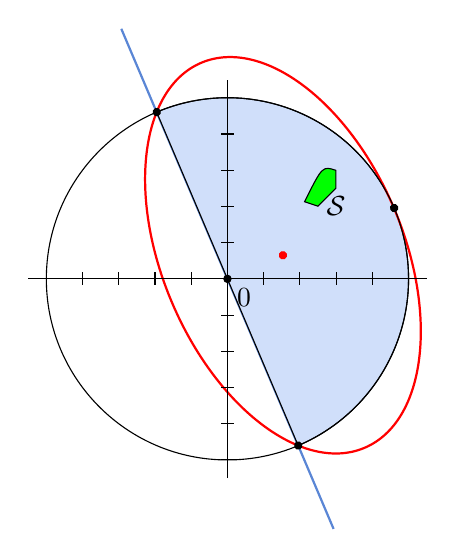
\begin{tikzpicture}[scale=2.3]

\begin{scope}[rotate=-157]
  \draw[draw=CornflowerBlue!90!black,thick] (0,-1.5) -- (0,1.5);
  \filldraw[ rotate=180, fill=CornflowerBlue!30, fill opacity=95] (0,-1) arc [start angle=-90, end angle=90, radius=1] -- cycle;
\draw[thick,draw=red] (-0.333,0) circle [x radius=0.666, y radius=1.1547];
\filldraw[red] (-0.333,0) circle [radius=0.02];

%\begin{scope}[shift={(-0.333,0)}]
%\draw[dashed, Salmon,  rotate=50] (0,-1.5) -- (0,1.5);
%\end{scope}

\filldraw (0,1) circle [radius=0.02];
\filldraw (0,-1) circle [radius=0.02] ;
\filldraw (-1,0) circle [radius=0.02] ;
\end{scope}
\filldraw[shift={(0.5,0.5)}, scale=0.07, rotate=45, draw=black, fill=green] 
      (-1,-1) -- (1,-1) -- (2,0) .. controls (1.5,1)  ..  (-1.5,0) -- cycle;
      \draw (0.6,0.4) node {$\cal S$};
\draw (0,0) circle [radius=1] node[anchor=north west] {$0$};
\filldraw (0,0) circle [radius=0.02];
%axis
\draw (-1.1,0) -- coordinate (x axis mid) (1.1,0);
\draw (0,-1.1) -- coordinate (y axis mid) (0,1.1);
%ticks
\foreach \x in {-1,-0.8,...,1}
\draw (\x,1pt) -- (\x,-1pt);
\foreach \y in {-1,-0.8,...,1}
\draw (1pt,\y) -- (-1pt,\y);

\end{tikzpicture}
\end{center}
\end{minipage}
\noindent  
  stred elipsy leží v $S$, 
  máme riešenie, inak 
  opäť existuje priamka prechádzajúca stredom elipsy tak, 
  že $S$ je v jednej polovici; môžeme nájsť najmenšiu
  elipsu opísanú príslušnej ''polelipse'' a takto pokračovať ďalej.
Pripomeňme, že elipsa $E$ so stredom v bode $(0,0)$ a jej plocha $\lVert E\rVert$ sú dané nasledovnými vzťahmi,
pričom $a$, $b$ sú dĺžky jednotlivých poloosí:

\begin{minipage}[t]{0.5\textwidth}
  \vskip 0pt
\begin{center}
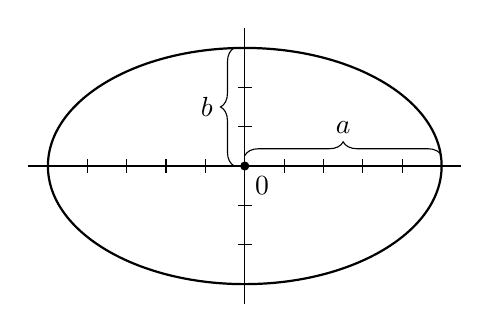
\begin{tikzpicture}[scale=2.5]

  \draw[thick] (0,0) ellipse (1.0 and 0.6)  node[anchor=north west] {$0$};
\filldraw (0,0) circle [radius=0.02];
%axis
\draw (-1.1,0) -- coordinate (x axis mid) (1.1,0);
\draw (0,-0.7) -- coordinate (y axis mid) (0,0.7);

 \draw [decorate,decoration={brace,amplitude=5pt,raise=5pt},xshift=0pt,yshift=-0.5pt] (0,0) -- (1,0)
  node[black,midway,yshift=15pt] {$a$};
 
  \draw [decorate,decoration={brace,amplitude=5pt,raise=5pt},xshift=0.5pt,yshift=0pt] (0,0) -- (0,0.6)
  node[black,midway,xshift=-15pt] {$b$};

%ticks
\foreach \x in {-1,-0.8,...,1}
\draw (\x,1pt) -- (\x,-1pt);
\foreach \y in {-0.6,-0.4,...,0.6}
\draw (1pt,\y) -- (-1pt,\y);


\end{tikzpicture}
\end{center}
\end{minipage}
\begin{minipage}[t]{0.5\textwidth}
  \vskip 0pt
  \begin{eqnarray*}
    E &=& \left\{ (x,y)\in\R^2\mid \frac{x^2}{a^2}+\frac{y^2}{b^2}\le1\right\} \\
    \lVert E\rVert & =& \pi a b
    \end{eqnarray*}
\end{minipage}


\noindent
Aby náš postup zafungoval, musíme vedieť nájsť najmenšiu elipsu opísanú generickej polelipse a ukázať, že jej plocha 
je o konštantný faktor menšia. Majme teda elipsu v ľubovoľnej polohe a priamku prechádzajúcu jej stredom. 
Začneme tým, že elipsu presunieme do bodu
$(0,0)$ a otočíme tak, aby jej osi boli rovnobbežné so súradnicovými osami. 


\begin{minipage}[t]{0.5\textwidth}
  \vskip 0pt
\begin{center}
\begin{tikzpicture}[scale=2.5]


\end{tikzpicture}
\end{center}
\end{minipage}
\begin{minipage}[t]{0.5\textwidth}
  \vskip 0pt
\begin{center}
\begin{tikzpicture}[scale=2.5]

\end{tikzpicture}
\end{center}
\end{minipage}


\IGNORE{
\vspace*{-4ex}
\noindent
\colorlet{shadecolor}{Aquamarine!9}
\begin{shaded}
\subsection*{Malá odbočka k elipsám}

\noindent
Čitateľ sa už možno stretol s konvexným obalom v dvoch rozmeroch: pre dané body
v rovine je ich konvexný obal najmenší konvexný mnohouholník, ktorý ich všetky obsahuje.

\end{shaded}



  elipsa opísaná polkruhu. Pozrime sa preto na elipsu trocha bližšie. Čitateľ si azda pamätá, že elipsa\footnote{% 
keď budeme hovoirť o elipse, vždy budeme myslieť elipsu aj s vnútrom} 
stredom v $[0,0]$ a poloosami $a$, $b$ je množina bodov $[x,y]$ v rovine, spĺňajúcich vzťah
$$\frac{x^2}{a^2}+\frac{y^2}{b^2}\le1$$
a jej plocha je $\pi ab$.

\begin{center}
\begin{tikzpicture}[scale=2.3]

% elipsa
\begin{scope} [rotate=-157]
\end{scope}


\end{tikzpicture}
\end{center}
}



% elipsoidova metoda
% bin packing (det. rounding)
%%, network design (iterative rounding), steiner tree (randomized rounding)
%% chernoff -multicomodity flow (random sampling)

% semidefinitne progr
% max cut

%%
%treba:  determinanty, matice, stredna hodnota, nahodne premenne, ag nerovnost, derivacie

%%%%%%%%%%%%%%%%%%%%%%%%%%%%%%%%%%%%%%%%%%%%%%%%%%%%%%%%%%%%%%%%%%%%%%

%\vfill
%\centerline{  * * * TO BE CONTINUED ... * * * }
%\vfill


\newpage
\bibliography{references}
\end{document}

